\documentclass[pregrado]{tesis-usb}

% paquetes
\usepackage[utf8]{inputenc}
\usepackage{verbatim}
\usepackage{acronym}
\usepackage{amsmath}
\usepackage{amsfonts}
\usepackage{amssymb}
\usepackage{enumitem}
\usepackage{multirow}
\usepackage{array}
\usepackage{float}
\usepackage{url}
\usepackage{xcolor}
\usepackage[belowskip=-5pt,aboveskip=10pt]{caption}
% \usepackage{hyperref}

% estilo de las referencias
\usepackage[fixlanguage]{babelbib-and}
\selectbiblanguage{spanish}
\usepackage{url}
\bibliographystyle{babunsrt-fl}

\autor{Esteban de Jesús Rafael Camargo Rodríguez}
\usbid{11-10145}
\titulo{Desarrollo de un simulador de adiestramiento para ingenieros y operadores de hornos de proceso}
\tutor{Prof. Antonio Cavero N.}
\usarcotutor
\cotutor{Prof. Euler Jiménez G.} 
\trabajo{Proyecto de grado}
\coord{Ingeniería Química}
\grado{Ingeniero Químico}
\fecha{Marzo~de~2023}

\autori{E. Camargo}
\agno{2023}
\fechadefensa{03~de~Marzo~de~2023}
\carrera{Ing. Química}

\programa{Nombre del Programa de Postgrado}
\juradouno{Alejandro Requena}
\juradodos{Sabrina D'Scipio \mbox{(Afiliación)}}
\juradotres{Claudio Olivares}

% Cambia comillas simple por comilla cerrada en ambiente verbatim 
\makeatletter
\let \@sverbatim \@verbatim
\def \@verbatim {\@sverbatim \verbatimplus}
{\catcode`'=13 \gdef \verbatimplus{\catcode`'=13 \chardef '=13 }} 
\makeatother

\begin{document}

\frontmatter
\maketitle
\chapter*{Dedicatoria}

\par Dedicado a la Universidad Sim\'on Bol\'ivar y a su comunidad.
\par A mis padres.

\chapter*{Agradecimientos}

Gracias a mis tutores, Euler y Antonio, por su gu\'ia en este trabajo, respondiendo atentamente a todas mis preguntas, por su paciencia corrigiendo mis errores y por su constante motivación.\\

Gracias a mi madre, Marlene, por apoyarme incondicionalmente y siempre haber creído en mí.
\begin{resumen}
    %\par La habilidad de operar hornos de proceso es fundamental en cualquier planta del sector petrolero, pero, el conocimiento práctico no es suficiente; no basta con saber modificar su condición de operación, también es necesario conocer los principios físicos que determinan el funcionamiento del equipo para lograr optimizar el proceso. 
    \par Se concibió este proyecto con el objetivo de desarrollar un simulador, que ayude a transmitir de manera efectiva los principios en la operación de un horno de proceso, simulando el comportamiento térmico del horno frente a las posibles variaciones de las condiciones operacionales; lo que permite que los usuarios puedan tener una referencia de cómo cambia el proceso dependiendo de las variables que se modifiquen.
    El horno usado es una unidad de tiro natural, tipo cabina, con serpentín radiante horizontal. Su diseño se realizó tomando como referencia el horno de una unidad de destilación a vacío existente en una refinería.
    Las variables modificables en la interfaz de entrada son: la cantidad de fluido de proceso que circula, las temperaturas de entrada o salida del fluido, el exceso de aire o el porcentaje de oxígeno en los gases de combustión, la humedad relativa y temperatura del aire ambiental, los factores de ensuciamiento, las pérdidas de calor del horno al ambiente y los componentes del gas combustible. Las principales variables calculadas son el consumo de combustible, la cantidad de CO$_2$ generado, la eficiencia térmica y las condiciones de temperatura en las diferentes zonas del horno.
    Se ofrecen tres opciones de resultados: 1) donde se puede comparar un resumen de los resultados de dos condiciones de operación; 2) donde se observan, en detalle, todos los resultados de una condición de operación; 3) donde se puede optar por graficar separadamente las tendencias de seis variables de salida con respecto a cuatro variables de entrada.\\
    \par El simulador está disponible en el enlace: \url{https://e-usb.github.io/heater}\\
     \vspace{10pt}\\
     Palabras clave: Horno de proceso, Fired heater, Combustión, Intercambiador, Simulador.
\end{resumen}
\tableofcontents
\listoffigures
\listoftables
\useacronyms
\chapter*{Lista de símbolos}
\begin{tabular}{ll}

$AC_{masa}$ & Relación aire/combustible másica [-] \\
$AC_{molar}$& Relación aire/combustible molar [-] \\
$Afo$   & Área de superficie externa de aletas [m$^2$] \\
$Apo$   & Área de superficie expuesta de tubos lisos [m$^2$] \\
$A_0$   & Área de superficie externa total [m$^2$] \\
$At$    & Área externa del banco de tubos por zona del horno [m$^2$] \\
$Acp$   & Área de plano equivalente por zona del horno [m$^2$] \\
\\
$C_{1,3,5}$ & Coeficientes del factor de Colburn \\
$C_p$   & Calor específico [kJ/kg-K] \\
$C_{p_a}$   & Calor específico del aire [kJ/kg-K] \\
$C_{p_c}$   & Calor específico del combustible [kJ/kg-K] \\
$C_{p_f}$   & Calor específico del fluido [kJ/kg-K] \\
$C_{p_g}$   & Calor específico de los gases de combustión [kJ/kg-K] \\

$d_f$ & Diámetro externo de la aleta [m] \\
$d_o$ & Diámetro externo del tubo [m] \\

$E$   & Eficiencia de las aletas [-]\\
$F$   & Factor global de transferencia radiante [-]\\
$G$   & Velocidad másica basada en el área interna de tubos radiantes [kg/h-m$^2$]\\
$G_n$ & Velocidad másica basada en el área libre para el flujo de gas [kg/h-m$^2$]\\
\\
$h_{c}$ & Coeficiente de transferencia de calor convectivo [W/m$^2$-K]\\
$h_{e}$ & Coeficiente de transferencia de calor externo [W/m$^2$-K]\\
$h_{ee}$& Coeficiente de transferencia de calor externo efectivo [W/m$^2$-K]\\
$h_{i}$ & Coeficiente de transferencia de calor interno [W/m$^2$-K]\\
$h_{r}$ & Coeficiente de transferencia de calor radiante [W/m$^2$-K]\\
\\
$j$     & Factor de Colburn [-] \\
$k_f$   & Conductividad térmica del fluido [W/m-K] \\
$k_g$   & Conductividad térmica de los gases de combustión [W/m-K] \\
\\
$\dot m_a$  & Flujo másico de aire [kg/h] \\
$\dot m_c$  & Flujo másico de combustible [kg/h] \\
$\dot m_f$  & Flujo másico de residuo de vacío [kg/h] \\
$\dot m_g$  & Flujo másico de los gases de combustión [kg/h] \\
\end{tabular}

\begin{tabular}{ll}
\\
\\
$n_a$  & Número de moles del aire [mol] \\
$n_c$  & Número de moles del combustible [mol] \\
\\
$l_f$   & Altura de aleta [m] \\
$L_{tubo}$ & Largo efectivo del tubo [m] \\
$N_r$   & Numero de tubos por fila [-] \\
$N_{tubo}$ & Número de tubos por sección [-] \\
\\
$PL$    & \multirow{2}{26em}{Multiplicación de las presiones parciales de CO$_2$ y H$_2$O por MBL [atm-ft]} \\
\\
$PM_a$    & Peso molecular del aire [kg/kmol]\\
$PM_c$    & Peso molecular del combustible [kg/kmol]\\
\\
$P_l$   & Paso de tubo longitudinal [-]\\
$P_t$   & Paso de tubo transversal [-]\\
\\
$Pr$    & Número de Prandtl [-]\\
\\
$Q_{a}$    & Calor sensible del aire [MW] \\
$Q_{absorbido}$ & Calor absorbido por el fluido en el horno [MW] \\
$Q_{c}$    & Calor sensible del combustible [MW] \\
$Q_{conv}$ & Calor transferido por convección [MW] \\
$Q_{CONV}$ & Calor cedido al fluido en la sección convectiva [MW] \\
$Q_{ESC}$ & Calor cedido al fluido en la sección escudo [MW] \\
$Q_{f_e}$ & Calor del fluido entrando [MW] \\
$Q_{f_s}$ & Calor del fluido saliendo [MW] \\
$Q_{g}$   & Calor sensible de los gases de combustión [MW] \\
$Q_{perdidas}$  & Pérdidas de calor al ambiente [MW] \\
$Q_{rad}$ & Calor transferido por radiación [MW] \\
$Q_{RAD}$ & Calor cedido al fluido en la sección radiante [MW] \\
$Q_{radEsc}$& Calor de radiación que pasa a la sección escudo [MW] \\
$Q_{suministrado}$ & Calor suministrado por combustión [MW] \\
\\
$q_{rad}$ & \multirow{2}{26em}{Flujo de calor por unidad de área exterior del tubo en zona radiante [MW/m$^2$]} \\
\\
$Re$    & Número de Reynolds [-]\\
\\
$R_{fi}$  & Factor de ensuciamiento interno de los tubos [m$^2$-K/W] \\
$R_{fe}$  & Factor de ensuciamiento externo de los tubos [m$^2$-K/W] \\
\end{tabular}

\begin{tabular}{ll}
\\
\\
$R_{int}$  & Resistencia convectiva interna [m$^2$-K/W]\\
$R_{ext}$  & Resistencia convectiva externa [m$^2$-K/W] \\
$R_{tube}$ & Resistencia conductiva del tubo [m$^2$-K/W]\\
$\Sigma R$ & Suma de las resistencias de transferencia de calor [m$^2$-K/W]\\
\\
$s_f$      & Espaciado de aleta [1/m]\\
$S_{tubo}$ & Espaciado de tubos [m] \\
\\
$T_b$ & Temperatura de mezcla del fluido por zona [K] \\
$T_{fe}$& Temperatura del fluido entrando al horno [K] \\
$T_{fs}$& Temperatura del fluido saliendo del horno [K] \\
$T_{fer}$& Temperatura del fluido entrando a la zona radiante [K] \\
$T_{fee}$& Temperatura del fluido entrando a la zona escudo [K] \\
$T_{gc}$& Temperatura de los gases de combustión a la salida de la zona convectiva [K] \\
$T_{ge}$& Temperatura de los gases de combustión a la salida de la zona escudo [K] \\
$T_{gr}$& Temperatura de los gases de combustión a la salida de la zona radiante [K] \\
$T_g$   & Temperatura efectiva de llama, equivalente a $T_{gr}$ [K] \\
$T_{gb}$& Temperatura de mezcla del gas por zona [K] \\
$T_s$ & Temperatura promedio de aleta [K]\\
\\
$U_0$ & Coeficiente de transferencia de calor global [W/m$^2$-K] \\
\\
$\sigma$    & Constante de Stefan-Boltzmann [W/m$^2$-K$^4$] \\
$\rho$      & Densidad [kg/m$^3$] \\
$\alpha$    & Factor de efectividad del banco de tubos [-]\\
$\gamma_r$  & Factor de radiación externo [-] \\
$\mu_f$     & Viscosidad del fluido [cP] \\
$\mu_g$     & Viscosidad de los gases de combustión [cP] \\
\end{tabular}

\setlength{\parskip}{6px}
\mainmatter
\chapter*{Introducción}

\par En refinerías de petróleo crudo, plantas químicas y petroquímicas, los hornos representan los equipos que suministran más del 80\% de la totalidad de la energía requerida para los procesos de separación y conversión química de los productos. Desde este punto de vista, la eficiencia energética de cada horno es una variable crítica a optimizar, con el fin de reducir el consumo de combustibles quemados, minimizar las emisiones de gases de combustión que, finalmente, se traducen en menores costos operativos [1].

\par Los \texttt{hornos de procesos} juegan un rol primordial en una refinería. Consumen altísimas cantidades de combustibles fósiles ({\tt miles de kilogramos por hora}) y emiten proporcionales cantidades de \ac{co2} a la atmósfera. Son equipos de alto costo que trabajan con llamas a muy altas temperaturas (\textgreater 2000 °C) y cuyas fallas suelen ser críticas para la economía de la refinería. Es importante destacar que el dióxido de carbono atmosférico promedio mundial en 2019 fue de 409,8 ppm, con un rango de incertidumbre de 0,1 ppm. Lo que indica que los niveles de dióxido de carbono resultaron los más altos de los últimos 800.000 años [2]. Teniendo como referencia las cifras del 2018 reportadas por la \ac{ONU}, 55,3 Gt\ac{co2}e (giga toneladas de \ac{co2} equivalente) [3], se puede apreciar el impacto significativo que esto genera sobre el medio ambiente. 

\par Lamentablemente, no es posible automatizar la totalidad de la operación de un horno de procesos [4] puesto que no son equipos completamente herméticos como un intercambiador de calor o una columna de destilación. Esta condición, es decir, estar "abiertos a la atmósfera", hace recaer sobre los operadores de sala de control y de campo (la interfase humano-horno), la responsabilidad última sobre el proceso de combustión y el aprovechamiento del combustible.  

\par Por experiencias prácticas, dentro de las refinerías se ha identificado que los operadores suelen manejar estos equipos con altos niveles de tiro y de exceso de aire, estas variables de operación están alejadas de las condiciones recomendadas al diseñar el horno, lo que conlleva mayores emisiones de CO2 al ambiente y además afecta la integridad mecánica del equipo. Los altos niveles de exceso de aire, provocados por altos niveles de tiro, traen consigo un mayor consumo del combustible para compensar el calor perdido al calentar el aire en exceso, lo que a su vez provoca alteraciones en las características de las llamas haciéndolas incidir directamente sobre los tubos de la sección radiante causando la coquización localizada de la carga dentro de los tubos. 

\par En virtud de la dependencia de los hornos de proceso de la intervención continua y acertada de sus operadores se hace perentorio fomentar su capacitación como una manera de incrementar el desempeño y la eficiencia de estos equipos. 

\par Por esta razón, se ha considerado necesario construir un simulador de hornos de procesos, con base en los estándares API 560 y API RP 535, para su utilización como herramienta práctica en la capacitación del personal operativo de las refinerías de petróleo. Esta herramienta permitiría, de una manera más didáctica, observar e interactuar con las variables fundamentales de control del horno, a saber, el tiro y el exceso de aire, para controlar los efectos de las operaciones alejadas de las condiciones de diseño.

\par Este proyecto utilizará ecuaciones de balance de masa y transferencia de calor para representar las condiciones de operación en un modelo gráfico capaz de responder a diferentes estímulos en las variables. 
\vfill
\par Esta es la versión \version~del documento de tesis para la \ac{USB}, creada y mantenida por:\\
\begin{tabular}{lc}
Br. Esteban Camargo & 11-10145@usb.ve 
\end{tabular}
\chapter{Antecedentes}

\par En este capítulo se desarrollan los puntos que respaldan este proyecto, como la justificación y objetivos. Adicionalmente se describen algunos proyectos que anteceden a la investigación y que se usaron como referencias.

\section{Justificación}

\par En virtud de que los hornos de proceso requieren de la intervención continua y acertada de sus operadores, se hace evidente la necesidad de fortalecer la capacitación de dichos operadores como una manera de incrementar la eficiencia en las condiciones de operación de estos equipos, lo que lograría disminuir la cantidad de emisiones que se arrojan al medio ambiente, disminuir el consumo de combustible, prolongar la vida útil del equipo y anticipar cambios en el proceso de una manera controlada.
\par Adicionalmente, para un estudiante o ingeniero que intente formarse en esta área los recursos para experimentar son limitados.
\par Por esta razón, se consideró necesario diseñar y desarrollar un simulador de hornos de proceso con base en los estándares API 560 \cite{bib:api560} y API RP 535 \cite{bib:api535}, para su utilización como herramienta práctica en la capacitación del personal operativo de las refinerías de petróleo, ya que las opciones de simuladores existentes no son abiertas al público y solo están enfocadas al diseño de hornos.
\par Esta herramienta debe permitir, de una manera didáctica, observar e interactuar con las variables fundamentales de control del horno, a saber: el exceso de aire en la combustión, la composición del combustible, la carga de flujo a manejar y las temperaturas de entrada y salida del fluido al horno; con el fin de simular y comparar los efectos de operar el horno alejado de las condiciones óptimas de diseño.

\section{Objetivos}

\subsection{Objetivo General}

\par Desarrollar un simulador web de hornos de proceso de tiro natural que pueda ser fácilmente utilizado para la enseñanza del manejo de estos equipos, al permitir visualizar los efectos de modificar los valores de las variables que gobiernan el proceso y su importancia en la eficiencia del equipo.

\subsection{Objetivos específicos}

\par Aplicar los diferentes conceptos asociados a la operación de hornos de proceso.

\par Aplicar las ecuaciones de balance de masa y energía, y las ecuaciones de transferencia de calor en la construcción del modelo matemático para el cálculo de las condiciones de operación de los hornos de proceso.

\par Diseñar una herramienta para la enseñanza de la operación de los hornos de proceso, usando un algoritmo basado en el modelo matemático anterior, con una interfaz de entrada y salida de datos amigable para los usuarios, con la que se simulen las modificaciones de las condiciones de proceso de un horno.

\par Desarrollar la herramienta mencionada e integrarla a una interfaz en línea, tomando ventaja del desarrollo de tecnologías web libres, que permita el acceso desde cualquier dispositivo con internet y aumente el alcance de dicha herramienta.

\section{Proyectos Previos}

\par Existen investigaciones enfocadas en la optimización de hornos de proceso particulares con características y condiciones definidas \cite{bib:leti}; también existen distintos simuladores enfocados en el diseño de hornos, pero no se ha encontrado un estudio con un alcance mayor, que intente analizar todo el comportamiento del horno en condiciones distintas a las de diseño, que también son observadas en la práctica y responden a un carácter académico.

\par También existen simuladores comerciales con enfoques orientados al diseño, pero ninguno con fines explícitamente educativos.

\par Lo innovador de este proyecto consiste en hacer como objetivo del simulador un aporte educacional y no una herramienta de diseño, con muchas aplicaciones que, además, pueden ampliarse si se continua desarrollando la interfaz con el algoritmo de base.
\chapter{Marco Teórico}

\par En este capitulo se trataran las bases teóricas necesarias para desarrollar los modelos matemáticos y realizar los cálculos que se usaran luego en la sección metodológica. 

Ecuaciones
Descripción de los fenómenos
Conceptos
Variables

\section{Secciones}

\par El horno puede ser dividido en secciones para simplificar los cálculos, las cuatro secciones b\'asicas son las siguientes:

\subsection{Combustión}
\subsection{Radiación}
\subsection{Escudo}
\subsection{Convección}
\chapter{Marco Metodológico}

\par En este capitulo se describirá la secuencia del algoritmo desarrollado para el cálculo de las variables por sección en el horno. 

En primera instancia se hará una reseña histórica de las ecuaciones cubicas del tipo van der Waals. 
Se continuara con una corta revisión de la ecuación virial y sus implicaciones para la traslación volumétrica dependiente de la temperatura. 
Posteriormente se detallaran a fondo las bases de las traslaciones volumétricas, desde su origen hasta su estatus hoy en día. Finalmente, se tocara el tema del principio delos estados correspondientes, y su extensión a tres y cuatro parámetros, dentro de los cuales se enmarcaría la traslación volumétrica.

\section{Inicialización}

\par Usar la clase se hace de la mi
\chapter{Interfaz del simulador y alojamiento web}
\par En este capítulo se describe la interfaz gráfica diseñada para interactuar con el simulador, consistente en pantallas de introducción de datos y pantallas para mostrar los resultados del simulador. Adicionalmente, se describe la plataforma usada para alojar el simulador en la web.

\section{Interfaz de usuario (UI)}
\par Una interfaz de usuario (UI, abreviación comúnmente usada en inglés) es el medio por el cual una persona interactúa con una aplicación de software o dispositivo de hardware. Esto significa que el programa incluye controles gráficos que optimizan la experiencia de usuario usando un ratón, teclado o pantalla táctil.
\par Los elementos más comunes de una interfaz gráfica de usuario, de acuerdo con Career Foundry \cite{ui}, son:
\begin{itemize}
\item Controles de entrada: permiten introducir información en el sistema por parte de los usuarios.
\item Componentes de navegación: ayudan a los usuarios a moverse.
\item Componentes informativos: brindan información a los usuarios.
\item Contenedores: mantienen el contenido organizado, como paneles, ventanas, marcos, etc.
\end{itemize}
\par Sin la interfaz de usuario, el algoritmo, aunque poderoso, tendría un uso muy limitado por la complejidad que implica correrlo directamente como un programa y por lo difícil que es observar los cambios sin una amigable visualización de datos.
\par La interfaz de usuario implementada para el algoritmo se desarrolló usando los lenguajes básicos de desarrollo web: Lenguaje de Marcado de Hipertexto (HTML), Hojas de Estilo en Cascada (CSS) y el lenguaje de programación interpretado JavaScript (JS), lo que hace que sea totalmente editable y pueda correr en cualquier ordenador o dispositivo móvil con navegador web sin instalar otro programa. 
\par La interfaz desarrollada consiste en un sitio web donde el usuario puede navegar a distintas vistas con diferentes propósitos. A continuación se describirán dichas vistas y sus aplicaciones pensadas, esencialmente las posibilidades educativas que ofrece la comparación de dos estados del proceso, pero no limitadas a estas.

\subsection{Descripción de uso y alcances}
\par Al ingresar al enlace del simulador, la vista de bienvenida otorga instrucciones y limitaciones de uso del simulador, al ser la vista principal el usuario podrá conocer todas las capacidades y aplicaciones disponibles en la versión actual publicada (ver la Figura \ref{fig:alcance}).
\par Aquí se describen las condiciones de operación de diseño establecidas para dar una referencia al usuario de las cargas que puede manejar el horno simulado dentro de los rangos sugeridos de uso.
\begin{figure}[H]
\begin{center}
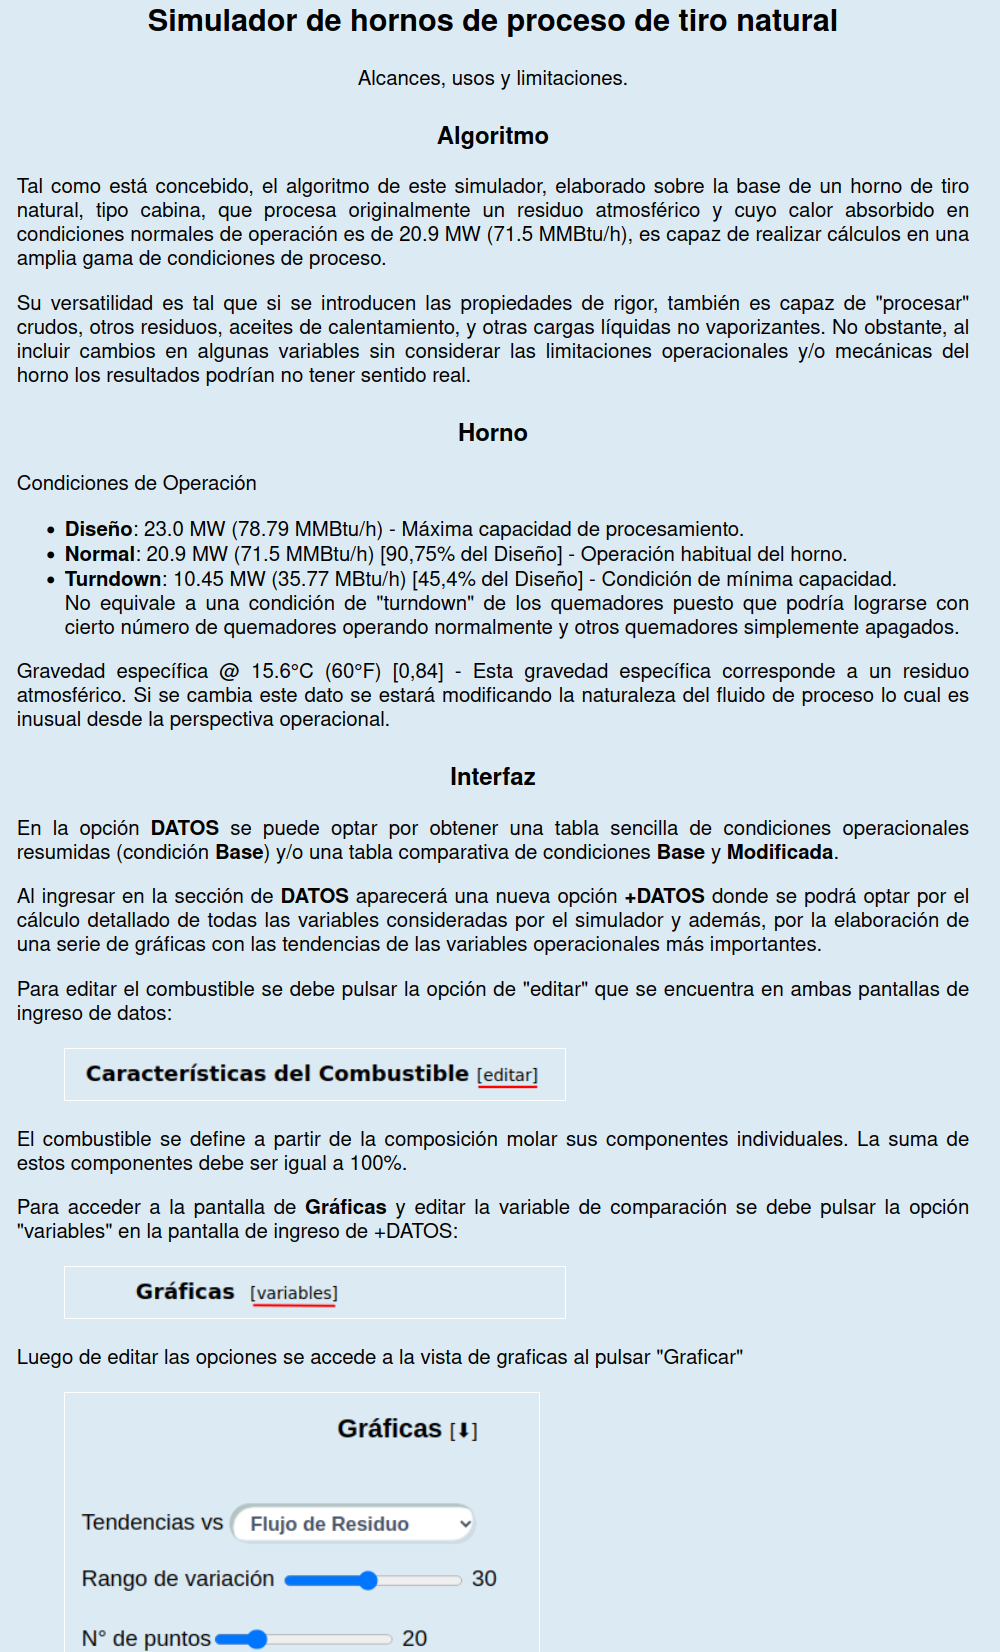
\includegraphics[scale=0.33]{images/alcance}
\caption[Página de alcances]{Referencia a página de alcances, vista introductoria a la aplicación web.}
\label{fig:alcance}
\end{center}
\end{figure}
\par La sección de usos y alcance describe como utilizar la barra de navegación del sitio web (ver Figura \ref{fig:navbar}), como editar el combustible a utilizar en las diferentes vistas de ingreso de datos y finalmente como usar la sección de gráficas o tendencias.
\begin{figure}[H]
\begin{center}

\includegraphics[scale=0.22]{images/navbar}
\caption[Barra de navegación]{Barra de navegación de la interfaz web.}
\label{fig:navbar}
\end{center}
\end{figure}

\subsubsection{Condiciones de operación de diseño mostradas}
\par En esta vista se detallan las condiciones de diseño, como se muestra a continuación:
\begin{itemize}
    \item \textbf{Diseño}: 23,0 MW (78,79 MMBtu/h) - Máxima capacidad de procesamiento recomendada.
    \item \textbf{Normal}: 20,9 MW (71,5 MMBtu/h) [90,75\% del Diseño] - Operación habitual del horno.
    \item \textbf{Turndown}*: 10,45 MW (35,77 MBtu/h) [45,4\% del Diseño] - Condición mínima de operación.
\end{itemize}
\par *No equivale a una condición de ``turndown'' de los quemadores puesto que podría lograrse con cierto número de quemadores operando normalmente y otros quemadores simplemente apagados.

\subsection{Introducción de datos}
\par En esta sección se desarrollan dos vistas:
\begin{itemize}
    \item La primera, que se accede al pulsar el botón \textbf{DATOS} en la barra de navegación, es una vista simplificada para introducir solo los datos más relevantes del proceso. Al accionar el cálculo dirige al usuario a una pantalla de resultados donde se pueden comparar dos estados de operación (ver Fig. \ref{fig:datos}).
\end{itemize}
\begin{figure}[H] \begin{center}
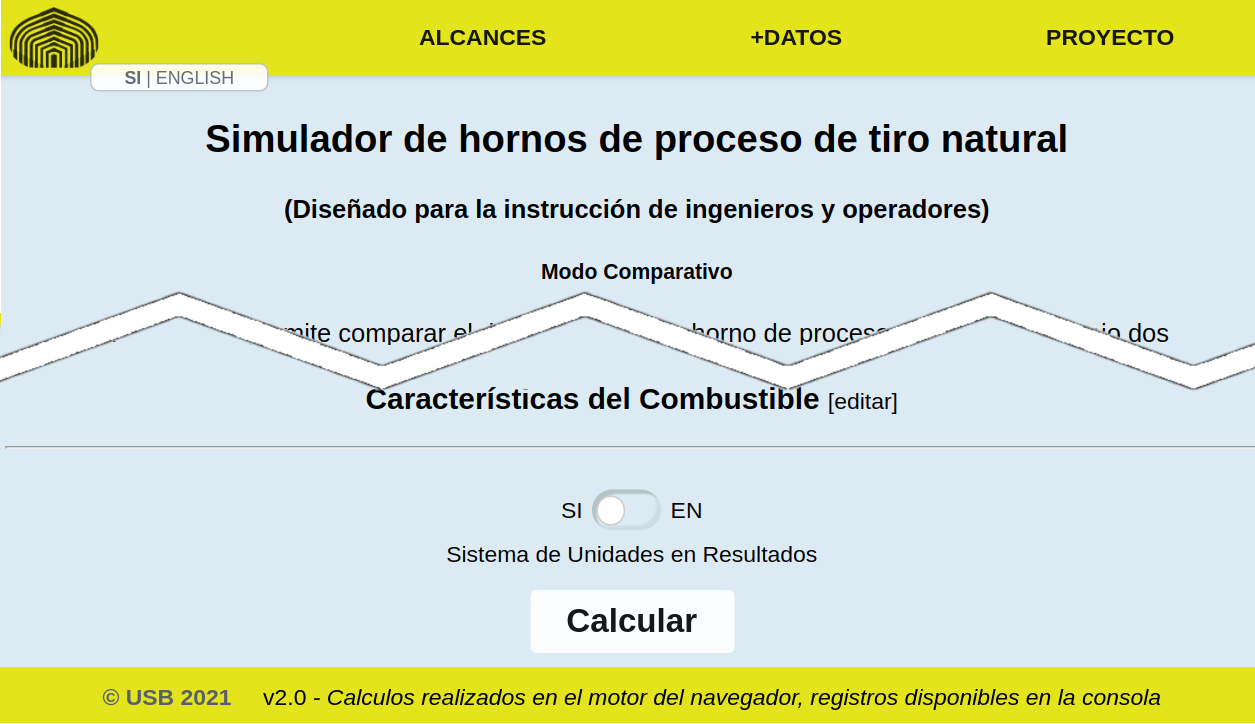
\includegraphics[scale=0.3]{images/datos}
\caption[Página de ingreso de datos para comparación]{Referencia a página de ingreso de datos utilizada para accionar el cálculo en la vista comparativa de resultados.}
\label{fig:datos} \end{center} \end{figure}
\begin{itemize}
    \item La segunda, que se accede estando en la sección de ingreso de datos simplificada al pulsar el botón \textbf{+DATOS} en la barra de navegación. En esta vista se encuentran todas las variables que permite modificar el proceso (ver Fig. \ref{fig:fulldatos}) y permite la posibilidad de accionar el cálculo para ofrecer una página de resultados extendidos. Adicionalmente se pueden accionar la generación de las curvas de tendencia escogiendo una variable a ser modificada al final de la página y pulsando el botón de graficar.
\end{itemize}
\begin{figure}[H] \begin{center}
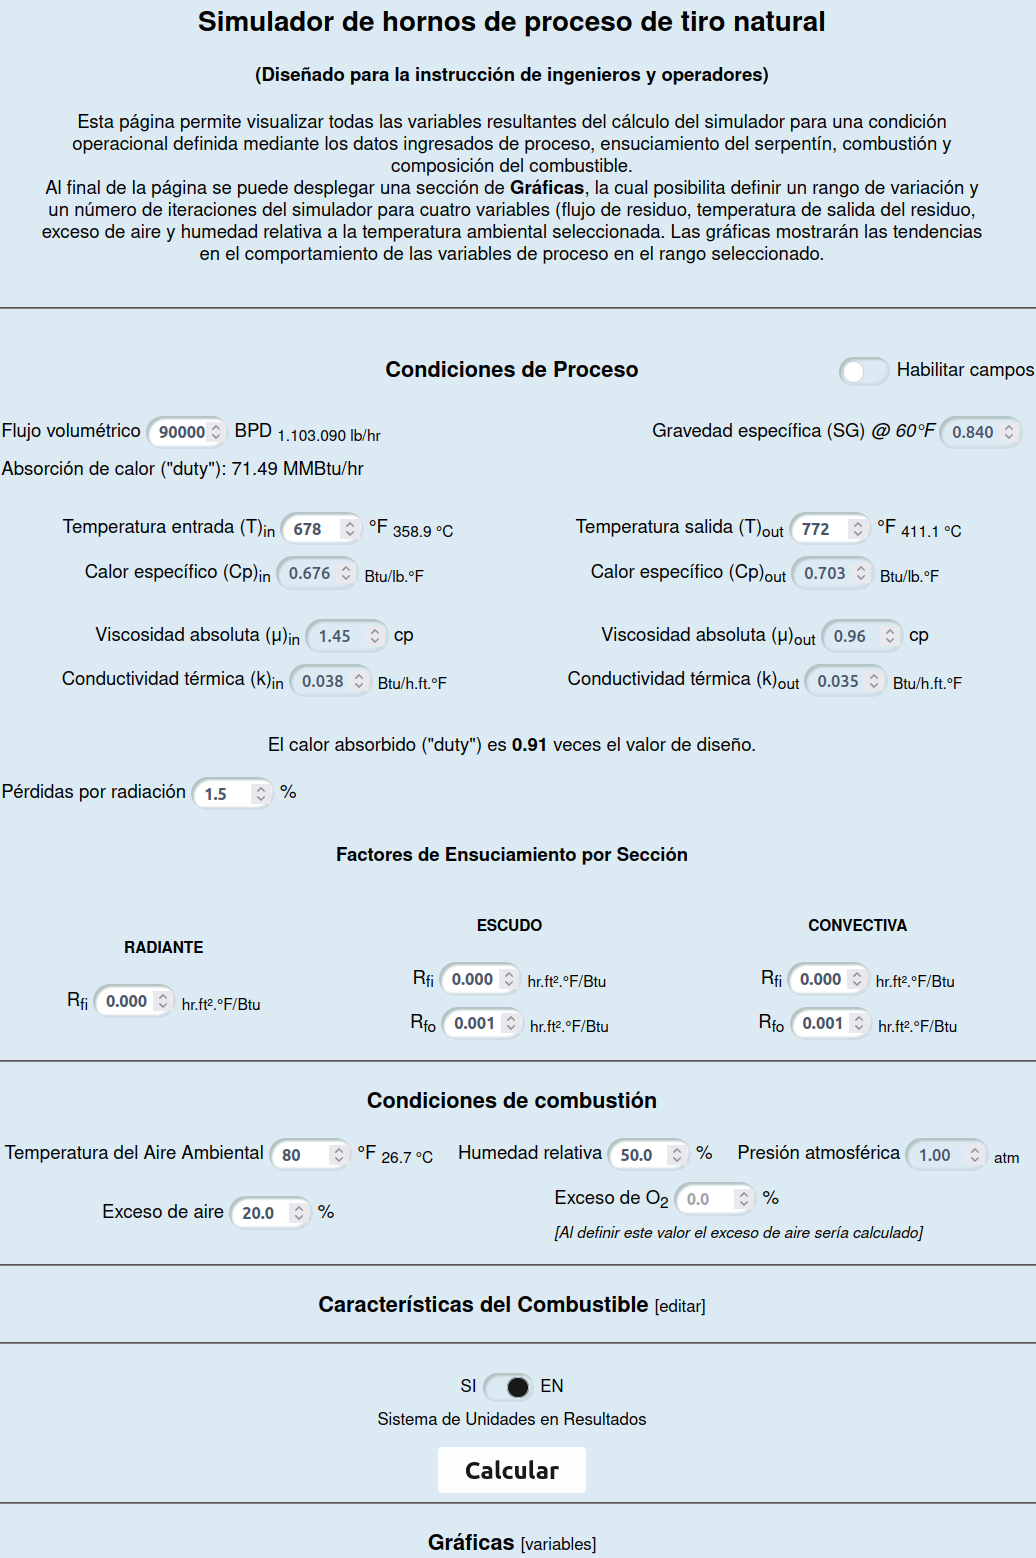
\includegraphics[scale=0.3]{images/datos2}
\caption[Página de ingreso de datos extendida]{Referencia a página de ingreso de datos extendida, con la opción de accionar la vista de resultados extendidos o la generación de gráficas de tendencia.}
\label{fig:fulldatos}
\end{center} \end{figure}
\par En ambas se puede modificar la composición molar del combustible al pulsar la opción ``editar'', como se muestra en la Figura \ref{fig:edit_fuel}:
\begin{figure}[H] \begin{center} 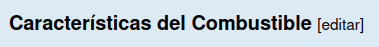
\includegraphics[scale=0.6]{images/edit_fuel}
\caption[Opción para editar el combustible]{Opción para editar el combustible al ingresar los datos.}
\label{fig:edit_fuel} \end{center} \end{figure}
\par Un ejemplo de los campos abiertos para la edición de la composición del combustible se puede apreciar en la Figura \ref{fig:edit_fuel_ext}:
\begin{figure}[hbt] \begin{center}
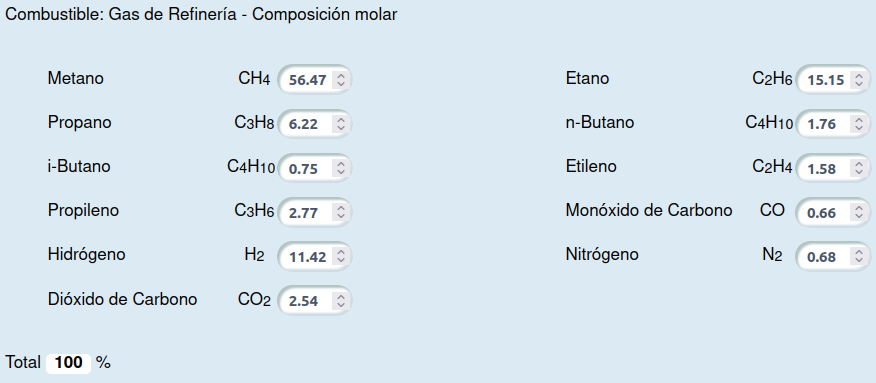
\includegraphics[scale=0.45]{images/edit_fuel_ext}
\caption[Campos para editar la composición del combustible]{Campos para editar la composición del combustible.}
\label{fig:edit_fuel_ext} \end{center} \end{figure}

\subsection{Resultados comparativos}
\par Esta vista es el resultado de accionar el cálculo en la sección de ingreso de datos simplificada. Posee el mayor potencial educativo, al resumir todas las variables resultantes y hacer una comparación entre dos condiciones de operación (Fig. \ref{fig:resultados}).
\par Aquí se pueden observar directamente los cambios en variables de interés, como los datos de ingreso, las emisiones de dióxido de carbono, el consumo de combustible, la distribución de calor dentro del horno, la temperatura de salida de los gases de combustión y la eficiencia térmica.
\par La recomendación para su uso es modificar solo una variable a la vez para su correcta interpretación.
\begin{figure}[H] \begin{center}
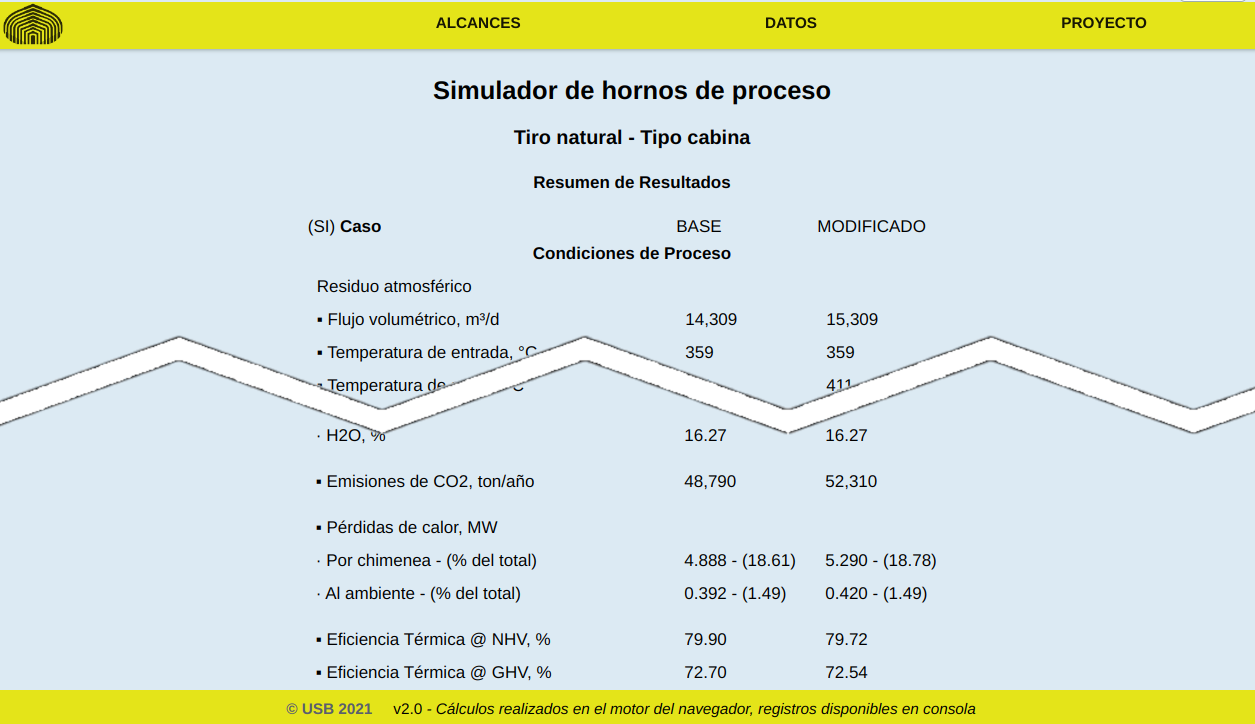
\includegraphics[scale=0.3]{images/result}
\caption[Página comparativa de resultados]
{Referencia a página comparativa de resultados, donde se pueden detallar los cambios de un estado a otro en la operación del horno.}
\label{fig:resultados} \end{center} \end{figure}

\subsection{Resultados extendidos}
\par Esta vista es el resultado de accionar el cálculo en la sección de ingreso de datos extendidos. Aquí se detallan todas las variables resultantes por cada sección del horno (Fig. \ref{fig:fullresultados}), se puede escoger el sistema de unidades a expresarse en la pantalla anterior, se uso extensamente al depurar las ecuaciones internas del algoritmo para encontrar sus puntos críticos y corregirlos.
\begin{figure}[H] \begin{center}
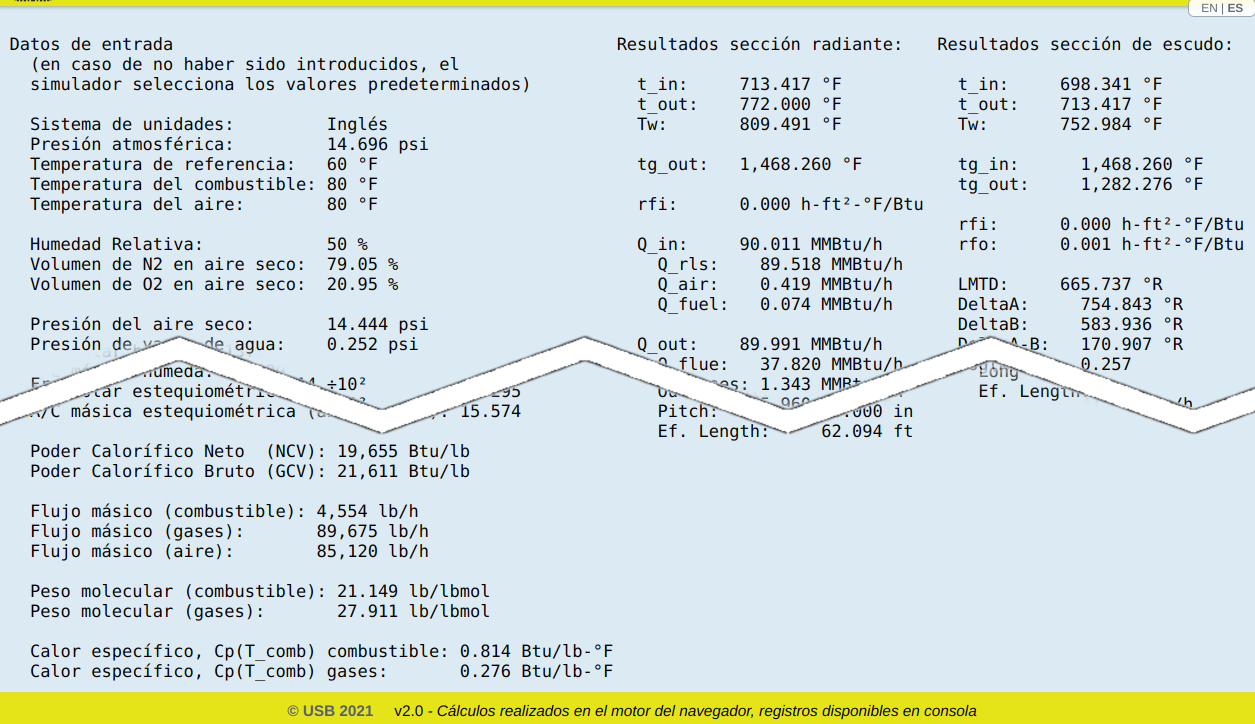
\includegraphics[scale=0.3]{images/result2}
\caption[Página extendida de resultados]{Referencia a página extendida de resultados, en ella se pueden observar a detalle las variables internas del proceso simulado.}
\label{fig:fullresultados} \end{center} \end{figure}
\par El objetivo de esta vista es tener una visión del comportamiento de todas las variables en el proceso, de aquí se pueden encontrar explicaciones no tan obvias del comportamiento de las variables finales mostradas en la vista comparativa.

\subsection{Gráficas}
\par Esta página es pensada para los usuarios más curiosos, y para futuras modificaciones del algoritmo o extensión de sus rangos (ver Figura \ref{fig:graficas}).
\begin{figure}[H]\begin{center}
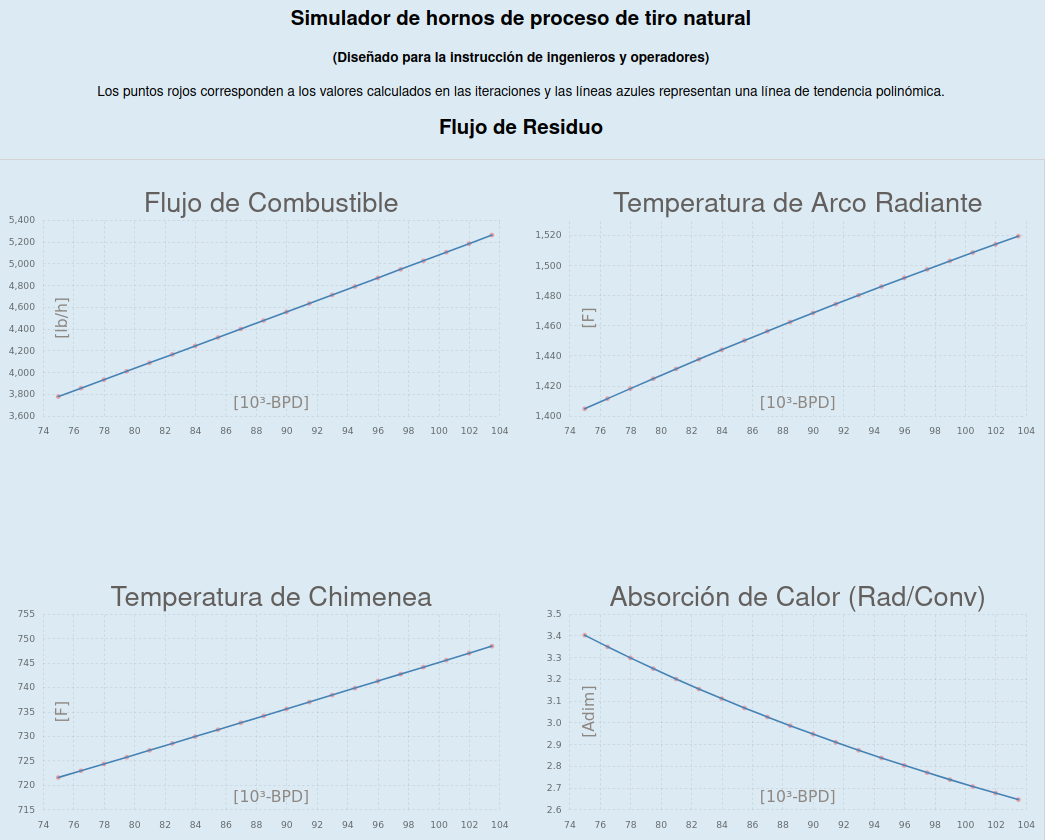
\includegraphics[scale=0.36]{images/graficas.png}
\caption[Página de gráficas]{Referencia de la página de gráficas, aquí se muestran las tendencias de las variables resultantes escogidas en el rango de variación determinado por el usuario.}
\label{fig:graficas} \end{center} \end{figure}
\par Para acceder a esta vista se debe accionar la opción de graficar ubicada al final de la página de ingreso de datos extendidos.
\par Su propósito es generar una visual del comportamiento del horno simulado a lo largo de un rango seleccionado, se usó para conseguir zonas donde los métodos aproximados del simulador no convergían y permitió sintonizar el paso, numero de iteraciones, valor inicial y tolerancia de dichos métodos.
\par En esta vista se pueden comprobar las tendencias, la continuidad y la estabilidad de las variables resultantes; también facilita la comprensión de los resultados de los fenómenos dentro del horno.

\section{Despliegue del simulador en la web}
\par En el apartado ``PROYECTO'' de la barra de navegación en la interfaz, mostrado en la Figura \ref{fig:navbar}, se puede acceder al repositorio del proyecto, ubicado en GitHub, servidor que aloja el software del simulador y lo mantiene en línea.
\par GitHub es una plataforma de alojamiento de código para el control de versiones y la colaboración. Permite trabajar de forma individual o en equipos para desarrollar proyectos con acceso desde cualquier lugar con conexión a internet.
\par Adicionalmente permite publicar sitios web estáticos, que no requieran manejo de base de datos en la nube o procesamiento de datos a nivel del servidor, para proyectos de código abierto.
\par Se usó esta ventajosa función para hacer el simulador accesible desde cualquier navegador y se encuentra disponible en el siguiente enlace: \url{https://e-usb.github.io/heater}
\par Para acceder al código alojado en GitHub se puede seguir el mismo enlace ubicado en la pestaña ``PROYECTO'' de la interfaz del simulador. \url{https://github.com/e-usb/heater}
\chapter{Especificaciones del horno simulado}

\par En este capítulo se describen las especificaciones del horno a simular, condiciones de operación de diseño y características mecánicas; también se detalla la composición del combustible y características del aire ambiental utilizado para la combustión.

\section{Descripción del horno a simular}
\par El horno seleccionado para simular en este proyecto fue uno de tipo cabina con serpentín horizontal de tiro natural, de fuego directo simple y de dos pasos para el fluido, descrito en la Figura \ref{fig:diagrama-vista}.
\par Esta basado en el horno de una unidad de destilación al vacío de una refinería en operación. El residuo de vacío, por tratarse de un fluido proveniente de la unidad de destilación atmosférica puede considerarse que la vaporización dentro del serpentín de tubos es muy baja y no se toma en cuenta en los cálculos.
\par Utilizando las condiciones de operación de una hoja de datos del horno de residuo de vacío, se estableció la condición de operación del horno simulado como se muestra en la Tabla \ref{tbl:capacidad}.
\begin{table}[H]\begin{center}
\caption[Condición de operación de diseño del horno]{Condición de operación de diseño del horno simulado}
\label{tbl:capacidad}\begin{tabular}{c|c|c|c|c}
Capacidad de carga& $\Delta$T& Flujo Vol.   & Grav. Esp.& Flujo Másico\\
23 MW 	          & 52 °C    & 15,723.0 m3/d& 0.84      & 15,723.0 toneladas/d
\end{tabular}\end{center}\end{table}
\begin{figure}[H]
\begin{center}
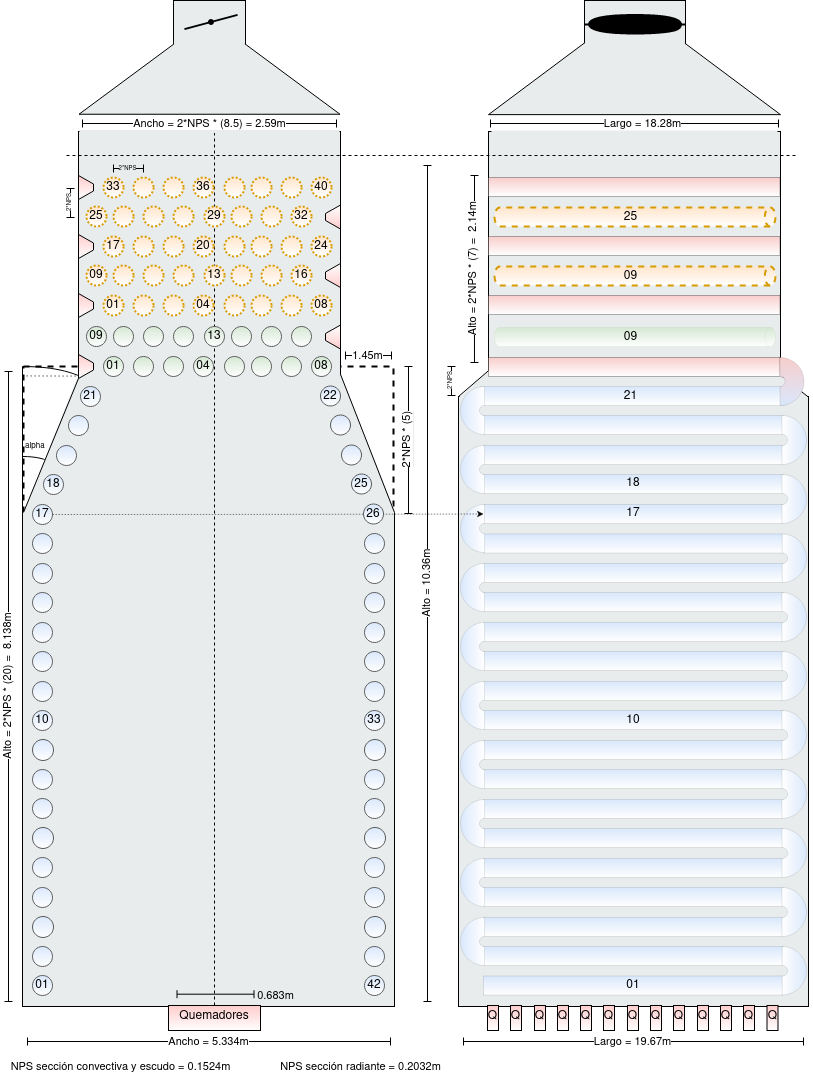
\includegraphics[scale=0.4]{images/diagrama-vista}
\caption[Cortes transversales del horno]{Cortes transversales del horno simulado.}
\label{fig:diagrama-vista}
\end{center}
\end{figure}

\subsection{Características mecánicas del horno seleccionado}
\par Lo primero a considerar en el diseño mecánico del horno fueron los tubos, se colocaron suficientes tubos para permitir la transferencia de calor equivalente a 70\% del calor requerido por el fluido de proceso en la sección de radiación.
\par El horno es de dos pasos, lo que significa que el fluido se divide en dos tuberías antes de ingresar, considerando la caída de presión para el diámetro nominal de los tubos. En la cámara de combustión, observada en la Figura \ref{fig:firebox}, se definió el ancho para cumplir con la relación alto/ancho establecida en el estándar API 560 \cite{bib:api560} y el resto de las medidas provienen de la separación y distribución de los tubos por sección sugeridas por el estándar.
\par En la Tabla \ref{tbl:firebox} se muestran las dimensiones resultantes de la cámara de combustión, son mostradas en pies y metros para su correspondiente uso en el cálculo de \ac{mbl}, resultando en la Ecuación \ref{eq:mbl} para el horno simulado.
\par Se puede observar a detalle cada una de las dimensiones de la configuración del horno en la Figura \ref{apx:img} ampliada en los anexos.
\begin{figure}[hbt] \begin{center}
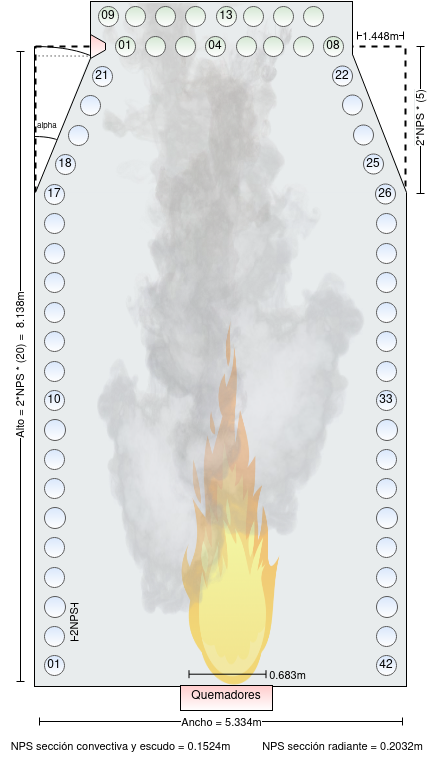
\includegraphics[scale=0.455]{images/firebox}
\caption[Diagrama de la cámara de combustión]{Diagrama de la cámara de combustión (sección radiante) del horno simulado.}
\label{fig:firebox} \end{center} \end{figure}
\begin{table}[H] \begin{center}
\caption[Dimensiones de la cámara de combustión]{Dimensiones de la cámara de combustión, mostrada en pies para su uso en la ecuación \ref{eq:pl} y la Tabla \ref{tbl:mbl}}
\label{tbl:firebox} \begin{tabular}{c|c|c}
Altura interna	&  8.354 m & 27.407 ft\\
Largo interno 	& 19.675 m & 64.552 ft\\
Ancho interno 	&  5.334 m & 17.500 ft\\
\end{tabular} \end{center} \end{table}
\begin{equation} \label{eq:mbl}
    MBL = 2/3 * (Alto*Largo*Ancho)^{1/3} = 20.829ft = 6.349m
\end{equation}
\par La descripción detallada de las característica de los tubos y aletas usadas se puede encontrar en la Tabla \ref{tbl:tubes} y una vista en perspectiva de la distribución de los tubos se puede apreciar en la Figura \ref{fig:diagrama-vista} al inicio de este capítulo.
\begin{table}[hbt]
\begin{center}
\caption[Distribución de tubos en el horno]{Distribución de tubos en el horno}
\label{tbl:tubes}
\begin{tabular}{l|c|c|c}
Sección 					& Radiante	& Escudo		& Convectiva \\
\hline
Material de tubos			& \multicolumn{3}{c}{-- A-312 TP321 --} \\

Soporte de tubos    		& Interno	& Externo		& Externo		\\
Arreglo	de tubos    		& Paralelo	& Escalonado	& Escalonado	\\
No. de pasos del fluido		& 2	        & 2	            & 2	            \\
No. de tubos total    		& 42		& 16			& 40			\\
No. de tubos por fila		& 2			& 8				& 8				\\
Grosor pared de tubos, cm	& 0.818		& 0.711			& 0.711			\\
Di. interno de tubos, cm	& 7.981		& 16.827		& 16.827		\\
Espaciado de tubos, cm  	& 40.640	& 				& 				\\
Espaciado transversal, cm  	&			& 30.480		& 30.480		\\
Espaciado longitudinal, cm 	&			& 30.480		& 30.480		\\
Largo de tubos efectivo, m	& 18.926    & 18.288		& 18.288		\\
\hline
Material de aletas			&			& 				& 11.5-13.5Cr	\\
Tipo de aletas				&			& 				& Solidas		\\	
Altura de aletas, cm		&			& 				& 2.438			\\
Grosor de aletas, cm		&			& 				& 0.152			\\
Densidad de aletas, aleta/m	&			& 				& 196.850		\\
\end{tabular} \end{center} \end{table}
\par La conductividad térmica de los tubos se calcula a traves de la ecuación:
\begin{equation}
k_w = (14.643 + 1.64e-2*T - 2e-6*T^2)*3.6 \quad [kJ/h.m^{\circ} C)]
\end{equation}
\par Se estableció que estas variables de diseño mecánico del horno no pueden ser modificadas por el usuario del simulador, a menos que se edite directamente el código.

\subsection{Condiciones de diseño para el combustible y el aire}
\par Como combustible se utilizó un gas de refinería por tratarse de un subproducto de las operaciones de refinación. La composición molar establecida por defecto, y usada para hacer la comprobación del algoritmo en el siguiente capítulo, se describe en la Tabla \ref{tbl:combustible}. Sin embargo, la posibilidad de cambiar la composición está abierta en la interfaz del simulador.
\par El aire ambiental establecido contiene humedad, definida a través de la humedad relativa y la temperatura; el cual en base seca solo considera nitrógeno y oxígeno, otros compuestos, como el argón, dióxido de carbono y otras trazas, son tomados dentro del contenido de nitrógeno por sus aportes del 1\% o menos a las ecuaciones de combustión.
\begin{table}[hbt]\begin{center}
\caption[Composición molar del gas de refinería]{Composición molar del gas de refinería para comprobación.}
\label{tbl:combustible}\begin{tabular}{l|r}
	Gas combustible					& (Moles \%) \\
	\hline
	Metano ($CH_4$)					& 56.47 \\
	Etano ($C_2H_6$)				& 15.15 \\
	Propano ($C_3H_8$)				& 6.22 \\
	n-Butano ($C_4H_{10}$)			& 1.76 \\
	i-Butano ($C_4H_{10}$)			& 0.75 \\
	Etileno ($C_2H_4$)				& 1.58 \\
	Propileno ($C_3H_6$)			& 2.77 \\
	Monóxido de carbono ($CO$)		& 0.66 \\
	Dióxido de carbono ($CO_2$)		& 2.54 \\
	Hidrógeno ($H_2$)				& 11.42 \\
	Nitrógeno ($N_2$)				& 0.68 \\
	Agua ($H_2O$)					& 0.00 \\
	Oxigeno ($O_2$)					& 0.00 \\
	Sulfuro de hidrógeno ($H_2S$)	& 0.00 \\
\end{tabular}\end{center}\end{table}
\par Como se describió en la sección de combustión del capítulo 2, la composición tomada para el aire seco es 20.95\% de oxígeno y 79.05\% de nitrógeno.
\begin{table}[hbt]\begin{center}
\caption[Características del aire]{Características del aire usado en la comprobación.}
\label{tbl:aire}\begin{tabular}{l|r}
	Exceso de aire, \%								& 20.000 \\
	Humedad relativa, \%							& 50.000 \\
	Temperatura del aire, °C						& 26.667 \\
\end{tabular}\end{center}\end{table}
\chapter{Resultados}

\section{Reacciones de combustión y requerimiento de aire}
\par Al ejecutar el cálculo de combustión con los datos de composición de combustible y condiciones ambientales de las las Tablas \ref{tbl:combustible} y \ref{tbl:aire}, se obtuvieron los resultados mostrados en la Tabla \ref{tbl:combustion-data}. Adicionalmente, se generaron las composiciones molar y másica de los gases de combustión mostradas en la Tabla \ref{tbl:combustion-gas}.
\begin{table}[hbt] \begin{center}
\caption[Combustión simulada]{Combustión simulada.}
\label{tbl:combustion-data} \begin{tabular}{l|c}
	A/C másica teórica requerido					& 15,574 \\
	A/C másica húmeda con exceso de aire			& 18,689 \\
	Relación de gases de combustión por unidad de aire& 19,689 \\
	Poder Calorífico Neto  (NCV), kJ/kg				& 45.718,6 \\
	Poder Calorífico Bruto (GCV), kJ/kg				& 50.268,0 \\
	Peso Molecular (PM) del combustible, kg/kmol	& 21,149 \\
	PM de los gases de combustión, kg/kmol				& 27,911 \\
\end{tabular} \end{center} \end{table}
\begin{table}[htb] \begin{center}
\caption[Composición de los gases de combustión]
{Composición porcentual de los gases de combustión.}
\label{tbl:combustion-gas} \begin{tabular}{l|c|c|c}
	   & \% Peso & \% Moles \\
	\hline
	Nitrógeno ($N_2$)			& 72,121	& 71,860 \\
	Oxígeno ($O_2$)				& 3,636 	& 3,172	 \\
	Dióxido de carbono ($CO_2$)	& 13,753	& 8,723	 \\
	Vapor de agua ($H_2O$)		& 10,490	& 16,245 \\
	Dióxido de azufre ($SO_2$)	& 0,000 	& 0,000	 \\
\end{tabular} \end{center} \end{table}

\par Para validar la confiabilidad de estos resultados del simulador se compararon con los obtenidos empleando el software comercial WinHeat\copyright\ para el diseño y evaluación de hornos, propiedad de Esteem Projects Pvt. Ltd., con una licencia autorizada para la versión 3.0. La conclusión de esta comparación arrojó que la diferencia entre los resultados de ambos simuladores para el cálculo de la combustión es menor a 0,1\%. 
\section{Simulación térmica del horno}
\par Los datos específicos del fluido y condiciones de operación que quedan por definir se muestran en la siguiente Tabla \ref{tbl:props}:
\begin{table}[htb]\begin{center}
\caption[Datos del fluido y condiciones de operación]{Datos del fluido y condiciones de operación}
\label{tbl:props}\begin{tabular}{l|c|c}
	Flujo del residuo atmosférico a calentar  & \multicolumn{2}{c}{12.019,6 toneladas/día} \\
	\hline
    Propiedades del residuo  & Entrada   & Salida \\
    Temperatura          (°C)       & 359    & 411 \\
	Viscosidad	         (cp)	    & 1,45	& 0,96 \\
	Capacidad calorífica (kJ/kg°C)	& 2,83 	& 2,943	 \\
	Conductividad térmica (kJ/h m²°C) & 0,230& 0,235	 \\
	\hline
	Factores de ensuciamiento & Interno & Externo\\
	Sección radiante	(m²°C/W)  & 0,000176	& 0,0 \\
	Sección escudo		(m²°C/W)  & 0,000176	& 0,0 \\
	Sección convectiva	(m²°C/W)  & 0,000176	& 0,0 \\
    \hline
	Pérdidas de calor por paredes al ambiente & \multicolumn{2}{c}{1,5\%} \\
\end{tabular}\end{center}\end{table}
\par Los resultados de de los balances de energía por sección correspondientes a las ecuaciones \ref{eq:rad}, \ref{eq:esc} y \ref{eq:conv}, del modelo descrito en comparación con los resultados del simulador WinHeat\copyright, se muestran en las Tablas \ref{tbl:compara-zr}, \ref{tbl:compara-ze} y \ref{tbl:compara-zc}.
\par En estas tablas se pueden apreciar las diferencias dentro de cada sección entre ambos simuladores, se observa que la diferencia máxima en las distribuciones de calor por zona es de 2,5\%, esto atado a diferencias en las temperaturas de entrada y salida, en las secciones internas, de los gases de combustión y del fluido de proceso.
\par Los resultados que mostraron diferencias significativas fueron corroborados manualmente con las ecuaciones correspondientes. Al comprobar estos valores en los rangos de diseño del horno, se cierra la aproximación del calor absorbido por el fluido con una tolerancia menor al 0,5\%, considerando de esta forma que el algoritmo funciona correctamente.

\subsection{Validación de la sección radiante}
\begin{table}[H] \begin{center}
\caption[Resultados en zona radiante]{Comparación de resultados de la zona radiante.}
\label{tbl:compara-zr} \begin{tabular}{l|c|c}
	& Simulador & WinHeat\copyright \\
Temperatura de entrada del residuo, °C	& 379 & 378	\\
Temperatura de salida del residuo, °C	& 411 & 411	\\
Temperatura de pared de tubos, °C	    & 432 & 459	\\
Temperatura de arco radiante, °C        & 798 & 813	\\
\hline
Calor suministrado por el combustible, MW	& 26,235 & 25,790	\\
Calor sensible del aire atmosférico, MW		& 0,123 & 0,119	\\
Calor sensible del combustible, MW			& 0,022 & 0,000	\\
\hline
Calor de gases de combustión, MW		    & 11,084 & 10,615	\\
Pérdidas de calor al ambiente, MW	        & 0,394 & 0,226	\\
Calor radiante transferido al escudo, MW	& 1,747 & 1,665	\\
Calor convectivo transferido al residuo, MW	& 1,705 & 1,650	\\
Calor radiante transferido al residuo, MW	& 11,444 & 11,753	\\
Calor absorbido por el residuo, MW	        & 13,155 & 13,417	\\
\hline
Distribución de calor en zona radiante, \%	& 62,78 & 64,01 \\
\hline
Área total del banco de tubos ($A_t$), m$^2$& 547,09 & 547,01 \\
Área refractaria ($Ar$), m$^2$		    & 566,42 & 541,70 \\
Área de plano frontal ($Acp$), m$^2$	& 323,05 & 369,73 \\
Factor de efectividad alfa			    & 0,904 & 0,904 \\
\hline
Coef. de convección int., ($h_i$) kJ/h-m$^2$-C	& 2.770,4 & 2.992,7 \\
Coef. de convección ext., ($h_c$) kJ/h-m$^2$-C	& 30,663 & no reportado \\
\hline
Longitud media del haz radiante, ft	& 20,829 & 20,45 \\
P$_{CO_2}$+P$_{H_2O}$, atm 		    & 0,249 & 0,250 \\
\end{tabular} \end{center} \end{table}
\par El área total de la superficie de los tubos es prácticamente idéntica, el número total de tubos y el espaciado es igual, contrariamente el área de plano frontal difiere en 12,6\%, lo que indica el uso de una ecuación distinta para $Acp$ por el simulador Winheat\copyright. Esto se refleja en la disminución de 2,77\% del calor cedido en esta zona al residuo atmosférico.

\subsection{Validación en la sección de escudo}
\par En esta sección la variación de temperatura del residuo concuerda entre ambos simuladores, con una diferencia no mayor a 0,1\%, en cambio la diferencia en la temperatura de los gases de combustión incrementa, haciendo que la diferencia de temperatura media logarítmica aumente significativamente.
\par Esto se puede atribuir a un mayor coeficiente de transferencia global convectiva reportado por Winheat\copyright, ya que el coeficiente de convección interno es aproximadamente igual en ambos simuladores la diferencia proviene del coeficiente de convección externo que no es reportado por el simulador de referencia.
\begin{table}[H] \begin{center}
\caption[Resultados de la zona escudo]{Comparación de resultados de la zona escudo.}
\label{tbl:compara-ze} \begin{tabular}{l|c|c}
	& Simulador & WinHeat\copyright \\
Temperatura de entrada del residuo, °C	& 370 & 369	\\
Temperatura de salida del residuo, °C	& 379 & 378	\\
Temperatura de pared de tubo, °C		& 401 & 407	\\
Temperatura de entrada de gases de combustión, °C	& 798 & 813	\\
Temperatura de salida de gases de combustión, °C	& 695 & 674	\\
Diferencia de temperatura media logarítmica, K	& 370 & 660 \\
\hline
Flujo de gases de combustión, kg/s	& 11,298 & 11,099	\\
Calor de gases de combustión, MW	& 1,587 & no reporta \\
Calor convectivo transferido, MW	& 1,586 & 1,957	\\
Calor radiante transferido, MW		& 1,747 & 1,665	\\
Calor absorbido por el fluido, MW	& 3,334 & 3,621	\\
Distribución de calor en zona escudo, \%& 15,86 &  17,3 \\
\hline
Área total de tubos de escudo ($A_t$), m$^2$& 154,688 & 158,678 \\
Área de plano frontal ($Acp$), m$^2$	   & 44,593 & no reporta \\
Factor de efectividad alfa			       & 1,00 & 1,00 \\
\hline
Coef. de transferencia global ($U_0$), kJ/h-m$^2$-C	& 100,253  & 121,016 \\
Coef. de convección interno, ($h_i$) kJ/h-m$^2$-C	& 4.426,5 & 4.411,3 \\
Coef. de convección externo, ($h_c$) kJ/h-m$^2$-C	& 30,663 & no reporta \\
\end{tabular} \end{center} \end{table}

\subsection{Validación de la sección convectiva}
\par La temperatura de chimenea, a la cual salen los gases de combustión del horno, es 9 °C mayor en el simulador desarrollado (2,3\%), lo que repercute en los valores de eficiencia obtenidos.
\begin{table}[H] \begin{center}
\caption[Resultados en zona convectiva]
{Comparación de resultados de la zona convectiva.}
\label{tbl:compara-zc} \begin{tabular}{l|c|c}
	& Simulador & WinHeat\copyright \\
Temperatura de entrada del residuo, °C		& 359 & 359	\\
Temperatura de salida del residuo, °C		& 370 & 369	\\
Temperatura de pared de tubo, °C		    & 366 & 361	\\
Temperatura de entrada de gases de combustión, °C	& 695 & 674	\\
Temperatura de salida de gases de combustión, °C	& 391 & 382	\\
Temperatura promedio de aletas, °C          & 366 & 364\\
Diferencia de temperatura media logarítmica, K	& 126 & 92 \\
\hline
Calor contenido en los gasaes, MW   & 4,457 & no reporta \\
Calor convección transferido, MW	& 4,465 & 3,998	\\
Calor absorbido por el fluido, MW	& 4,464 & 3,939	\\
Distribución de calor en zona convectiva, \%& 21,31 &  18,79 \\
\hline
Área total de tubos con aletas ($A_t$), m$^2$& 4.670,8 & 4.872,6 \\
Eficiencia de aletas, \%			& 98,77 & no reporta \\
\hline
Coef. tran. global ($U_0$), kJ/h-m$^2$-C	& 27,295 & 26,493 \\
Coef. de convección int., ($h_i$) kJ/h-m$^2$-C	& 4.300,2 & 4.331,4 \\
Coef. de convección ext., ($h_c$) kJ/h-m$^2$-C	& 26,261 & no reporta \\
Coef. externo promedio, ($h_p$) kJ/h-m$^2$-C	& 27,887 & 35,009 \\
Coef. externo efectivo, ($h_e$) kJ/h-m$^2$-C	& 27,563 & 30,689 \\
Coef. de radiación, ($h_r$) kJ/h-m$^2$-C	& 1,626  & no reporta \\
\end{tabular} \end{center} \end{table}
\par Las áreas de transferencia totales de los tubos del horno son iguales en la sección de radiación, 2,5\% menores en la sección de escudo y 4,1\% menores en la sección de convección, donde se incluye el área de las aletas; esto debido a posibles diferencias en las ecuaciones usadas por WinHeat\copyright, las cuales no son descritas en el programa o el manual de uso.
\par Por último, con mayor diferencia observada, se encuentran los coeficientes de transferencia de calor; en la zona radiante el único reportado por WinHeat\copyright \ es el coeficiente de convección interno que difiere en 7,1\%, en las otras zonas esta diferencia no supera 0,5\%; mientras que el coeficiente de transferencia global de la zona de escudo y convección difieren en 17,3\% y 4,2\% respectivamente.

\subsection{Resultados globales}
\par El flujo másico de combustible obtenido es ligeramente mayor (1,77\%) al reportado por el simulador de referencia, y la máxima diferencia en las temperaturas internas corresponde a la entrada del gas en la zona convectiva (2,97\%).
\par En adición a los resultados generados por el software WinHeat©, el simulador desarrollado muestra, en la Tabla \ref{tbl:compara-global}, los valores de emisiones de dióxido de carbono en toneladas/año, el calor liberado a la atmósfera con los gases de combustión y las eficiencias térmicas con base en los poderes caloríficos neto (NCV) y bruto (GCV)\cite{bib:api560}.
\begin{table}[H]\begin{center}
\caption[Resultados globales de la simulación]{Resultados globales de la simulación.}
\label{tbl:compara-global} \begin{tabular}{l|c|c}
	& Simulador & WinHeat\copyright \\
Flujo de combustible, kg/s		            & 0,574 & 0,564	\\
Calor liberado en chimenea, MW	    & 4,910 & no reporta \\
Eficiencia térmica del horno (NCV), \%	& 79,89  & 80,91 \\
Eficiencia térmica del horno (GCV), \%	& 72,70  & no reporta \\
Emisiones de CO$_2$ al ambiente, toneladas/año	& 49,006  & no reporta \\
\end{tabular} \end{center} \end{table}

\section{Curvas de tendencia}
\par Estas curvas son definidas dentro del rango de aplicación, muestran la confiabilidad (tendencias continuas y sin inestabilidades) del algoritmo y pueden ser usadas de manera educacional para observar el comportamiento de las variables operacionales del equipo.
\par Se obtienen al ejecutar la simulación seleccionando uno entre cuatro variables de entrada, ver Fig. \ref{fig:curvas}. Las variables escogidas fueron:
\begin{enumerate}
    \item El flujo de residuo.
    \item La temperatura de salida del residuo.
    \item El exceso de aire de combustión.
    \item La humedad relativa en el aire de combustión.
\end{enumerate}
\begin{figure}[H]\begin{center}
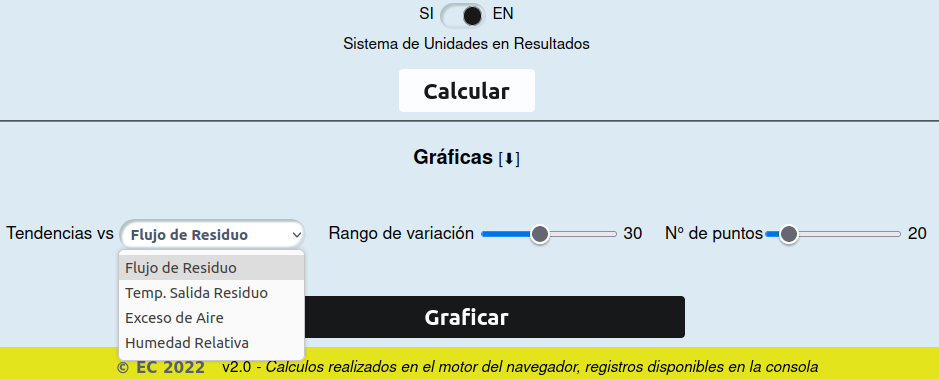
\includegraphics[scale=0.48]{images/curvas}
\caption[Opciones disponibles para graficar en el simulador]{Opciones disponibles para graficar en el simulador.}
\label{fig:curvas}\end{center}\end{figure}
\par Dependiendo del número de puntos escogidos por el usuario, el simulador podrá requerir más tiempo para finalizar los cálculos, en los rangos permitidos de la interfaz.
\par Definido un rango, este se divide entre un número de puntos establecido y se corre la simulación moviendo la variable escogida por cada punto.
\par Para observar y analizar los cambios generados se seleccionaron seis variables calculadas, a saber:
\begin{enumerate}
    \item El flujo de combustible.
    \item La temperatura de arco radiante.
    \item La temperatura de chimenea.
    \item La relación de absorción de calor entre las zona radiante y convectiva.
    \item La eficiencia térmica.
    \item Las emisiones de CO$_2$.
\end{enumerate}

\subsection{Variación de la carga del horno}
\par En la secuencia de Figuras \ref{fig:graph-t_out-fuel}, \ref{fig:graph-t_out-arc}, \ref{fig:graph-t_out-chim}, \ref{fig:graph-t_out-dist}, \ref{fig:graph-t_out-efic} y \ref{fig:graph-t_out-emi} se puede apreciar el cambio de las seis variables resultantes con la variación de la temperatura de salida del residuo (lo que es equivalente a aumentar la carga del horno), cuyas tendencias son equivalentes a aumentar el cantidad de fluido que circula.
\par En las gráficas de la interfaz del simulador se pueden observar puntos rojos representan los valores calculados por el simulador, unidos por una línea azul que dibuja la curva de la tendencia seleccionada; en el rango del eje de las abscisas se presenta la variable de entrada escogida.
\par En la Figura \ref{fig:graph-t_out-fuel}, se grafica el flujo de combustible variando la temperatura del fluido. Se observa el incremento el flujo de combustible necesario para cumplir con el aumento de la carga del horno.
\begin{figure}[H]\begin{center}
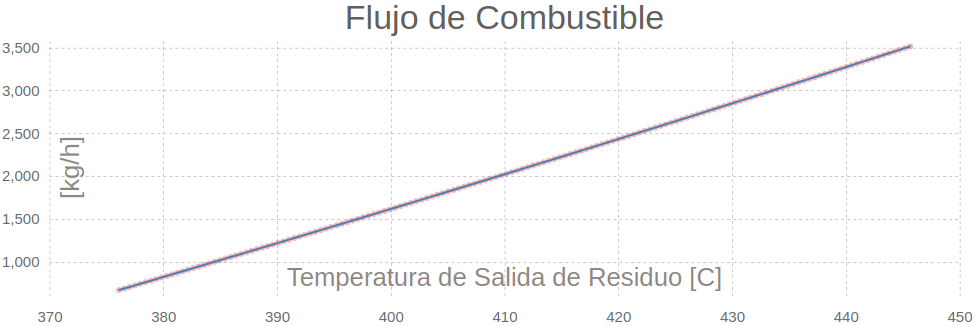
\includegraphics[scale=0.46]{images/graph-t_out-fuel}
\caption[Flujo de combustible en función de Temperatura de salida de residuo]{Flujo de combustible en función de la temperatura de salida de residuo.}
\label{fig:graph-t_out-fuel}\end{center}\end{figure}
\par Este comportamiento corresponde a que el combustible es la fuente de calor del horno y cualquier necesidad de energía adicional en el proceso requiere mayor flujo de combustible. Este comportamiento también se observa al aumentar el flujo de la carga, la humedad relativa y el exceso de aire, de forma independiente.
\par Al aumentar el flujo de combustible por el requerimiento de una temperatura de salida del fluido mayor, y manteniendo el resto de las variables de entrada, como exceso de aire y humedad relativa fijas, se nota un aumento en la temperatura de arco radiante (Fig. \ref{fig:graph-t_out-arc}) y, por consecuencia, en la temperatura de salida de los gases de chimenea (Fig. \ref{fig:graph-t_out-chim}).
\begin{figure}[H]\begin{center}
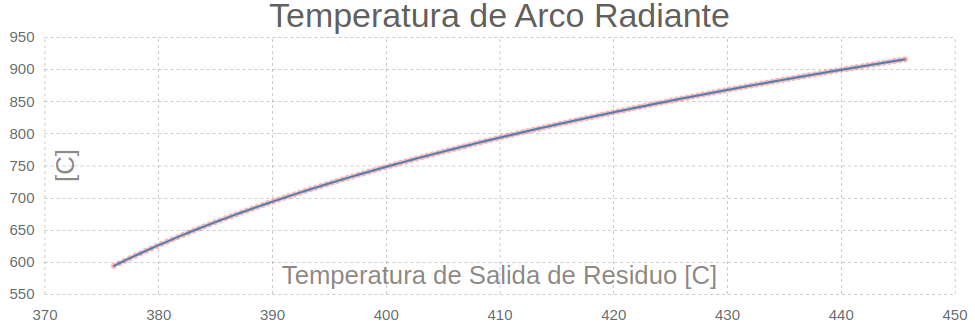
\includegraphics[scale=0.46]{images/graph-t_out-arc}
\caption[Temperatura de arco radiante en función de Temperatura de salida de residuo]{Temperatura de arco radiante en función de la temperatura de salida de residuo.}
\label{fig:graph-t_out-arc}\end{center}\end{figure}
\par El aumento observado en las Figuras \ref{fig:graph-t_out-fuel} y \ref{fig:graph-t_out-chim} se traduce en mas energía y gases de combustión liberados al ambiente, disminuyendo la eficiencia del horno y aumentado la contaminación generada por el proceso.
\begin{figure}[H]\begin{center}
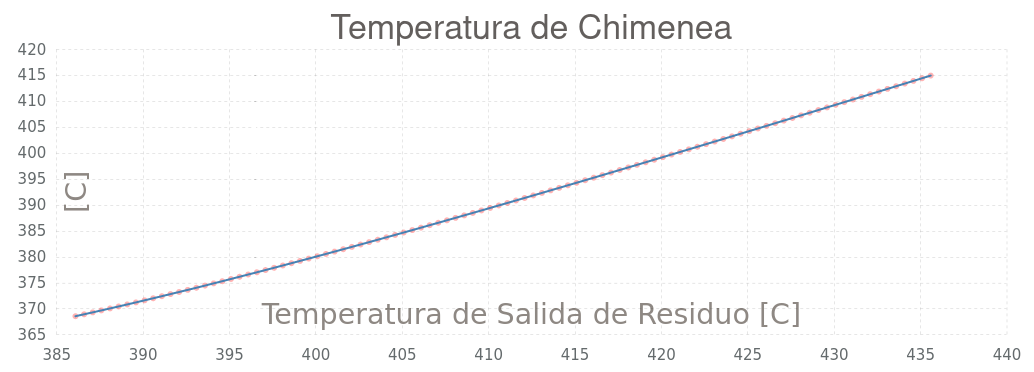
\includegraphics[scale=0.46]{images/graph-t_out-chim}
\caption[Temperatura de chimenea en función de Temperatura de salida de residuo]{Temperatura de chimenea en función de la temperatura de salida de residuo.}
\label{fig:graph-t_out-chim}\end{center}\end{figure}
\par Para la variable de la relación de calor absorbido por zona, la tendencia observada en la Figura \ref{fig:graph-t_out-dist} es decreciente, lo que se traduce en que el porcentaje de la absorción de calor disminuye en la zona radiante y aumenta en la zona convectiva, a pesar de que el calor transferido es siempre mayor en la zona radiante se debe considerar que están aumentando las pérdidas de calor por la chimenea.
\begin{figure}[H] \begin{center}
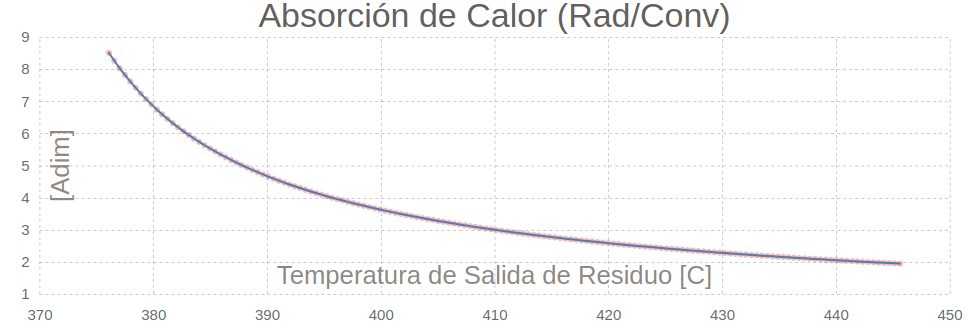
\includegraphics[scale=0.46]{images/graph-t_out-dist}
\caption[Distribución de absorción de calor en función de Temperatura de salida de residuo]{Tasa de distribución de absorción de calor entre zona radiante y convectiva en función de la temperatura de salida de residuo.}
\label{fig:graph-t_out-dist} \end{center} \end{figure}
\par Ambas zonas transfieren mayor cantidad de calor al fluido, pero la zona convectiva refleja un aumento porcentual mayor, proporcional a la temperatura de los gases de combustión, un factor a considerar es que la zona convectiva tiene un área de contacto casi diez veces mayor por la presencia de aletas.
\par La Figura \ref{fig:graph-t_out-efic} muestra la tendencia decreciente de la eficiencia térmica en función de la temperatura de salida del residuo. La tendencia refleja el incremento de las pérdidas de calor del horno como consecuencia de la menor absorción de calor en las secciones radiante y de escudo que no puede ser compensada por la sección convectiva. 
\begin{figure}[H]\begin{center}
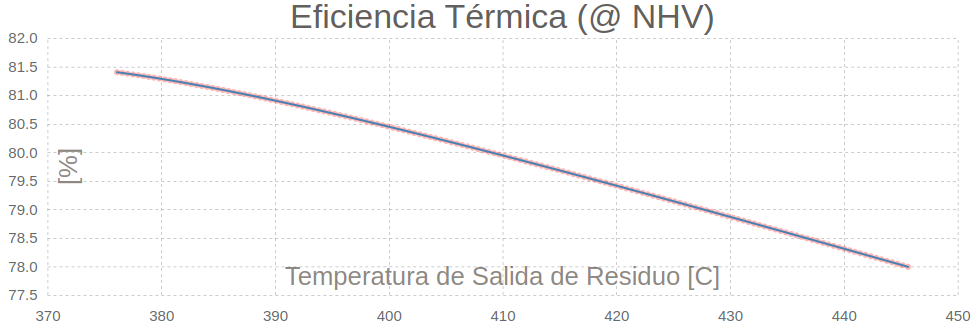
\includegraphics[scale=0.46]{images/graph-t_out-efic}
\caption[Eficiencia térmica en función de Temperatura de salida de residuo]{Eficiencia Térmica (@ Valor Calorífico Neto) en función de la temperatura de salida de residuo.}
\label{fig:graph-t_out-efic}\end{center}\end{figure}
\par Este comportamiento se observa también al aumentar las otras variables disponibles para este análisis, el exceso de aire, humedad y flujo de residuo, inversamente proporcional al aumento de la temperatura de los gases en la chimenea.
\par La Figura \ref{fig:graph-t_out-emi} muestra la tendencia ascendente de las emisiones de CO$_2$ con respecto a la temperatura de salida del residuo, lo cual, como ya se indicó, coincide con un mayor consumo de combustible y una disminución de la eficiencia térmica del horno.
\begin{figure}[H] \begin{center}
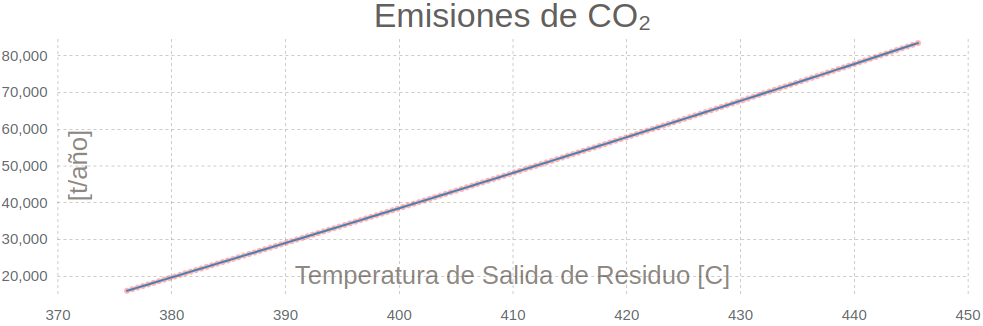
\includegraphics[scale=0.46]{images/graph-t_out-emi}
\caption[Emisiones de CO$_2$ en función de Temperatura de salida de residuo]{Emisiones de CO$_2$ en función de la temperatura de salida de residuo.}
\label{fig:graph-t_out-emi} \end{center} \end{figure}
\par Un comportamiento similar se observa para todas las variables estudiadas.

\subsection{Variación del exceso de aire y humedad relativa}
\par En la Figura \ref{fig:exceso-aire} se muestran las tendencias de las seis variables de salida en función al exceso de aire, agrupadas como se diseñó en el simulador, se observa el mismo comportamiento de aumento del flujo de combustible, temperatura de chimenea y emisiones de CO$_2$; y disminución de la eficiencia térmica y del porcentaje de absorción de calor en la zona radiante.
\par Observando que la única tendencia diferente es la correspondiente a la temperatura de arco radiante, que disminuye incluso al aumentar el flujo másico de los gases de combustión, a causa de que el calor generado ahora debe calentar una masa de aire adicional en la sección de radiación, como se aprecia en la ecuación \ref{eq:llama} de temperatura de arco radiante, descrita en la sección de combustión de hidrocarburos.
\begin{figure}[H] \begin{center} 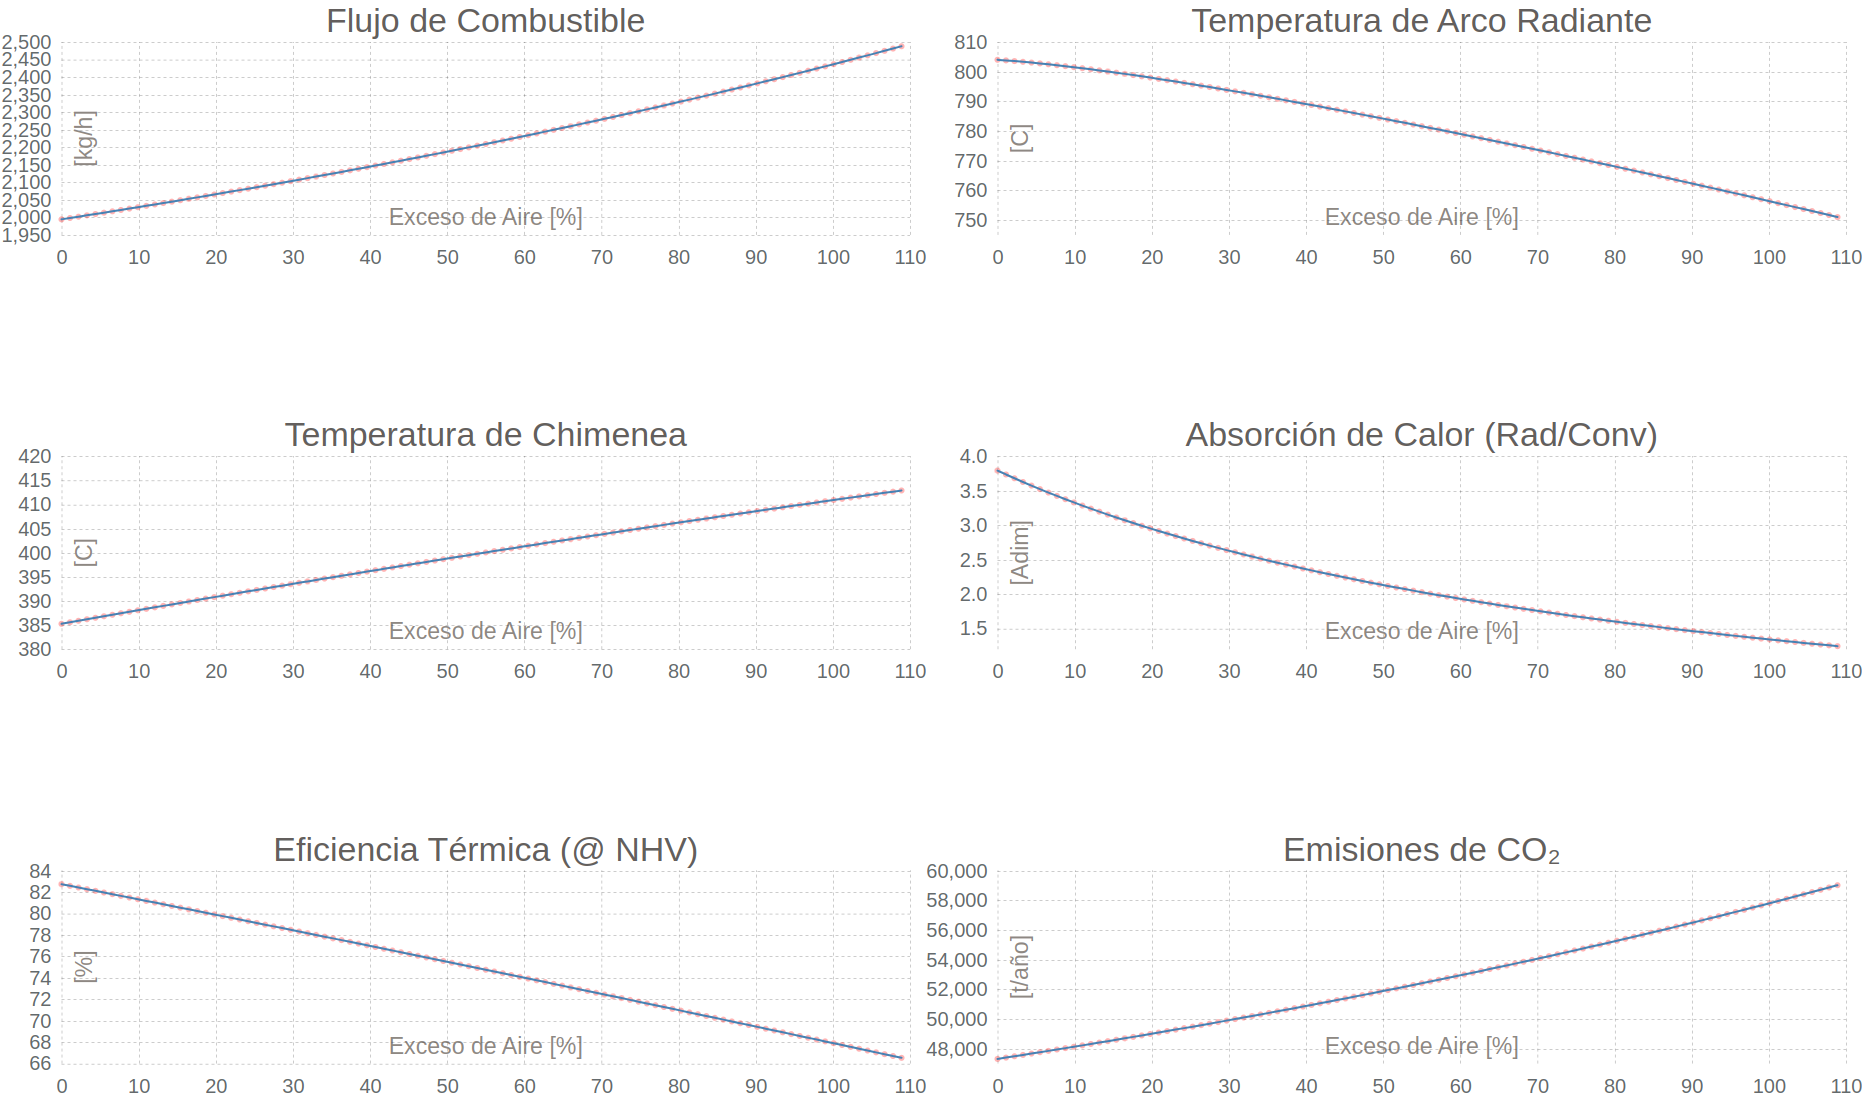
\includegraphics[scale=0.249]{images/exceso-aire}
\caption[Curvas de tendencia para la variación de exceso de aire]
{Curvas de tendencia para la variación de exceso de aire.}
\label{fig:exceso-aire} \end{center} \end{figure}
\par Comportamiento y tendencias similares se observan cuando se varia la humedad relativa en el aire de alimentación. Con lo que se tiene una referencia de la tendencia en todas las variables abiertas para graficar.

\section{Resultados del modo comparativo}
\par Este modo de la interfaz del simulador permite observar vis a vis los parámetros de dos condiciones de operación del horno, una condición Base y otra Modificada. Esta presentación posibilita comparar los cambios en las variables proceso y analizar las causas de los cambios registrados en los resultados operacionales.
\par En la Tabla \ref{tbl:comparison-cp} se observa un resumen de un caso Base, con las condiciones operacionales de diseño, y un caso Modificado en el cual el combustible (gas de refinería) contiene cuatro veces más hidrógeno, una menor proporción de hidrocarburos C1, C2 y C3, y, valores de poder calorífico ligeramente mayores.
\par La Tabla \ref{tbl:comparison-cp} contiene las condiciones operacionales del residuo atmosférico, los factores de ensuciamiento internos y externos de los tubos radiantes, del escudo y convectivos, las condiciones de combustión y la composición y las propiedades del combustible.
\begin{table}[H]
\caption{Condiciones de proceso del modo comparativo del simulador}
\label{tbl:comparison-cp} \centering \begin{tabular}{l|c|c}
\quad\quad\quad CASO    & BASE & MODIFICADO \\
\hline
\multicolumn{3}{c}{Residuo atmosférico} \\
Flujo volumétrico,  m$^3$/d   &14.309 &14.309 \\
Temperatura de entrada,  °C   &359    &359    \\
Temperatura de salida,  °C    &411    &411    \\
Gravedad específica           &0,84   &0,84   \\
Calor absorbido total,  MW    &20,862 &20,862 \\
\hline
\multicolumn{3}{c}{Factores de ensuciamiento} \\
Rfi (interno) radiante,  m$^2$-K/W 10$^{-3}$        &0,100  &0,100 \\
Rfi interno escudo/convectivo,  m$^2$-K/W 10$^{-3}$ &0,100  &0,100 \\
Rfo externo escudo/convectivo,  m$^2$-K/W 10$^{-3}$ &0,100  &0,100 \\
\hline
\multicolumn{3}{c}{Condiciones de combustión} \\
Exceso de aire, \%                      &20     &20   \\
Temperatura del aire de combustión, °C  &27     &27   \\
Humedad relativa, \%                    &50     &50   \\
Humedad del aire,  gH$_2$O/kg aire seco &11,107 &11,107\\
Pérdidas de calor al ambiente, \%       &1,5    &1,5  \\
\hline
\multicolumn{3}{c}{Características del combustible} \\
Metano (CH$_4$), \%          &56,47  &30,47  \\
Etano (C$_2$H$_6$), \%       &15,15  &8,15   \\
Propano (C$_3$H$_8$), \%     &6,22   &5,22   \\
n-Butano (C$_4$H$_{10}$), \% &1,76   &1,50   \\
i-Butano (C$_4$H$_{10}$), \% &0,75   &0,75   \\
Etileno (C$_2$H$_4$), \%     &1,58   &1,58   \\
Propileno (C$_3$H$_6$), \%   &2,77   &2,77   \\
Monóxido de carbono (CO), \% &0,66   &0,66   \\
Hidrógeno (H$_2$), \% &11,42&\colorbox{lightgray}{45,68}\\
Nitrógeno (N$_2$), \%        &0,68   &0,68   \\
Dióxido de carbono (CO$_2$), \%&2,54 &2,54   \\
\hline
Peso molecular,  kg/kmol               &21,149 &14,972 \\
Calor específico Cp (T comb),  kJ/kg-K &3,410  &7,595  \\
Poder Calorífico Neto (NCV),  kJ/kg    &45,718 &47,680 \\
Poder Calorífico Bruto (GCV),  kJ/kg   &50,268 &52,814 \\
\end{tabular}
\end{table}

\par En la Tabla \ref{tbl:comparison-r} se detallan uno a uno los resultados del caso Base y Modificado, de manera semejante a como se muestra en la interfaz web del simulador. Dentro de los resultados,vresaltan, la disminución del flujo de combustible en 3,5\% y, consecuentemente, de las emisiones de CO$_2$ en 10,8\%, lo que se debe directamente al incremento de la proporción de hidrógeno en el combustible para la operación modificada del horno, y, finalmente, el incremento de la eficiencia térmica.
\begin{table}[H]
\caption{Resultados del modo comparativo del simulador}
\label{tbl:comparison-r} \centering \begin{tabular}{l|c|c}
\quad\quad\quad CASO & BASE & MODIFICADO \\
\hline
\multicolumn{3}{c}{Flujos másicos,  kg/s} \\
Fluido de proceso (Residuo atmosférico)   &139,0         &139,0  \\
Combustible           &0,57 &\colorbox{lightgray}{0,55} \\
Aire                  &10,68         &10,38  \\
Gases de combustión   &11,28         &10,92  \\
\hline
(A/C) Masa BH        &18,693 &19,034 \\
(A/C) Volumen BH     &13,795 &9,944  \\
\hline
Suministro Térmico Combustible,  MW  &26,118 &25,999 \\
Suministro Térmico Total,  MW        &26,266 &26,169 \\
\hline
\multicolumn{3}{c}{Calor Absorbido,  MW}\\
Sección Radiante - (\%)  &13,099 - (62,79) &13,185 - (63,20)\\
Sección Escudo - (\%)    &3,311 - (15,87)  &3,313 - (15,88) \\
Sección Convectiva - (\%)&4,441 - (21,29)  &4,353 - (20,87) \\
\hline
Temperatura de pared (tubos radiantes), °C &434  &434  \\
Temperatura de Arco radiante, °C         &798  &798  \\
Temperatura de Chimenea, °C              &391  &391  \\
Temperatura Máxima Aletas (perímetro), °C &377  &376  \\
\hline
\multicolumn{3}{c}{Análisis de gases de combustión (Base Húmeda)}\\
CO$_2$, \%     &8,72    &7,93    \\
N$_2$, \%      &71,84   &71,23   \\
O$_2$, \%      &3,17    &3,14    \\
H$_2$O, \%     &16,27   &17,70   \\
\hline
Emisiones de CO$_2$, tonelada/año &48.790  &\colorbox{lightgray}{43.523} \\
\hline
\multicolumn{3}{c}{Pérdidas de calor,  MW}\\
Por chimenea - (\% del total)&4,888 - (18,61) &4,796 - (18,33) \\
Al ambiente - (\% del total) &0,392 - (1,49)  &0,390 - (1,49) \\
\hline
Eficiencia Térmica @ NHV, \%  &79,90 &80,18 \\
%Eficiencia Térmica @ GHV, \%  &72,70 &72,43 \\
\end{tabular} \end{table}
\par Esta comparación parte del supuesto de que el incremento del porcentaje de hidrógeno en el combustible puede ser manejado satisfactoriamente por los quemadores.

\par Otra comparación, resumida en la Tabla \ref{tbl:comparison-air}, al modificar únicamente el exceso de aire, de 20\% a 40\%, se observa: aumento en el consumo de combustible en 3,4\%, aumento en las emisiones de CO$_2$ en 3,6\%, aumento en el flujo de gases de combustión en 16,9\% y disminución en la eficiencia térmica de 2,9\%. 
\par Estos resultados se deben al consumo de energía térmica por parte del aire adicional suministrado al horno. Energía que no es transferida, subsiguientemente, al residuo atmosférico y que eventualmente se pierde por la chimenea. Evidenciando la importancia de esta variable en el proceso.
\begin{table}[H]
\caption{Resumen de comparación de aumento de exceso de aire en condiciones de diseño}
\label{tbl:comparison-air} \centering \begin{tabular}{l|c|c}
\quad\quad\quad CASO & BASE & MODIFICADO \\
\hline
\multicolumn{3}{c}{Condiciones de combustión} \\
Exceso de aire, \%      &20  &\colorbox{lightgray}{40}\\
Temperatura del aire de combustión, °C  &27     &27   \\
Humedad relativa, \%                    &50     &50   \\
Pérdidas de calor al ambiente, \%       &1,5    &1,5  \\
\multicolumn{3}{c}{Flujos másicos,  kg/s} \\
Fluido de proceso (Residuo atmosférico)   &139,0         &139,0  \\
Combustible           &0,57  &\colorbox{lightgray}{0,59} \\
Aire                  &10,68 & 12,93  \\
Gases de combustión   &11,28 &\colorbox{lightgray}{13,53}  \\
\hline
Exceso de oxígeno, \% (BH) &3,17   &5,50   \\
(A/C) Masa BH              &18,693 &21,809 \\
(A/C) Volumen BH           &13,795 &16,094  \\
\hline
Suministro Térmico Combustible,  MW  &26,118 &27,114 \\
\hline
Emisiones de CO$_2$, tonelada/año &48.790  &\colorbox{lightgray}{50.651} \\
\hline
\multicolumn{3}{c}{Pérdidas de calor,  MW}\\
Por chimenea - (\% del total)&4,888 - (18,61) &5,872 - (21,52) \\
Al ambiente - (\% del total) &0,392 - (1,49)  &0,407 - (1,49) \\
\hline
Eficiencia Térmica @ NHV, \%  &79,90 &\colorbox{lightgray}{76,99} \\
\end{tabular} \end{table}
\chapter*{Conclusiones}

%\begin{itemize}
    %\item 
    \par Se desarrollo exitosamente un modelo capaz de simular la operación de hornos de proceso, enfocado al adiestramiento de ingenieros y operadores, y con el objetivo de aumentar la eficiencia de estos equipos para disminuir el consumo de combustibles fósiles y generar menos gases de efecto invernadero.

    %\item 
    \par El modelo integra las ecuaciones de transferencia de calor y conservación de masa y energía en un algoritmo que simula el comportamiento estacionario de un horno de fuego directo, se comprobó su capacidad para generar resultados estables y confiables de las variables de proceso establecidas.
    
    %\item 
    \par El simulador para adiestramiento de hornos de proceso es una herramienta computacional de disposición pública y de código abierto, escrita en el lenguaje de programación JavaScript, que refiere parámetros confiables y prácticos para el uso académico o industrial dentro de las características mecánicas establecidas. El acceso directo se encuentra siguiendo el enlace (\url{https://e-usb.github.io/heater}).
    
    %\item 
    \par Los resultados generados por el simulador fueron validados aceptablemente mediante su comparación con un software comercial empleado para el diseño y evaluación termomecánica de hornos de proceso. Las tendencias de las variables operacionales simuladas mostraron resultados totalmente coherentes con la operación real de estos hornos en refinerías y plantas petroquímicas.

    %\item 
    \par Se incrementó el alcance del algoritmo desarrollado con la implementación de un modo comparativo y un modo de visualización de tendencias, aumentando las opciones de los usuarios al interactuar con el simulador.
%\end{itemize}
\chapter*{Recomendaciones}

\begin{itemize}
    \item El acceso a tecnologías libres que permitan desarrollar y continuar perfeccionando la simulación de procesos complejos, es aún muy limitada. De allí, nace la necesidad de establecer nuevos retos en los currículos de estudio para seguir facilitando los procesos de aprendizajes en la academia y en su posterior uso en la industria.
    
    \item Expandir las capacidades del simulador al incorporar caminos adicionales para el algoritmo, como el uso del flujo de combustible como una variable de entrada y hacer la temperatura de salida del fluido de residuo de vacío un resultado de la simulación.
    
    \item Añadir un camino en el algoritmo para incluir la opción de especificar el exceso de oxígeno en base seca para la combustión, ya que es común obtener este valor directamente de los medidores de oxígeno en hornos.
    
    \item Investigar a profundidad las consideraciones del tiro del horno y su relación con el movimiento del dámper en la chimenea, desarrollando ecuaciones que puedan acoplar estos conceptos con los fenómenos de transferencia de calor en el horno.
\end{itemize}
\nocite{*}
\bibliography{referencias}
\appendix
\chapter{Métodos iterativos}\label{apx:met}

\par En matemática computacional, un método iterativo trata de resolver un problema (como una ecuación o un sistema de ecuaciones) mediante aproximaciones sucesivas a la solución, empezando desde una estimación inicial. Esta aproximación contrasta con los métodos directos, que tratan de resolver el problema en un único intento (como resolver un sistema de ecuaciones Ax=b encontrando la inversa de la matriz A).
\par A modo de referencia se describen los métodos de aproximación de utilizados a continuación.

\section{Newton Raphson}
\par Es un algoritmo para encontrar aproximaciones de los valores iguales a ceros, o raíces, para una función de números reales. También puede ser usado para encontrar el máximo o mínimo de una función real, encontrando los puntos de inflexión, donde se iguala a cero su primera derivada, pero nuestro caso de enfoque será el mencionado inicialmente.
\par El método de Newton es un método abierto, en el sentido de que no está garantizada su convergencia global. La única manera de alcanzar la convergencia es seleccionar un valor inicial (semilla) lo suficientemente cercano a la raíz de la función buscada. Así, se ha de comenzar la iteración con un valor razonablemente cercano al cero (también denominado punto de arranque o valor supuesto). La relativa cercanía del punto inicial a la raíz depende mucho de la naturaleza de la propia función; si ésta presenta múltiples puntos de inflexión o pendientes grandes en el entorno de la raíz, entonces las probabilidades de que el algoritmo diverja aumentan, lo cual exige seleccionar un valor supuesto cercano a la raíz. Una vez que se ha hecho esto, el método linealiza la función por la recta tangente en ese valor supuesto. La abscisa en el origen de dicha recta será, según el método, una mejor aproximación de la raíz que el valor anterior. Se realizarán sucesivas iteraciones hasta que el método haya convergido a la tolerancia deseada o se alcanza el numero límite de iteraciones. 
\par Así como el valor inicial, el paso de cada iteración y la tolerancia, todas son variables que se ajustan a conveniencia en este método; los rangos de operación alcanzados por el simulador del horno dependerán en gran medida de estos valores.
\par El método se basa en el desarrollo de Taylor de la función cuya raíz se quiere calcular. Al considerar la ecuación $f(x)=0$, y suponiendo que posee una y sólo una solución $\alpha\in[a,b]$. Se parte de un punto $x_0$ suficientemente cercano a dicha raíz, se escribe:
\begin{equation*}
f(\alpha) = f(x_0)
    + (\alpha-x_0)f^\prime(x_0) 
    + \frac{\alpha-x_0}{2}f^{\prime\prime}(x_0+\theta h)
\end{equation*}
\par con $0<\theta<1$, $h=\alpha-x_0$.
\par Si se supone que $f^\prime(x)$ no se anula en $[a,b]$, y que la diferencia $\alpha-x_0$ es muy pequeña, el método de Newton-Raphson consiste en despreciar el sumando en $(\alpha-x_0)/2$ del desarrollo anterior, quedando con la aproximación:
\begin{equation*}
f(\alpha) \approx f(x_0) + (\alpha-x_0)f^\prime(x_0)
\end{equation*}
\par Como $\alpha$ es la solución de la ecuación $f(x)=0$, se tiene que $f(\alpha)=0$ y por tanto, de la expresión anterior se sigue que:
\begin{equation*}
f(x_0)+(\alpha-x_0)f^\prime(x_0) \approx 0
\end{equation*}
\par y despejando $\alpha$ resulta:
\begin{equation*}
\alpha \approx x_0 - f(x_0)f^\prime(x_0) = x_1
\end{equation*}
\par La implementación usada puede verse en los anexos donde se encuentra el código fuente del simulador.

\section{Bisección}
\par Se basa en el teorema del valor intermedio (TVI), el cual establece que toda función continua $f$ en un intervalo cerrado $[a,b]$ toma todos los valores que se hallan entre $f(a)$ y $f(b)$. Esto es que todo valor entre $f(a)$ y $f(b)$ es la imagen de al menos un valor en el intervalo $[a,b]$. En caso de que $f(a)$ y $f(b)$ tengan signos opuestos, el valor cero sería un valor intermedio entre $f(a)$ y $f(b)$, por lo que con certeza existe un  $p\in [a,b]$ que cumple  $f(p)=0$. De esta forma, se asegura la existencia de al menos una solución de la ecuación $f(x)=0$.
\par Es también un algoritmo de búsqueda de raíces o ceros en funciones reales, que trabaja dividiendo un intervalo dado a la mitad y seleccionando el subintervalo que tiene la raíz. Suele requerir más iteraciones para alcanzar la tolerancia deseada que el método Newton Raphson descrito anteriormente, además de conocer de antemano el intervalo donde se encuentra la raíz deseada, su ventaja es que en funciones continuas se puede garantizar su convergencia.
\chapter{EJEMPLO DE IMAGEN EN APÉNDICE}\label{apx:img}
\begin{figure}[ht]
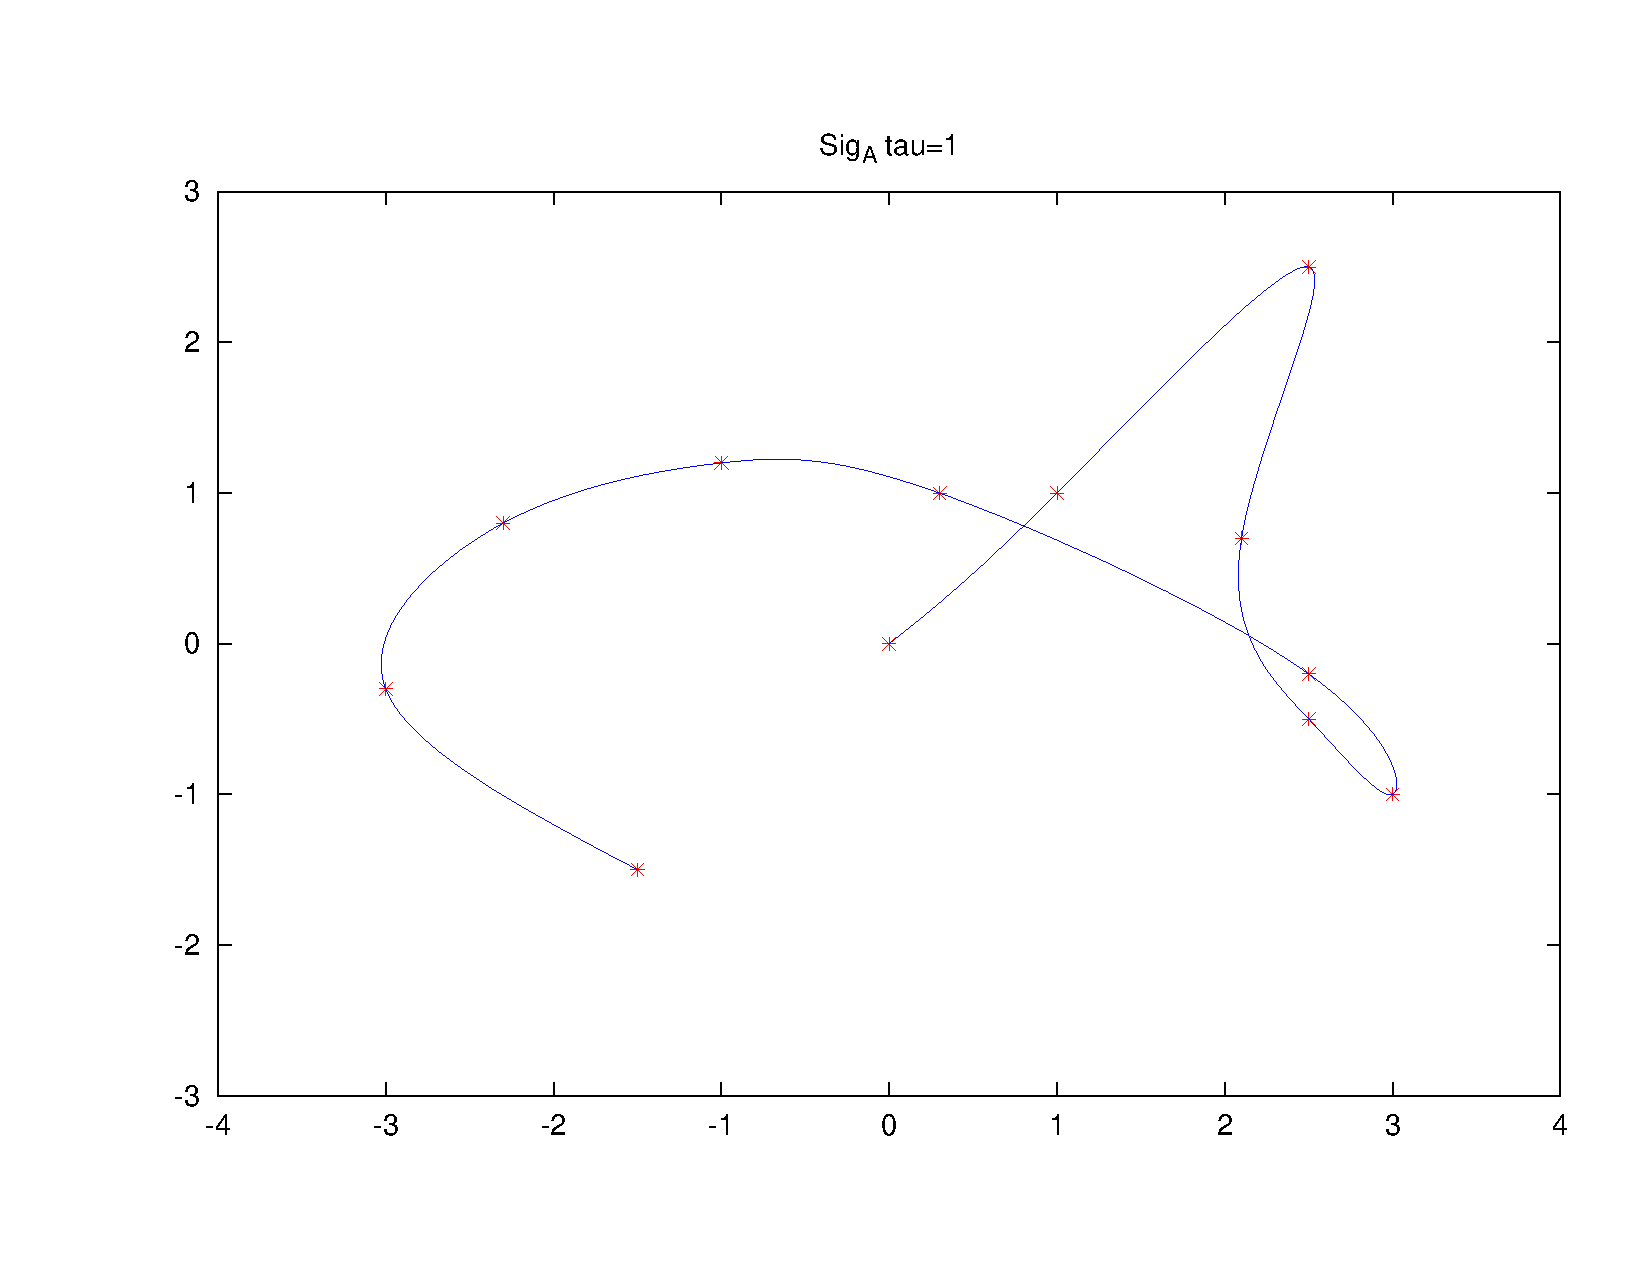
\includegraphics[scale=0.48,angle=0]{images/ejemplo}
\caption[Título corto de imagen]{Título corto de imagen}\label{img:imgscl}
\end{figure}



\chapter{Código desarrollado}

\par La versión organizada por archivos y carpetas se encuentra en el siguiente enlace \url{https://github.com/e-usb/heater}

\par El código usado únicamente para el algoritmo, sin incluir la interfaz, se muestra a continuación.

\section{Ciclo externo}

\begin{verbatim}
const { round, logger, options, unitConv, 
  initSystem, linearApprox, newtonRaphson, 
  viscosityApprox, kw_tubes_A312_TP321
} = require('./js/utils');
const data = require('./data/data.json');
const {radSection} = require('./js/heaterSections/rad');
const {convSection} = require('./js/heaterSections/conv');
const {shieldSection} = require('./js/heaterSections/shield');
const {combSection} = require('./js/heaterSections/combustion');
const {browserProcess} = require('./js/browser');

const createParams = (opts) => {
  const
    m_fluid = unitConv.BPDtolb_h(
      unitConv.lbtokg(opts.mFluid),
      opts.spGrav
    ), // kg/h
    t_in  = opts.tIn, // (K)
    t_out = opts.tOut,// (K)
    miu_fluid_in = opts.miuFluidIn,  // (cp)
    miu_fluid_out= opts.miuFluidOut, // (cp)
    cp_fluid_in  = opts.cpFluidIn, // (kJ/kg-C)
    cp_fluid_out = opts.cpFluidOut,// (kJ/kg-C) 
    kw_fluid_in = unitConv.kwENtokwSI(opts.kwFluidIn), // (kJ/h-m-C)
    kw_fluid_out= unitConv.kwENtokwSI(opts.kwFluidOut);// (kJ/h-m-C)

  return {
    runDistCycle: opts.runDistCycle,
    /** Inlet Amb Variables */
    p_atm:  opts.pAtm,         // (Pa) 
    t_fuel: opts.tFuel,        // (K) 
    t_air:  opts.tAir,         // (K)
    t_amb:  opts.tAmb,         // (K) ref
    humidity:  opts.humidity,  // (%) 
    airExcess: opts.airExcess, // (% *.01) 
    o2Excess:  opts.o2Excess,  // (% *.01) 
    
    /** Process Variables */
    sp_grav:   opts.spGrav, // -
    t_in_conv:  t_in,       // (K) global process inlet
    t_out:      t_out,      // (K) global process outlet
    m_fluid:    m_fluid,    // (kg/h) 
    Rfi:      opts.rfi,     // (h-m2-C/kJ) int. fouling rad
    Rfo:      opts.rfoConv, // (h-m2-C/kJ) ext. fouling cnv
    Rfi_conv: opts.rfiConv, // (h-m2-C/kJ) int. fouling conv sect
    Rfi_shld: opts.rfiShld, // (h-m2-C/kJ) int. fouling shld sect
    Rfo_shld: opts.rfoShld, // (h-m2-C/kJ) ext. fouling shld sect
    efficiency: opts.effcy,         // (% *.01)
    duty_rad_dist: opts.radDist,    // (% *.01)
    heat_loss_percent: opts.hLoss,  // (% *.01)
    max_duty: unitConv.BTUtokJ(71.5276*1e3),// (kJ/h) unused
    miu_fluid: viscosityApprox({
      t1: t_in,  v1: miu_fluid_in,
      t2: t_out, v2: miu_fluid_out
    }),                     // (cP)
    Cp_fluid: linearApprox({
      x1: t_in,  y1: cp_fluid_in,
      x2: t_out, y2: cp_fluid_out
    }),                     // (kJ/kg-C) 
    kw_fluid: linearApprox({
      x1: t_in,  y1: kw_fluid_in,
      x2: t_out, y2: kw_fluid_out
    }),                     // (kJ/h-m-C)
    
    /** Mechanic variables for heater */
    Material: 'A-312 TP321',
    h_conv: unitConv.hcENtohcSI(1.5),// (kJ/h-m2-C)
    kw_tube: kw_tubes_A312_TP321,    // (kJ/h-m-C)
    Pass_number: 2,          // - number of tube passes
    
    Pitch_rad: unitConv.intom(2*8),// (m) NPS * 2
    N_rad:  42,                    // - number of tubes 
    L_rad:  unitConv.fttom(62.094),// (m) tube effective length
    Do_rad: unitConv.intom(8.625), // (m) tube external diameter
    Sch_rad:unitConv.intom(0.322), // (m) Schedule thickness

    Burner_number: 13,            // - burner's number
    Do_Burner:   2.24,            // (ft) burner's outside diameter

    Width_rad:  17.50,            // (ft) width in rad sect
    Length_rad: 64.55,            // (ft) length in rad sect
    Height_rad: 27.00,            // (ft) height in rad sect
    
    N_shld: 16,                   // - number of tubes 
    L_shld: unitConv.fttom(60),   // (m) effective tube length
    Do_shld:unitConv.intom(6.625),// (m) external diameter 
    
    Pitch_sh_cnv: unitConv.intom(2*6),// (m) NPS * 2
    Sch_sh_cnv:  unitConv.intom(0.28),// (m) Schedule thickness
    Tpr_sh_cnv:  8,                   // - number of tubes per row

    N_conv: 40,                   // - number of tubes 
    L_conv: unitConv.fttom(60),   // (m) effective tube length
    Do_conv:unitConv.intom(6.625),// (m) external diameter 

    // Fin properties
    Nf:unitConv.mtoft(60),   // (#/m) Fin's number per meter
    Tf:unitConv.fttom(.005), // (m) Fin's thickness
    Lf:unitConv.fttom(0.08), // (m) Fin's height

    /** Miscellaneous */
    FinType: 'Solid',
    FinMaterial: '11.5-13.5Cr',
    FinArrange: 'Staggered Pitch',
    verbose: opts.verbose,       // True or False
    unitSystem: opts.unitSystem, // SI or English
    lang: opts.lang,             // EN or ES
    NROptions: opts.NROptions,   // {object options}
    units: initSystem(opts.unitSystem)
  }
}

const heaterFunc = (fuels, opts) => {
  const params = createParams(opts);

  // if params.o2Excess is set, start airExcess iteration
  if (params.o2Excess != 0) combustionCycle(params, fuels);

  const heat_result = combSection(params.airExcess, fuels, params);

  if (params.runDistCycle) externalCycle(params);

  heat_result.rad_result = radSection(params);
  heat_result.shld_result = shieldSection(params);
  heat_result.conv_result = convSection(params);
  heat_result.rad_result.eff_thermal_val = 
    heat_result.rad_result.eff_thermal(heat_result.conv_result.Q_stack);
  heat_result.rad_result.eff_gcv_val = 
    heat_result.rad_result.eff_gcv(heat_result.conv_result.Q_stack);

  return heat_result
}

const externalCycle = (params) => {
  // cycle iter count and flag for debugging logs 
  let cycle = 0, noLog = true;
  const rad_dist = (radDist) => {
    cycle++;
    if (radDist >0.3 && radDist <1) {
      params.duty_rad_dist = radDist;
    }
    const int_rlt = {
      rad:  radSection(   params, noLog),
      shld: shieldSection(params, noLog),
      conv: convSection(  params, noLog)
    };
    const duty_calc = Math.abs(int_rlt.rad.Q_fluid) + 
    Math.abs(int_rlt.shld.Q_fluid) + Math.abs(int_rlt.conv.Q_fluid);

    return (params.duty - duty_calc)/duty_calc;
  };
  const convNROptions = {...params.NROptions};
  convNROptions.maxIterations *= 5;
  convNROptions.tolerance *= 1e-1;
  convNROptions.epsilon *= 1e-1;
  convNROptions.h *= 1e-1;
  const rad_dist_final = newtonRaphson(rad_dist, 
    params.duty_rad_dist, convNROptions, 'rad_dist_final');
  if (rad_dist_final >0.1 && rad_dist_final <1) { 
    params.duty_rad_dist = rad_dist_final; 
  } else {
    logger.error('external cycle broken, error in rad_dist estimation, using: '+
    params.duty_rad_dist);
  }
  logger.info(`duty_rad_dist: ${
    round(100*rad_dist_final,2)}, ext_cycle_reps: ${cycle}`);
}

const combustionCycle = (params, fuels) => {
  // cycle iter count and flag for debugging logs 
  let cycle = 0, onlyO2 = true;
  const comb_o2 = (airExcessVal) => {
    cycle++;
    const combO2 = combSection(airExcessVal, fuels, params, onlyO2)
    if (!onlyO2) logger.info( `'O2%_comb': ${combO2.flows['O2_%']}, `+
      `O2excess: ${params.o2Excess *100}`);

    return Math.round(combO2.flows['O2_%']*1e5 -params.o2Excess*1e7);
  }
  const convNROptions = {...params.NROptions};
  convNROptions.maxIterations *= 5;
  convNROptions.tolerance *= 1e-1;
  convNROptions.epsilon *= 1e-1;
  convNROptions.h *= 1e-1;
  const airExcess = newtonRaphson(comb_o2,.05,
    convNROptions, 'o2_excess_to_air');

  if (airExcess) params.airExcess = airExcess;
  logger.info(`'air_excess': ${round(100*airExcess,2)}, `+
    `'comb_cycle_reps': ${cycle}`);
}

let fuelsObject = { 
  H2:     .1142, N2:   .0068, CO:   .0066, CO2: .0254, 
  CH4:    .5647, C2H6: .1515, C3H8: .0622, C4H10: .0176, 
  iC4H10: .0075, C2H4: .0158, C3H6: .0277,
};
// Fuel for debugging purpose
// fuelsObject ={
//   CH4: 1,
//   // H2: .7, O2: .2, N2: .1
// };

/** App entry point */
if (typeof window !== 'undefined') {
  browserProcess(fuelsObject, data, options, heaterFunc)
} else {
  logger.info(JSON.stringify(heaterFunc(fuelsObject, options), null, 2))
}
\end{verbatim}

\subsection{Combustión}
\begin{verbatim}
const { newtonRaphson, options, logger,
  round, roundDict, initSystem,
  normalize, flueViscosity, flueThermalCond
} = require('../utils');
const data = require('../../data/data.json');
const dryAirN2Percentage = 79.05;
const dryAirO2Percentage = 20.95;
const N2O2relation = dryAirN2Percentage/dryAirO2Percentage;
const dryAir = {
  O2: .01 * dryAirO2Percentage,
  N2: .01 * dryAirN2Percentage,
  H2O: 0
};

/** Check if the percentages of the fuels sums 100%.
 * In case of check fail an error will be attached to the result.
*/
const checkObjectFraction = (fuels, result = {}) => {
  const total = Object.values(fuels).reduce((acc, value)=> acc + value)
  const tolerance = 3e-12
  const check1 = Math.abs(1 - total) <= tolerance
  if (!check1) result.err += `[fuel fraction not equal to 1,` + 
    ` total: ${total}. fuels: ${Object.keys(fuels)}],`;
  return check1;
};

/** Check if all the components in the fuels are in the data filtered.
 * In case of a bad fuel entered an error will be attached to the result.
*/
const checkFuelData = (fuels, compounds, result = {}) => {
  const badFuels = Math.abs(compounds.length - 
    Object.keys(fuels).length);
  const check1 = badFuels === 0;
  if (!check1) {
    logger.error(`[some fuels aren't in the database, #badFuels: ${badFuels}],`);
    result.err += `[some fuels aren't in the database, #badFuels: ${badFuels}],`;
  }
  return check1;
};

/** (kJ/kg K) to call returning function use Kelvin units 
  * if you want a result in (kJ/kmol K) units, multiply the
  * result by MW or call this with second argument set to true.
 */
const Cp0 = ({c0, c1, c2, c3, MW, Substance}, molResult, noLog) => {
  // Cp equation from table A.6 Van Wylen
  // Teta = T(Kelvin)
  return (teta) => {
    // Approximate equation valid from 250 K to 1200 K.
    if (teta < 250 && !noLog) logger.debug(`"Cp0", "temp": "${round(teta)}",`+
      `"Msg": "${Substance} bellow range for Cp0 formula"`);
    if (teta > 1200&& !noLog) logger.debug(`"Cp0", "temp": "${round(teta)}",`+
      `"Msg": "${Substance} above range for Cp0 formula"`);
    if (c0 === "-") {
      logger.debug(`"Cp0", "Msg": "Wrong use, called for compound `+
      `${Substance}, no data found"`);
      return 0;
    }
    if (molResult) return MW*(c0 + c1*(teta*.001) + 
        c2*(teta*.001)**2 + c3*(teta*.001)**3)
    return (c0 + c1*(teta*.001) + c2*(teta*.001)**2 + c3*(teta*.001)**3)
  }
};

/** (kJ/kg K) argument needs to be a fuel object,
* ie: { CH4: 0.323, ... }
* if you want a result in (kJ/kmol K) units, call it with 
* second argument set to true.
*/
const Cp_multicomp = (fuels, molResult, noLog) => {
  if (fuels.length === 0) return (_t) => 0
  // making a deep copy and normalize if needed
  let normalFuel = JSON.parse(JSON.stringify(fuels));
  if (!checkObjectFraction(fuels)) 
    normalFuel = normalize(normalFuel, "Cp_multicomp", noLog);
  const fuelComps = data.filter(elem => elem.Formula in normalFuel);
  const cps = [];
  let i = 0;
  for (const fuel in normalFuel) {
    cps[i] = (t) => normalFuel[fuel] * Cp0(
      fuelComps.filter(elem => elem.Formula == fuel)[0], molResult
    )(t);
    i++;
  }
  
  return cps.reduce((acc, val) => ((t) => acc(t) + val(t)), (_t) => 0);
};

/** (kg/kmol) argument needs to be a fuel object,
* ie: { CH4: 0.323, ... }
*/
const MW_multicomp = (fuels, noLog) => {
  if (fuels.length === 0) return (_t) => 0;
  // making a deep copy and normalize if needed
  let normalFuel = JSON.parse(JSON.stringify(fuels));
  if (!checkObjectFraction(fuels)) 
    normalFuel = normalize(normalFuel, "MW_multicomp", noLog);
  const fuelComps = data.filter(elem => elem.Formula in normalFuel);
  let MWs = 0;
  for (const fuel in normalFuel) {
    MWs += fuelComps.filter(elem => elem.Formula == fuel)[0].MW * 
    normalFuel[fuel];
  }
  return MWs;
};

/** (Pa) Temperature should be in K, humidity %[0,100] */
const pressureH2OinAir = (temperature, relativeHumidity) => {
  // Equation from Reference: Tetens, O., 1930

  // This eq uses temp in °C
  const temp = temperature - options.tempToK;
  // ps is the saturation vapour pressure, in pascals,
  const ps = 610.78*Math.exp(temp/(temp+238.3)*17.2694);
  // result pw is the actual water vapour pressure.
  return ps * relativeHumidity * 0.01;
};

/** Temperature should be in K, humidity %[0,100] */
const moistAirWeightRatio = (temperature, relativeHumidity) => {
  const pw = pressureH2OinAir(temperature, relativeHumidity)
  // returned value is the weight ratio of water vapour and dry air.
  // (kg-w_vap/kg-dry_a)
  return data[31].MW * pw / 
  ( MW_multicomp(dryAir) * (options.pAtm - pw ) );
  // a simplification can be: 0.62 * 1e-5 * pw
  
  /* weight ratio converted to water per oxygen in air
  const w = data[31].MW * pw / 
    ( MW_multicomp(dryAir) * (options.pAtm - pw ) );
  return w * 7.655;
  //*/
};

/** (kJ/kmol), Enthalpy of formation plus delta enthalpy 
  * returns a function if no temp is passed */
const deltaH = (compound, t) => {
  if (compound.Cp0 === '-') {
    if (compound.h0 === '-') {
      logger.warn(`wrong use of deltaH func,`+
        ` called for compound ${compound.Substance} without data`);
      if (t === undefined) return () => 0;
      return 0;
    }
    if (t === undefined) return () => compound.h0
    return compound.h0;
  }
  // hf0 + deltaH(tempAmbRef -> t)
  if (t === undefined) return (temp) => compound.h0 +(temp-options.tempAmbRef)*
    Cp0(compound,true, true)((options.tempAmbRef+temp)/2);

  return compound.h0 + (t-options.tempAmbRef)*
    Cp0(compound,true, true)((options.tempAmbRef+t)/2);
};

/** (kJ/kmol), Enthalpy of combustion for a certain compound 
  * returns a function if no temp is passed */
const combustionH = (compound, t, tIni, liquidWater = false) => {
  // hrp = HP - HR // H = H0 + deltaH  // H0 = n(hf)
  // SR ni*(hf + deltaH)i = SP ne*(hf + deltaH)e

  const 
    co2_H = deltaH( data[6]  ),
    so2_H = deltaH( data[34] ),
    o2_H  = deltaH( data[2]  );
  let h2o_H = deltaH(data[31]); // gas lower heating value 
  // higher heating value
  if (liquidWater === true) h2o_H = deltaH(data[32]); // liq
  // making tIni equal to t_amb if not specified
  if (tIni === undefined) tIni = options.tAmb;

  if (t === undefined) return (tempParam) => compound.CO2*co2_H(tempParam) 
    + compound.SO2*so2_H(tempParam) +compound.H2O*h2o_H(tempParam)
    - deltaH(compound)(tIni) - compound.O2*o2_H(tIni);
  
  // SR ni*(hf + deltaH)i = SP ne*(hf + deltaH)e
  return ( compound.CO2*co2_H(t) +compound.SO2*so2_H(t) +compound.H2O*h2o_H(t)
    - deltaH(compound)(tIni) - compound.O2*o2_H(tIni) );
};

/** (kJ/kg) Enthalpy of combustion for a certain fuel mix */
const ncv = (fuels, products, compounds, tAmb, gcv = false) => {
  let value = 0;
  for (const fuel in fuels) {
    if (fuel in products) continue;
    const compound = compounds.filter(elem => elem.Formula == fuel)[0]
    value += fuels[fuel]*combustionH(compound, undefined, tAmb, gcv)(tAmb);
    //logger.info(`H of combustion for ${fuel}: ` +
    // `${combustionH(compound)(tAmb)/compound.MW} KJ/Kg` )
  }
  return value;
};

/**Temp unit (K)
* Internal units (kJ/kmol)
* Function to create the adiabatic flame equation 
* used in the newton raphson method to find adFlame temp */
const adFlame = (normalFuels, products, tIni, o2required) => {
  if (tIni === undefined) tIni = options.tAmb;
  if (o2required === undefined) o2required = 0;
  const 
    fuelCompounds = data.filter(elem => elem.Formula in normalFuels),
    // ..._H = (t) => hf0 + MW * Cp(t_prom) * (t - t_amb)
    o2_H =  deltaH(data.filter(elem => elem.Formula == "O2")[0]),
    n2_H =  deltaH(data.filter(elem => elem.Formula == "N2")[0]),
    co2_H = deltaH(data.filter(elem => elem.Formula == "CO2")[0]),
    h2o_H = deltaH(data.filter(elem => elem.Formula == "H2O")[0]),
    so2_H = deltaH(data.filter(elem => elem.Formula == "SO2")[0]);

  // Products enthalpy at the new temp minus dry air inlet
  const pEnthalpy = (t) => products.O2*o2_H(t) + products.SO2*so2_H(t) +
    products.H2O*h2o_H(t) + products.CO2*co2_H(t) + 
    products.N2*n2_H(t) - products.N2*n2_H(tIni) - o2required*o2_H(tIni);
  
  // Reactants enthalpy (fuel)
  const rEnthalpy = [];
  let i = 0;
  for (const fuel in normalFuels) {
    // fuelFraction * [hf0 + MW * Cp(t_prom) * (tIni - t_amb)]
    rEnthalpy[i] = normalFuels[fuel]*deltaH(
      fuelCompounds.filter(elem => elem.Formula == fuel)[0]
    )(tIni);
    i++;
  }
  
  // SR ni*(hf + deltaH)i = SP ne*(hf + deltaH)e
  return (t) => pEnthalpy(t) - rEnthalpy.reduce((acc, value)=> acc + value);
};

/** For every element in the fuel compounds 
 * calculates every product of combustion per fuel element
 * filling the product object.
*/
const combPerFuelCompound = (compounds, products, normalFuel) => {
  for (const elem of compounds) {
    for (const product in products) {
      if (product == 'N2') {
        if (elem['Formula'] == 'N2' || elem['Formula'] =='"N2a') {
          products[product] += normalFuel[elem['Formula']];
          continue;
        }
        products[product] += elem['O2']*normalFuel[elem['Formula']]*N2O2relation;
        continue;
      }
      products[product] += elem[product]*normalFuel[elem['Formula']];
      // logger.default(`${elem['Formula']} req = ${product} ` +
      //   `${elem[product]*normalFuel[elem['Formula']]}` )
    }
  }
}

/** In this process the params object will be updated
*  in every function call with the combustion data
*/
const combSection = (airExcess, fuels, params, onlyO2) => {
  if (!onlyO2) logger.debug(`"airExcess", "value": ${airExcess}`);
  const units = initSystem(params.unitSystem);
  const moisture_val = moistAirWeightRatio(
    params.t_air, params.humidity
  );
  const debug_data = {
    err: "",
    atmPressure:     units.pressure(params.p_atm),
    fuelTemperature: units.tempC(params.t_fuel,0),
    ambTemperature:  units.tempC(params.t_amb,0),
    airTemperature:  units.tempC(params.t_air,0),
    "humidity_%": params.humidity,
    "dryAirN2_%": round(dryAirN2Percentage,2),
    "dryAirO2_%": round(dryAirO2Percentage,2),
    moisture:   units.moist(moisture_val),
    spGrav: params.sp_grav,
    cpFluidTb: units.cp(params.Cp_fluid((params.t_in_conv + params.t_out) /2)),
    unitSystem: units.system[params.lang]
  };
  const compounds = data.filter((elem, _i, _arr) => elem.Formula in fuels)

  let normalFuel = {...fuels};
  if (!checkObjectFraction(fuels, debug_data)) 
    normalFuel = normalize(fuels, "combSection");
  checkFuelData(normalFuel, compounds, debug_data);

  const products = {O2:0, N2:0, H2O:0, CO2:0, SO2:0}, air = {...dryAir};

  // filling products object with stoichiometric ratio
  combPerFuelCompound(compounds, products, normalFuel);

  // air excess and humidity shouldn't be less than 0
  if (airExcess - 0.000001 < 0) airExcess = 0;
  if (params.humidity - 0.000001 < 0) params.humidity = 0;
  /** Percentage of O2 in excess = 100% + x% airExcess */
  let o2required = products['O2'];
  let o2excess = o2required * (1 + airExcess);
  // If O2 requirements are negative 
  if (products['O2'] <= 0 || products['N2'] < 0) {
    logger.error(`airExcess set to 0, O2 in fuel >= O2 needed.`+
    ` Products: {O2:${products['O2']}, N2:${products['N2']}}`);
    o2excess   = 0;
    o2required = 0;
    products['N2'] = normalFuel['N2'];
    products['O2'] = -products['O2'];
  } else {
    const 
      waterPressure  = pressureH2OinAir(params.t_air, params.humidity),
      dryAirPressure = params.p_atm - waterPressure;
    air.N2  = .01* dryAirN2Percentage* dryAirPressure / params.p_atm;
    air.O2  = .01* dryAirO2Percentage* dryAirPressure / params.p_atm;
    air.H2O = waterPressure / params.p_atm;
    
    debug_data.dryAirPressure = units.pressure(dryAirPressure);
    debug_data.waterPressure  = units.pressure(waterPressure);
    debug_data["H2OPressure_%"] = round(100 * air.H2O);
    debug_data["N2Pressure_%"]  = round(100 * air.N2);
    debug_data["O2Pressure_%"]  = round(100 *air.O2);

    products['O2'] = o2excess -products['O2']; // Subs O2 used in combustion
    products['N2']  += products['O2']*(air.N2/air.O2);
    products['H2O'] += products['N2']*(waterPressure/(air.N2*params.p_atm));
  }

  let totalPerMol = 0, totalPerM_Dry = 0;
  for (const product in products) {
    totalPerMol += products[product];
    if (product !== 'H2O') totalPerM_Dry += products[product];
  }
  const flows = {
    total_flow: totalPerMol,
    dry_total_flow: totalPerM_Dry,
    // 'O2%_DRY': 100*products['O2'] /totalPerM_Dry,
    // 'CO2%_DRY':100*products['CO2']/totalPerM_Dry,
    // 'N2%_DRY': 100*products['N2'] /totalPerM_Dry,
    'N2_%': 100*products['N2'] /totalPerMol,
    'H2O_%':100*products['H2O']/totalPerMol,
    'CO2_%':100*products['CO2']/totalPerMol,
    'O2_%': 100*products['O2'] /totalPerMol,
    
    moisture_val,

    O2_mol_req_theor: o2required,
    O2_mass_req_theor:units.mass(o2required * data[2].MW),
    'air_excess_%':   100 * params.airExcess,
    AC:               o2excess / air.O2,
    AC_theor_dryAir:  o2required / (.01 * dryAirO2Percentage),
    AC_mass:          o2excess / air.O2 * 
      MW_multicomp(air)/MW_multicomp(normalFuel),
    AC_mass_theor_moistAir: o2required / air.O2 * 
      MW_multicomp(air)/MW_multicomp(normalFuel),

    fuel_MW: MW_multicomp(normalFuel),
    Cp_fuel: Cp_multicomp(normalFuel),

    flue_MW: MW_multicomp(products,onlyO2),
    Cp_flue: Cp_multicomp(products,false,onlyO2)
  };

  if (onlyO2) return {flows, products, debug_data};

  /** Adding results in parameters to be used in following sections */

  params.m_flue_ratio = totalPerMol * flows.flue_MW/MW_multicomp(normalFuel);  
  // kg/h
  params.m_air_ratio  = o2excess / air.O2 *
  MW_multicomp(air)/MW_multicomp(normalFuel); // kg/h

  params.Pco2 = products['CO2']/totalPerMol; // fraction
  params.Ph2o = products['H2O']/totalPerMol; // fraction

  // Functions of temp (kJ/kg-K)
  params.Cp_air  = Cp_multicomp(air);
  params.Cp_fuel = Cp_multicomp(normalFuel);
  params.Cp_flue = flows.Cp_flue;
  params.miu_flue= flueViscosity( data, products );
  params.kw_flue = flueThermalCond(data, products);
  flows.Cp_fuel_val  = flows.Cp_fuel(params.t_fuel);
  flows.Cp_fuel  = units.cp(flows.Cp_fuel_val);
  flows.Cp_flue  = units.cp(flows.Cp_flue(params.t_air));
  flows.flue_MW  = units["mass/mol"](flows.flue_MW);

  params.NCV = -ncv(normalFuel, products, compounds, params.t_amb)/
  MW_multicomp(normalFuel); // kJ/kg
  params.GCV = -ncv(normalFuel, products, compounds, params.t_amb, true)/
  MW_multicomp(normalFuel); // kJ/kg
  flows.NCV = units["energy/mass"](params.NCV,0);
  flows.GCV = units["energy/mass"](params.GCV,0);
  flows.NCV_val = params.NCV;
  flows.GCV_val = params.GCV;

  params.adFlame = newtonRaphson(
    adFlame(normalFuel, products, params.t_amb, o2excess),
    2000, params.NROptions, "fuel_adFlame");
  logger.info( `Adiabatic flame temp: [${round(params.adFlame)} K]`+
    ` ${units.tempC(params.adFlame)}`);

  roundDict(products);
  if (debug_data.err == "") delete debug_data.err;
  return {flows, products, debug_data};
};

module.exports = {
  combSection
};
\end{verbatim}

\subsection{Zona Radiante}
\begin{verbatim}
const {newtonRaphson, logger, round, unitConv} = require('../utils');

/** radSection receives the parameters dictionary and
 * calculates the required mass fluid or the necessary
 * temperature change at the radiant section.
 * 
 * First assumption to start the calc is duty transferred
 * in radiant section = 70% of total duty
 * 
 * Q_in = Q_rls + Q_air + Q_fuel =
 * Q_out = Q_R + Q_shield + Q_losses + Q_flue
 * Q_in(tg_out) - Q_out(tg_out) ~= 0
 * 
 * Q_rad + Q_conv = Q_R = Q_fluid(out-in)
*/
const radSection = (params, noLog) => {
  /** There are two starting cases A & B
   * Case A: given the fluid temp at the exit point of heater.
   * Case B: given the flow mass of the fuel at the heater burners. 
   * */
  let 
    tg_out = 0, // (K) Leaving/effective gas temp
    t_in   = 0, // (K) Inlet fluid temp
    t_out  = params.t_out,  // (K) Outlet fluid temp
    m_fuel = params.m_fuel; // (kg/h)

  let 
    duty_total  = 0, // (kJ/h) Duty in the hole fired heater
    duty_rad = 0; // (kJ/h) Duty in the radiant section
  
  const // Temperatures
    t_air     = params.t_air,    // (K) Inlet air temp
    t_fuel    = params.t_fuel,   // (K) Inlet fuel temp
    t_amb     = params.t_amb,    // (K) Ambient temp
    t_in_conv = params.t_in_conv,// (K) Heater inlet fluid temp
    /** (K) bulk temp (second arg default to rad inlet fluid temp) */
    Tb = (tOut, tIn = t_in) => 0.5*(tIn + tOut);

  const // Fired heater parameters
    Rfi = params.Rfi,      // (h-m2-C/kJ) internal fouling factor
    N = params.N_rad,      // (-) number of tubes in rad sect
    N_shld = params.N_shld,// (-) number of tubes in shld sect
    L = params.L_rad,      // (m) effective tube length
    L_shld = params.L_shld,// (m) effective tube length
    Do = params.Do_rad,    // (m) external diameter rad section
    Di = params.Do_rad - params.Sch_rad,// (m) int diameter rad sect
    S_tube = params.Pitch_rad || 0.394, // (m) center to center distance of tube
    S_tube_shld = params.Pitch_sh_cnv,    // (m) center to center distance of tube
    h_conv = params.h_conv || 30.66, 
    // (kJ/h-m2-C) Film convective heat transfer coff

    /** (ft) Mean Beam Length, dim ratio 1-2-1 to 1-2-4*/
    MBL = (2/3)*(params.Width_rad*params.Length_rad*params.Height_rad)**(1/3),
    PL  = (params.Ph2o + params.Pco2) * MBL, // atm-ft
    alpha = 1 +.49*(S_tube/Do)/6 -.09275*(S_tube/Do)**2 +
        .065*(S_tube/Do)**3/6 +.00025*(S_tube/Do)**4,
    alpha_shld =  1, // (-) alpha shield factor
    
    At = N *Math.PI *Do *L, // (m2) Bank tube's external surface area
    Acp = N * S_tube * L,   // (m2) Cold plane area of radiant tube bank
    Acp_shld = N_shld/2 *S_tube_shld*L_shld, 
    // (m2) Cold plane area of shield tube bank
    Ar = Ar_calc(params),   // (m2) Total refractory area
    {Aw, Aw_aAcp} = Aw_calc(alpha, Acp, alpha_shld, Acp_shld, Ar), // (m2)
    Ai = Math.PI*(Di**2)/2, // (m2) Tube's inside flux area x2
    cnv_fact = 3_600 *1e-3, // (g/s -> kg/h) secondsToHours * 1/k

    sigma = 5.670374e-8 *cnv_fact, // (W/m2-K4) -> (kJ/h-m2-K4)
    F = (temp) => effectivity(
        PL, alpha, Acp, alpha_shld, Acp_shld, Ar)(unitConv.KtoF(temp));

  const // Process Variables
    duty_rad_dist = params.duty_rad_dist         || .7,   // (-) % *.01
    efficiency = params.efficiency               || .8,   // (-) % *.01
    heat_loss_percent = params.heat_loss_percent || .015, // (-) % *.01
    NCV = params.NCV, // (kJ/kg) net calorific value
    GCV = params.GCV, // (kJ/kg) net calorific value
    m_fluid= params.m_fluid, // (kg/h) Fluid mass flow
    m_air  = (mFuel = m_fuel) => params.m_air_ratio*mFuel, // (kg/h) Air mass flow
    m_flue = (mFuel = m_fuel) => params.m_flue_ratio*mFuel,// (kg/h) Flue mass flow
    Cp_fuel = params.Cp_fuel(Tb(t_fuel, t_amb)), // (kJ/kg.K) Fuel mass heat
    Cp_air  = params.Cp_air( Tb(t_air, t_amb) ), // (kJ/kg.K) Air mass heat
    Cp_fluid = (tIn,tOut=tIn) => params.Cp_fluid(Tb(tIn, tOut)), // (kJ/kg.K)
    Cp_flue  = (tG,tG_out=tG) => params.Cp_flue(Tb(tG, tG_out)), // (kJ/kg.K)
    kw_fluid = (temp) => params.kw_fluid(temp),
    // (kJ/h-m-C) fluid thermal conductivity
    kw_tube  = (temp) => params.kw_tube(temp), 
    // (kJ/h-m-C - J/s-m-C-3.6) tube thermal conductivity
    miu_fluid= (temp) =>params.miu_fluid(temp),//(cP - g/m-s) fluid Viscosity
    G = (m_fluid/cnv_fact) /Ai, // Fluid mass speed inside radiant tubes
    prandtl = (t) => miu_fluid(t)*Cp_fluid(t)*cnv_fact/kw_fluid(t), // (miu*Cp/kw)
    reynolds = (t) => G * Di/miu_fluid(t); // (-) G*Di/miu
  
  const 
    /** (kJ/h-m2-C) internal heat transfer coff */
    hi = (tB,tW = tB) => .023 *(kw_fluid(tB) /Di) *reynolds(tB)**.8 *
      prandtl(tB)**(1/3) *(miu_fluid(tB)/miu_fluid(tW))**.14,
    /** Average tube wall temp (K) */
    Tw = (tB, tW = tB, dutyRad = duty_rad) => (dutyRad/At) *(Do/Di)* 
      (Rfi +1/hi(tB,tW) +(Di*Math.log(Do/Di)/(2*kw_tube(tW))) ) +tB;

  const // ******* Heat input to the radiant section ********
    Q_air    = (mFuel) => m_air(mFuel) *Cp_air *(t_air -t_amb), 
    // Sensible heat of air
    Q_fuel   = (mFuel) => mFuel * Cp_fuel*(t_fuel -t_amb), // Sensible heat of fuel
    Q_rls    = (mFuel) => mFuel * NCV, // Combustion heat of fuel
    Q_in     = (mFuel) => Q_rls(mFuel) + Q_air(mFuel) + Q_fuel(mFuel), // Heat input
    Q_rls_gcv= (mFuel) => mFuel * GCV, 
    // Combustion heat of fuel with liquid water out
    Q_in_gcv = (mFuel) => Q_rls_gcv(mFuel) + Q_air(mFuel) + Q_fuel(mFuel); 
    // Heat input
  
  const // ******* Heat taken out of radiant section ********
    Q_flue = (tG, mFuel) => m_flue(mFuel)*Cp_flue(tG,t_amb)*(tG-t_amb), 
    // Flue gases's sensible heat 
    Q_losses = (mFuel) => Q_rls(mFuel) *heat_loss_percent,    
    // Heat losses through setting
    Q_conv = (tG, tW) => h_conv * At * (tG - tW),             
    // Convective heat transfer
    Q_rad  = (tG, tW) => F(tG)*sigma*alpha*Acp*(tG**4-tW**4), 
    // Radiant heat transfer
    Q_shld = (tG, tW) => F(tG)*sigma*alpha_shld*Acp_shld*(tG**4-tW**4), 
    // Shld_rad heat transfer
    Q_R = (tG, tW) => Q_rad(tG,tW) + Q_conv(tG,tW), 
    // Heat absorbed by radiant tubes
    Q_out = (tG, mFuel=m_fuel, tW = Tw(Tb(t_out), Tw(Tb(t_out)))) => 
    Q_R(tG, tW) + Q_shld(tG, tW) + Q_losses(mFuel) + Q_flue(tG, mFuel);

  const Q_fluid = (tOut, tIn) => m_fluid*Cp_fluid(tIn,tOut)*(tOut -tIn); 
  // Fluid's sensible heat

  // **************************************************

  /* Calculating tg_out the option missing from given variables 
  (mass_fuel or temp_out) */

  if (t_out !== 0) { // Given temp_out
    duty_total = Q_fluid(t_out,t_in_conv); // Duty effective from t_out
    duty_rad = duty_total * duty_rad_dist; 
    // Calculate Tw with seed from 30-70 duty distribution
    // Approximating t_in_rad with assumption from duty distribution
    t_in = t_in_conv + 
      duty_total*(1 -duty_rad_dist)/(m_fluid*Cp_fluid(t_in_conv,t_out));

    // Calculating tg_out (effective gas temp)
    const tg_out_func = (tG) => Q_fluid(t_out,t_in) -
      Q_R(tG,Tw(Tb(t_out),Tw(Tb(t_out))));
    const flame = newtonRaphson(tg_out_func, 1000, 
      params.NROptions, "Tg_Tout-seed_radiant", noLog);
    if (flame) tg_out = flame;

    // Calculating fuel mass
    const m_fuel_func = (mFuel) => Q_in(mFuel) -
      Q_out(tg_out,mFuel,Tw(Tb(t_out),Tw(Tb(t_out))));
    let mass_fuel_seed = Q_fluid(t_out,t_in_conv) /(NCV*efficiency);
    if (!noLog) logger.debug(`"mass_fuel_seed", "value": "${mass_fuel_seed}"`);
    mass_fuel_seed = newtonRaphson(m_fuel_func, mass_fuel_seed,
      params.NROptions, "M-fuel_T-seed_radiant", noLog);
    if (mass_fuel_seed) m_fuel = mass_fuel_seed;

    duty_rad = Q_R(tg_out,Tw( Tb(t_out), Tw(Tb(t_out)) ));

  } else { // Given mass_fuel
    duty_total = Q_rls(m_fuel) *efficiency; 
    // Duty effective from from q release by fuel
    duty_rad = duty_total *duty_rad_dist; 
    // Calculate Tw with seed from 30-70 duty distribution
    // Approximating t_in_rad and t_out with efficiency and duty dist
    t_in = t_in_conv + duty_total*(1 -duty_rad_dist) /(m_fluid*Cp_fluid(t_in_conv));
    let t_out_seed = t_in_conv + duty_total /(m_fluid*Cp_fluid(t_in));

    // Calculating tg_out (effective gas temp)
    const tg_out_func = (tG) => Q_in(m_fuel) -
    Q_out(tG,m_fuel,Tw(Tb(t_out_seed),Tw(Tb(t_out_seed))));
    const flame = newtonRaphson(tg_out_func, 1000, 
      params.NROptions, "Tg_mFuel-seed_radiant", noLog);
    if (flame) tg_out = flame;

    // Calculating t_out 
    const t_out_func = (tOut) => Q_fluid(tOut,t_in) -
        Q_R(tg_out,Tw(Tb(tOut),Tw(Tb(tOut))));

    t_out_seed = newtonRaphson(t_out_func, t_out_seed, 
      params.NROptions, "Tout_mFuel-seed_radiant", noLog);
    if (t_out_seed) t_out = t_out_seed;

    // TODO: recalculation let t_out_recall = t_in - t_out + (Q_rad(tg_out) + 
    // Q_conv(tg_out)) / (m_fluid*Cp_fluid(t_in,t_out))
    const duty_recalculated = m_fluid*Cp_fluid(t_in,t_out)*(t_out -t_in_conv);
    const t_in_recalculated = params.t_in_conv + 
    duty_recalculated*(1 -duty_rad_dist)/(m_fluid*Cp_fluid(t_in,t_out));  
    // Discrepancies on recalculation
    if (!noLog) logger.info(`t_out, seed: ${t_out_seed} vs calc: ${t_out}`);
    if (!noLog) logger.info(`t_in_rad, seed: ${
        t_in} vs calc: ${t_in_recalculated}`);
  }

  // **************************************************
  if (!noLog) logger.default(`RADI, T_in_calc: ${params.units.tempC(t_in)},`+
    ` M_fuel: ${
    params.units.mass_flow(m_fuel)}, Tg_out: ${params.units.tempC(tg_out)}`);

  params.t_in_rad = t_in;
  params.t_out    = t_out;
  params.tg_rad   = tg_out;
  params.duty     = duty_total;
  params.m_flue   = m_flue(m_fuel);
  params.m_air    = m_air(m_fuel);
  params.t_w_rad  = Tw( Tb(t_out), Tw(Tb(t_out)) );
  params.q_rad_sh = Q_shld(tg_out, params.t_w_rad);

  const rad_result = {
    m_air:    m_air(),
    m_flue:   m_flue(),
    m_fuel:   m_fuel,
    m_fluid:  m_fluid,
    t_in:     t_in,
    t_out:    t_out,
    Tw:       params.t_w_rad,
    tg_out:   tg_out,

    rfi:      Rfi,

    Q_in:     Q_in(m_fuel),
    Q_rls:    Q_rls(m_fuel),
    Q_air:    Q_air(m_fuel),
    Q_fuel:   Q_fuel(m_fuel),
    
    Q_out:    Q_out(tg_out, m_fuel),
    Q_flue:   Q_flue(tg_out, m_fuel),
    Q_losses: Q_losses(m_fuel),
    Q_shld:   Q_shld(tg_out, params.t_w_rad ),
    Q_conv:   Q_conv(tg_out, params.t_w_rad ),
    Q_rad:    Q_rad( tg_out, params.t_w_rad ),

    Q_R:      Q_R(tg_out, params.t_w_rad),
    Q_fluid:  Q_fluid(t_out,t_in),

    At:       At,
    Ar:       Ar,
    Ai:       Ai,
    Aw:       Aw,
    Aw_aAcp:  Aw_aAcp,
    Acp:      Acp,
    aAcp:     alpha*Acp,
    Acp_sh:   Acp_shld,

    hi:       hi( Tb(t_out), params.t_w_rad ),
    h_conv:   h_conv,

    duty_total: duty_total,
    duty:       duty_rad,
    "%":        duty_rad/duty_total,
    eff_total:  duty_total/Q_rls(m_fuel) > 1 ? 100 : 100*duty_total/Q_rls(m_fuel),
    eff_thermal:(Q_stack)=>100 *(Q_in(m_fuel) - Q_losses(m_fuel) - Q_stack) /
      Q_in(m_fuel),
    eff_gcv:    (Q_stack)=>100 *(Q_in(m_fuel) - Q_losses(m_fuel) - Q_stack) /
      Q_in_gcv(m_fuel),
    duty_flux:  duty_rad/At,

    Alpha:    alpha,
    MBL:      round(MBL),
    Pco2:     round(params.Pco2),
    Ph2o:     round(params.Ph2o),
    PL:       round(PL),
    F:        round(F(tg_out)),
    emiss:    round(emissivity(PL)(tg_out)),

    kw_tube:  kw_tube(Tw(Tb(t_in))),
    kw_fluid: kw_fluid(Tb(t_in)),
    kw_flue:  params.kw_flue(tg_out),

    Cp_fluid: Cp_fluid(t_in,t_out),
    Cp_flue:  Cp_flue(tg_out,t_amb),
    Cp_fuel:  Cp_fuel,
    Cp_air:   Cp_air,

    Prandtl:  round(prandtl(Tb(t_out))),
    Reynolds: round(reynolds(Tb(t_out))),

    TUBING: {
      Material: params.Material,
      Nt:       2,
      N:        N,
      Sch:      params.Sch_rad,
      Do:       Do,
      L:        L,
      S_tube:   S_tube
    },
    
    FINING: "None"
  }
  rad_result.miu_flue = params.miu_flue(tg_out);
  rad_result.miu_fluid = miu_fluid(Tb(t_out));
  
  return rad_result
}

/** returns emissivity(temp) function of temperature to calculate F */
const emissivity = (pl) => {
  // constants to calculate emissivity(temp) from PL
  const constants = {
    a: { A:  2.58e-08, B: -3.90e-08, C:  6.80e-09, D: -2.20e-10},
    b: { A: -1.19e-04, B:  5.60e-05, C: -4.10e-06, D: -7.20e-07},
    c: { A:  0.212580, B:  0.225800, C: -0.047351, D:  0.004165}
  };

  const factors = (factor, constant = constants) => {
    return ((temp) => 
    constant.a[factor]*temp**2 + 
    constant.b[factor]*temp + constant.c[factor]);
  };

  const 
    A = factors("A"),
    B = factors("B"),
    C = factors("C"),
    D = factors("D");

  return (temp) => A(temp) + B(temp)*pl + C(temp)*pl**2 + D(temp)*pl**3;
};

/** (m2) parameters must be in ft */
const Ar_calc = (prams) => {
  const
    ExitArea = unitConv.m2toft2(prams.Pitch_sh_cnv*prams.Tpr_sh_cnv*prams.L_shld),
    Base       = prams.Length_rad * prams.Width_rad,
    WallWidth  = prams.Height_rad * prams.Width_rad,
    WallLength = prams.Height_rad * prams.Length_rad,
    WidthConv   = unitConv.mtoft(prams.Pitch_sh_cnv * prams.Tpr_sh_cnv),
    RoofDeclined_X = (prams.Width_rad - WidthConv)/2,
    RoofDeclined_Z = unitConv.mtoft( 4 * prams.Pitch_rad ),
    RoofDeclined_Y = Math.sin( Math.acos(RoofDeclined_X/RoofDeclined_Z) ) *
      RoofDeclined_Z,
    RoofDeclined   = 2*RoofDeclined_X*RoofDeclined_Y + 2*WidthConv*RoofDeclined_Y,
    Burners = 13 * (Math.PI/4)*2.24**2;
    
  const Ar  = 2*WallWidth + 2*WallLength + 
    2*Base - ExitArea - RoofDeclined - Burners;
  return unitConv.ft2tom2(Ar);
};

/** returns {Aw (m2), Aw_aAcp (-)} */
const Aw_calc = (alpha, Acp, a_shld, Acp_shld, Ar) => {
  const Total_Acp = a_shld*Acp_shld + alpha*Acp; // Equivalent cp area
  const Aw = Ar - Total_Acp; // Effective refractory area
  const Aw_aAcp = Aw / Total_Acp;
  return {Aw, Aw_aAcp};
}
/** returns effectivity(temp) function of temperature to use as F */
const effectivity = (pl, alpha, Acp, a_shld, Acp_shld, Ar) => {
  const {Aw_aAcp} = Aw_calc(alpha, Acp, a_shld, Acp_shld, Ar);
  const emiss = emissivity(pl);
  // logger.warn(`{"Aw (ft)": ${unitConv.m2toft2(Aw)},"Aw_aAcp (-)": ${Aw_aAcp}}`);

  // constants to calculate effectivity(temp) from Aw/aAcp
  const constants = {
    a: { A: -0.0005, B:  0.0072, C: -0.0062 },
    b: { A:  0.0022, B: -0.1195, C:  0.1168 },
    c: { A:  0.0713, B:  0.5333, C: -0.6473 },
    d: { A: -0.0152, B:  1.0577, C: -0.1540 }
  };

  const factors = (factor, constant = constants) => {
    return ((Aw_a_Acp) => 
    constant.a[factor]*Aw_a_Acp**3 + 
    constant.b[factor]*Aw_a_Acp**2 + 
    constant.c[factor]*Aw_a_Acp + constant.d[factor]);
  };

  const 
    A = factors("A"),
    B = factors("B"),
    C = factors("C");
  // log logger.debug(`"Aw/aAcp", "value": "${round(Aw_aAcp)}",`+
  // ` "A": "${round(A(Aw_aAcp))}", "B": "${round(B(Aw_aAcp))}",`+
  // ` "C": "${round(C(Aw_aAcp))}"`);

  return (temp) => A(Aw_aAcp) + B(Aw_aAcp)*emiss(temp) + C(Aw_aAcp)*emiss(temp)**2;
};

module.exports = {
  radSection
};
\end{verbatim}

\subsection{Zona Escudo}
\begin{verbatim}
const {newtonRaphson, logger, LMTD, round} = require('../utils');

const shieldSection = (params, noLog) => {
  let // Temperatures declaration
    tg_in = params.tg_rad,  // (K) Inlet flue gases temp.
    tg_out = 0,             // (K) Outlet flue gases temp.
    t_out = params.t_in_rad,// (K) Outlet fluid temp going to rad sect.

    // --- First estimation: duty equal to the one coming from convect sect
    t_in = (params.t_in_rad + params.t_in_conv)*0.5, // (K) Inlet fluid temp.
    t_in_calc = 0;  // (K) Recalculation for Inlet shld fluid temp.

  /** (K) bulk temp func (second arg default to shld outlet fluid temp) */
  const Tb = (tIn, tOut = t_out) => 0.5*(tIn + tOut);

  const // Process Variables
    m_fluid  = params.m_fluid, // (kg/h) Fluid mass flow.
    m_flue   = params.m_flue,  // (kg/h) Flue mass flow.
    Cp_fluid = (tIn,tOut=tIn) => params.Cp_fluid(Tb(tIn, tOut)), // (kJ/kg.K).
    Cp_flue  = (tG,tG_out=tG) => params.Cp_flue(Tb(tG, tG_out)), // (kJ/kg.K).
    kw_fluid = (temp) => params.kw_fluid(temp),// (kJ/h-m-C) fluid thermal cndct.
    kw_tube  = (temp) => params.kw_tube(temp),
    // (kJ/h-m-C ->J/s-m-C-3.6) tube thermal cndct.
    kw_flue  = (temp) => params.kw_flue(temp),// (kJ/h-m-C) flue thermal cndct.
    miu_fluid= (temp) => params.miu_fluid(temp),//(cP - g/m-s) fluid Viscosity.
    miu_flue = (temp) => params.miu_flue(temp); //(cP - g/m-s) flue Viscosity.

  const // Parameters
    Rfo = params.Rfo_shld,// (h-m2-C/kJ) external fouling factor.
    Rfi = params.Rfi_shld,// (h-m2-C/kJ) internal fouling factor.
    N  = params.N_shld, // - number of shld tubes.
    L  = params.L_shld, // (m) effective tube length.
    Do = params.Do_shld,// (m) external diameter shld section.
    Di = params.Do_shld - params.Sch_sh_cnv*2,// (m) int diameter shld sect.
    S_tube = params.Pitch_sh_cnv, // (m) Tube spacing.

    At = N *Math.PI *Do *L,   
    // (m2) Area of tubes in bank, total outside surface area, m2
    Ai = Math.PI *(Di**2) /2, // (m2) Inside tube surface area, m2
    An = N/2 *(S_tube -Do)*L, // Free area for flue flow at shld sect
    
    cnv_fact = 3_600 * 1e-3; // (g/s -> kg/h) secondsToHours * 1/k.

  const // Process Functions
    prandtl = (t) => miu_fluid(t)*cnv_fact *
      Cp_fluid(t)/kw_fluid(t),// (-) miu*Cp/kw.
    prandtl_flue = (t)=> miu_flue(t)*cnv_fact*
      Cp_flue(t)/kw_flue(t),  // (-) miu_fle*Cp_flue/kw_flue.
    G = (m_fluid/cnv_fact) /Ai, // Fluid mass flow per area unit inside tubes.
    reynolds = (t) => G * Di/miu_fluid(t), // (-) G*Di/miu.
    Gn = (m_flue/cnv_fact) /An, 
    // Gn it's the mass speed based on the free area for the gas flow.
    reynolds_flue = (t) => Gn * Do/miu_flue(t), // (-) Gn*Do/miu_flue.
      
    /** (kJ/m²h-°C) internal heat transfer coff */
    hi = (tB, tW = tB) => .023 *(kw_fluid(tB) /Di) *reynolds(tB)**.8 *
      prandtl(tB)**(1/3)*(miu_fluid(tB)/miu_fluid(tW))**.14,
    /** (kJ/m²h-°C) effective radiative coff wall tube */
    hr = (tG_b) => .092 * tG_b - 34,
    /** (kJ/m²h-°C) * film heat transfer coff */
    hc = (tG_b) => .33 *(kw_flue(tG_b) /Do) *
      prandtl_flue(tG_b)**(1/3) *reynolds_flue(tG_b)**.6,
    /** (kJ/m²h-°C) external heat transfer coff */
    ho = (tG_out, tG_in = tg_in) => 1/(1/(hc(Tb(tG_out, tG_in)) + 
      hr(Tb(tG_out, tG_in))) +Rfo);
  
  const
    duty_sh = (tIn) => m_fluid *Cp_fluid(tIn) *(t_out -tIn),
    /** Average tube wall temp (K) */
    Tw = (tB, tW = tB, tIn = t_in) => (duty_sh(tIn)/At) *(Do/Di)*
      (Rfi +1/hi(tB,tW) +(Di *Math.log(Do/Di) /(2*kw_tube(tW))) ) +tB;

  const // Thermal Resistances (hr-ft2-F/Btu)
    R_int = (tB, tW) => Do / (Di * hi(tB,tW)) + (Do/Di)*Rfi, // Inside
    R_tube= (tW) => Do * Math.log(Do/Di) / (2*kw_tube(tW)),  // Tube wall
    R_ext = (tG_out, tG_in = tg_in) => 1/ho(tG_out, tG_in),  // Outside
    
    R_sum = (tG_out, tG_in, tB, tW) => 
      R_ext(tG_out, tG_in) + R_tube(tW) + R_int(tB,tW),
    Uo  = (tG_out, tG_in, tB, tW) => 1 / R_sum(tG_out, tG_in, tB, tW);
  
  const Q_rad = params.q_rad_sh; 
    // (kJ/h) Q_rad = sigma*(alpha*Acp)*F*(Tg**4 - Tw**4)
  /** Q_conv = Uo . Ao . LMTD */
  const Q_conv = (tIn, tG_in, tG_out, tB, tW) => 
    Uo(tG_out, tG_in, tB, tW)*At*LMTD(tIn, t_out, tG_in, tG_out)
  /** Q_R = Q_conv + Q_rad */
  const Q_R = (tIn, tG_in, tG_out, tB, tW) => Q_rad + 
    Q_conv(tIn, tG_in, tG_out, tB, tW);
  /** Q_fluid =  M . Cp . deltaT */
  const Q_fluid = (tIn, tOut = t_out) => m_fluid * 
    Cp_fluid(tIn, tOut) * (tOut - tIn);
  /** Q_flue =  M . Cp . deltaT */
  const Q_flue = (tG_in,tG_out=tg_out) => m_flue * 
    Cp_flue(tG_in, tG_out) * (tG_in - tG_out);
  
  const tg_out_func = (tG_out) => Q_flue(tg_in, tG_out) + 
    Q_rad - Q_fluid(t_in, t_out);
  const Tin_sh_func = (tIn) => Q_fluid(tIn) - 
    Q_R(tIn, tg_in, tg_out, Tb(tIn), Tw( Tb(tIn),Tw(Tb(tIn)) ));
  // -------- 1st estimation of tg_out   #.#.#.#.#
  tg_out = newtonRaphson(tg_out_func, 
    (tg_in - 100), params.NROptions, "Tg_out_shield-1",noLog);
  t_in_calc = newtonRaphson(Tin_sh_func, 
    t_in, params.NROptions, "T_in_shield-1",noLog);

  let iter = 1;
  const 
    normalized_error = 1e-3, // 0.1%
    normalized_diff = (tG_out) => Math.abs((Q_flue(tg_in, tG_out) -
      Q_conv(t_in,tg_in,tG_out,Tb(t_in),Tw(Tb(t_in),Tw(Tb(t_in)))) )/ 
        Q_flue(tg_in, tg_out));
  while (normalized_diff(tg_out) - normalized_error > 0) {
    if (t_in_calc) { t_in = t_in_calc; } else {
      logger.error("Invalid t_in_calc at shield sect");
      break;
    }
    
    t_in_calc = newtonRaphson(Tin_sh_func, 
      t_in, params.NROptions, "T_in_shield-2",true);
    tg_out = newtonRaphson(tg_out_func, 
      (tg_in - 58), params.NROptions, "Tg_out_shield-2",true);

    // Forced break of loop
    iter++;
    if (iter > 35) {
      logger.debug(`"Tin_shield",  "t_in_sh_calc": ${
        round(t_in_calc)}, "t_in_sh_sup": ${round(t_in)}`);
      if (!noLog) logger.info(
        `diff vs error: ${normalized_diff(tg_out)}-${normalized_error}`);
      logger.error("Max iterations reached for inlet temp calc at shield sect");
      break;
    }
  }
  
  if (!noLog) logger.default(
    `SHLD, cycles: ${iter}, T_in_calc: ${params.units.tempC(t_in)}, `+
    `Tg_out: ${params.units.tempC(tg_out)}`)

  params.t_in_sh = t_in;
  params.tg_sh = tg_out;

  return {
    m_flue:   m_flue,
    t_in_sup: (params.t_in_rad + params.t_in_conv)*0.5,
    t_in:     t_in,
    t_out:    t_out,
    Tb:       Tb(t_in),
    Tw:       Tw( Tb(t_in), Tw(Tb(t_in)) ),
    tg_out:   tg_out,
    tg_in:    tg_in,
    Tb_g:     Tb(tg_in, tg_out),
    LMTD:     LMTD(t_in, t_out, tg_in, tg_out),
    DeltaA:   (tg_in - t_out),
    DeltaB:   (tg_out - t_in),

    rfi:          Rfi,
    rfo:          Rfo,

    Q_flue:   Q_flue(tg_in, tg_out),
    Q_fluid:  Q_fluid(t_in),
    Q_R:      Q_R( t_in, tg_in, tg_out, Tb(t_in), Tw(Tb(t_in)) ),
    Q_rad:    Q_rad,
    Q_conv:   Q_conv( t_in, tg_in, tg_out, Tb(t_in), Tw(Tb(t_in)) ),

    Cp_fluid:   Cp_fluid(t_in,t_out),
    Cp_flue:    Cp_flue(tg_in,tg_out),
    miu_fluid:  miu_fluid(Tw(Tb(t_in))),
    miu_flue:   miu_flue(tg_out),

    duty:       duty_sh(t_in),
    "%":        duty_sh(t_in)/params.duty,
    duty_flux:  duty_sh(t_in)/At,

    kw_fluid:   kw_fluid(Tb(t_in)),
    kw_tube:    kw_tube(Tw(Tb(t_in))),
    kw_flue:    kw_flue(Tb(tg_in, tg_out)),

    Prandtl:    round(prandtl(Tb(t_out))),
    Reynolds:   round(reynolds(Tb(t_out))),
    PrandtlFlue: round(prandtl_flue(Tb(t_out))),
    ReynoldsFlue:round(reynolds_flue(Tb(t_out))),

    At:       At,
    Ai:       Ai,
    An:       An,
    Gn:       Gn,

    hi:         hi( Tb(t_in) ),
    hi_tw:      hi( Tb(t_in), Tw(Tb(t_in)) ),
    hr:         hr(tg_in),
    ho:         ho(tg_out),
    hc:         hc( Tb(tg_in, tg_out) ),

    Uo:         Uo(tg_out, tg_in, Tb(t_in), Tw( Tb(t_in),Tw(Tb(t_in)) ) ),
    R_int:      R_int( Tb(t_in), Tw( Tb(t_in),Tw(Tb(t_in)) ) ),
    R_tube:     R_tube( Tw( Tb(t_in),Tw(Tb(t_in)) ) ),
    R_ext:      R_ext(tg_out, tg_in),

    TUBING: {
      Material: params.Material,
      Nt:       params.Tpr_sh_cnv,
      N:        N,
      Sch:      params.Sch_sh_cnv,
      Do:       Do,
      L:        L,
      S_tube:   S_tube
    },
    
    FINING: "None"
  };
}

module.exports = {
  shieldSection
};
\end{verbatim}

\subsection{Zona Convectiva}
\begin{verbatim}
const {logger, LMTD, round} = require('../utils');

const convSection = (params, noLog) => {
  let
    tg_in  = params.tg_sh,  // (K) Inlet gas temp coming from shld sect
    tg_out = 0,             // (K) Outlet gas temp
    t_out  = params.t_in_sh,// (K) Outlet fluid temp going to shld sect

    // --- First estimation: t_in equal to the one given
    t_in   = params.t_in_conv, // (K) Inlet process fluid temp
    t_in_calc = 0;  // (K) Recalculation for Inlet process fluid temp

  /** (K) bulk temp func (second arg default to conv outlet fluid temp) */
  const Tb = (tIn, tOut = t_out) => 0.5*(tIn + tOut);

  const // Process Variables
    m_fluid  = params.m_fluid, // (kg/h) Fluid mass flow
    m_flue   = params.m_flue,  // (kg/h) Flue mass flow
    Cp_fluid = (tIn,tOut=tIn) => params.Cp_fluid(Tb(tIn, tOut)), // (kJ/kg.K)
    Cp_flue  = (tG,tG_out=tG) => params.Cp_flue(Tb(tG, tG_out)), // (kJ/kg.K)
    kw_fluid = (temp) => params.kw_fluid(temp),
    //(kJ/h-m-C - J/s-m-C-3.6) fluid thermal conductivity
    kw_tube  = (temp) => params.kw_tube(temp),
    // (kJ/h-m-C ->J/s-m-C-3.6) tube thermal cndct
    kw_flue  = (temp) => params.kw_flue(temp),// (kJ/h-m-C) flue thermal cndct
    miu_fluid= (temp) =>params.miu_fluid(temp),//(cP - g/m-s) fluid Viscosity
    miu_flue = (temp) => params.miu_flue(temp);//(cP - g/m-s) flue Viscosity

  const // Parameters
    Rfo = params.Rfo, // (h-m2-C/kJ) external fouling factor
    Rfi = params.Rfi_conv,// (h-m2-C/kJ) internal fouling factor
    L  = params.L_conv, // (m) effective tube length
    Do = params.Do_conv,// (m) external diameter conv section
    Di = params.Do_conv - params.Sch_sh_cnv*2,// (m) int diameter conv sect
    S_tube = params.Pitch_sh_cnv, // (m) Tube spacing, 2*NPS
    N  = params.N_conv,        // (-) number of tubes convective sect
    N_tpr = params.Tpr_sh_cnv, // (-) Number of tube wide
    N_f = params.Nf,           // (1/m) Fin's number per meter
    L_fin = params.Lf,         // (m) Fin's height
    Th_fin = params.Tf,        // (m) Fin's thickness
    Ad = N_tpr*S_tube*L,       // Cross sectional area of box
    Ac = Do+2*L_fin*Th_fin*N_f,// Fin tube cross sectional area/ft, ft2/ft
    An  = Ad - Ac*L*N_tpr,     // Free area for flue flow
    Apo = Math.PI*Do*(1-N_f*Th_fin), // (m2) Outside prime tube surface area, m2/m
    Ao  = Math.PI*Do*(1-N_f*Th_fin) +
      Math.PI*N_f*(2*L_fin*(Do +L_fin) +Th_fin*(Do +2*L_fin)),
    Afo = Ao - Apo,            // (m2) Fin outside surface area, m2/m
    At  = N * Ao * L,          // (m2) Total outside surface area, m2/m
    Ai  = Math.PI *(Di**2) /2, // (m2) Inside tube surface area, m2/m

    /** (ft) Mean Beam Length, dim ratio 1-2-1 to 1-2-4*/
    MBL = 2/3 * (params.Width_rad*params.Length_rad*params.Height_rad) **(1/3),
    PL = (params.Ph2o + params.Pco2) * MBL, // PP*MBL

    cnv_fact = 3_600 * 1e-3; // (g/s -> kg/h) secondsToHours * 1/k

  const // Process Functions
    prandtl = (t) => miu_fluid(t)*cnv_fact *Cp_fluid(t)/kw_fluid(t),// (-) miu*Cp/kw
    prandtl_flue = (t)=> miu_flue(t)*cnv_fact*Cp_flue(t)/kw_flue(t),// (-)
    G = (m_fluid/cnv_fact) /Ai, // Fluid mass flow per area unit inside tubes
    reynolds = (t) => G * Di/miu_fluid(t), // (-) G*Di/miu
    Gn = m_flue/An, // mass speed based on the free area for the gas flow
    reynolds_flue = (t) => Gn/cnv_fact *Do/miu_flue(t), // (-) G*Di/miu
    /** (kJ/m²h-°C) internal heat transfer coff */
    hi = (tB, tW = tB) => .023 *(kw_fluid(tB) /Di) *reynolds(tB)**.8 *
      prandtl(tB)**(1/3) *(miu_fluid(tB)/miu_fluid(tW))**.14;

  /** Q_fluid = M *Cp *deltaT */
  const Q_fluid = (tIn, tOut =t_out) => m_fluid *Cp_fluid(tIn, tOut) *(tOut -tIn);
  const duty_conv = (tIn) => Q_fluid(tIn);  
  // Duty in convective sect used for Tw calc

  /** Tw = Average tube wall temperature in Kelvin degrees */
  const Tw = (tB = Tb(t_out, t_in) , tW = tB, tIn = t_in) => (duty_conv(tIn) /At) *
    (Do/Di) *( Rfi +1/hi(tB,tW) +( Di *Math.log(Do/Di) /(2*kw_tube(tW)) ) ) +tB;

  const
    gr = (_tB, _tW) => 2.6*(0.29307107*cnv_fact), 
    // (Btu/hr-ft2-F) Outside radiation factor //HACK: Find implementation
    hr = (tG_b, tW) => 2.2 *gr(tG_b, tW) *(PL)**.50 *(Apo/Ao)**.75; 
    // (kJ/m²h-°C) effective radiative coff wall tube

  let hc = (tG_b, _tW) => .33 *(kw_flue(tG_b)/Do) *
    prandtl_flue(tG_b)**(1/3) *reynolds_flue(tG_b)**.6; // (kJ/m²h-°C)

  const
    ho = (tG_b, tW) => 1/( 1/(hc(tG_b, tW) +hr(tG_b,tW)) +Rfo ), 
    // (kJ/m²h-°C) external heat transfer coff
    /** Fin's Efficiency */
    Kw_fin = 1.36* kw_tube(Tw(Tb(t_in,t_out), Tw(Tb(t_in,t_out)))),
    B = L_fin + (Th_fin /2),
    m = (ho(Tb(tg_in,tg_out), Tw(Tb(t_in,t_out), Tw(Tb(t_in,t_out)))) / 
      (6 * Kw_fin * Th_fin))**0.5,
    x = Math.tanh(m * B) / (m * B),
    y = x * (0.7 + 0.3 * x),
    Df = Do + 2*L_fin,
    Ef  = y * (0.45 * Math.log(Df / Do) * (y - 1) + 1),    // (-) Fin efficiency
    he = (tG_b, tW) => ho(tG_b, tW) *(Ef*Afo + Apo) / Ao,  // (kJ/m²h-°C)
    j = (tG_b, tW) => colburnFactor(reynolds_flue, params, m, B)(tG_b, tW);  
    // Colburn factor

  hc = (tG_b, tW) => j(tG_b, tW) *Gn *Cp_flue(tG_b) *prandtl_flue(tG_b)**(-.67); 
  // (kJ/m²h-°C) film heat transfer coff

  /** LMTD counter-current */
  const LMTD_Tin = (tIn) => LMTD(tIn, t_out, tg_in, tg_out);

  const // Thermal Resistances (hr-ft2-F/Btu)
    R_int = (tB, tW) => Do/Di * (1/hi(tB, tW) + Rfi),         // Inside
    R_tube =  (tW)  => Do * Math.log(Do/Di) / (2*kw_tube(tW)),// Tube wall
    R_ext = (tG_b, tW) => 1/he(tG_b, tW),                     // Outside

    R_sum = (tG_b, tB, tW) => R_ext(tG_b, tW) + R_tube(tW) + R_int(tB,tW),
    Uo  = (tG_b, tB, tW) => 1 / R_sum(tG_b, tB, tW);


  /** Q_flue  = M *Cp *deltaT */
  const Q_flue = (tG_in, tG_out) => m_flue*Cp_flue(tG_in,tG_out) *(tG_in -tG_out);

  /** Q_conv = Uo * Ao *LMTD */
  const Q_conv = (tIn, tG_in, tG_out) =>
    Uo( Tb(tG_out, tG_in), Tb(tIn), Tw(Tb(tIn),Tw(Tb(tIn))) ) *At *LMTD_Tin(tIn);

  const tg_out_func = (tIn, tG_out = tg_in*0.7) => tg_in - Q_fluid(tIn) /
    (m_flue * Cp_flue(Tb(tg_in,tG_out)));
  const err_diff = () => 100 *( Q_conv(t_in_calc, tg_in, tg_out) -
    Q_fluid(t_in_calc) ) /Q_fluid(t_in_calc);
  const err_tol_pass = () => Math.abs(err_diff()) < 0.001
  
  // -------- 1st estimation of tg_out   #.#.#.#.#
  tg_out = tg_out_func(t_in);
  t_in_calc = t_in;

  while ((tg_out - t_in_calc) < 0) {
    t_in_calc *= 1.002;
    tg_out = tg_out_func(t_in_calc);
  }

  let min, max;

  for (let iter = 0; iter < 100; iter++) {
    if (err_tol_pass()) {
      break
    }
    if ((tg_out - t_in_calc) < 0 || err_diff() <= 0) {
      min = t_in_calc;
      if (min && max) {
        t_in_calc = (min + max)/2
      } else {
        t_in_calc *= 1.001
      }
    } else {
      max = t_in_calc;
      if (min && max) {
        t_in_calc = (min + max)/2
      } else {
        t_in_calc *= 0.999
      }
    }
    tg_out = tg_out_func(t_in_calc);
  }
  
  t_in = t_in_calc;

  if (!noLog) logger.default(`CONV, T_in_calc: ${params.units.tempC(t_in_calc)}, ` +
    `T_in_given: ${params.units.tempC(params.t_in_conv)}, ` +
    `Tg_stack: ${params.units.tempC(tg_out)}`);

  params.t_in_conv_calc = t_in;
  params.tg_conv = tg_out;

  return {
    t_fin:        params.Ts( Tb(t_in), Tw( Tb(t_in), Tw(Tb(t_in)) )),
    t_fin_max:    t_out + Q_conv( t_in, tg_in, tg_out)/
      (At/(params.N_conv/ params.Tpr_sh_cnv)) *(Do/Di) 
      *( Rfi +1/hi(Tb(t_in),Tw( Tb(t_in), Tw(Tb(t_in)) )) +
      ( Di *Math.log(Do/Di) /(2*kw_tube(Tw( Tb(t_in), Tw(Tb(t_in)) ))) ) ),
    t_in_given:   params.t_in_conv,
    t_in:         t_in,
    t_out:        t_out,
    Tb:           Tb(t_in),
    Tw:           Tw( Tb(t_in), Tw(Tb(t_in)) ),
    tg_out:       tg_out,
    tg_in:        tg_in,
    Tb_g:         Tb(tg_in, tg_out),

    rfi:          Rfi,
    rfo:          Rfo,

    LMTD:         LMTD_Tin(t_in),
    DeltaA:       (tg_in - t_out),
    DeltaB:       (tg_out - t_in),

    Q_flue:       Q_flue( tg_in, tg_out),
    Q_fluid:      Q_fluid(t_in),
    Q_conv:       Q_conv( t_in, tg_in, tg_out),
    Q_stack:      Q_flue( tg_out, params.t_air),

    duty:         Q_fluid(t_in),
    "%":          Q_fluid(t_in)/params.duty,
    duty_flux:    Q_fluid(t_in)/At,

    Cp_fluid:     Cp_fluid( t_in, t_out   ),
    Cp_flue:      Cp_flue(  tg_in, tg_out ),
    miu_fluid:    miu_fluid(Tw(Tb(t_in))  ) ,
    miu_flue:     miu_flue( tg_out        ),
    kw_fluid:     kw_fluid( Tb(t_in)      ),
    kw_tube:      kw_tube(  Tw(Tb(t_in))  ),
    kw_fin:       Kw_fin,
    kw_flue:      kw_flue(  Tb(tg_in, tg_out)),

    Prandtl:      round(prandtl(Tb(t_out))),
    Reynolds:     round(reynolds(Tb(t_out))),
    PrandtlFlue:  round(prandtl_flue(Tb(t_out))),
    ReynoldsFlue: round(reynolds_flue(Tb(t_out))),

    At:     At,
    Ai:     Ai,
    An:     An,
    Ao :    Ao,
    Apo:    Apo,
    Afo:    Afo,
    Ef :    Ef,
    Gn:     Gn/cnv_fact,

    hi:     hi( Tb(t_in),          Tw(Tb(t_in), Tw(Tb(t_in))) ),
    hr:     hr( Tb(tg_in, tg_out), Tw(Tb(t_in), Tw(Tb(t_in))) ),
    ho:     ho( Tb(tg_in, tg_out), Tw(Tb(t_in), Tw(Tb(t_in))) ),
    hc:     hc( Tb(tg_in, tg_out), Tw(Tb(t_in), Tw(Tb(t_in))) ),
    he:     he( Tb(tg_in, tg_out), Tw(Tb(t_in), Tw(Tb(t_in))) ),
    j:      j(  Tb(tg_in, tg_out), Tw(Tb(t_in), Tw(Tb(t_in))) ),
    gr:     gr( Tb(tg_in, tg_out), Tw(Tb(t_in), Tw(Tb(t_in))) ),

    Uo:     Uo( Tb(tg_in, tg_out), Tb(t_in), Tw(Tb(t_in)) ),
    R_int:  R_int(                 Tb(t_in), Tw(Tb(t_in))),
    R_tube: R_tube(                          Tw(Tb(t_in))),
    R_ext:  R_ext(Tb(tg_in, tg_out),         Tw(Tb(t_in))),

    TUBING: {
      Material: params.Material,
      Nt:       N_tpr,
      N:        N,
      Sch:      params.Sch_sh_cnv,
      Do:       Do,
      L:        L,
      S_tube:   S_tube
    },
    FINING: {
      Material:    params.FinMaterial,
      Type:        params.FinType,
      Height:      params.Lf,
      Thickness:   params.Tf,
      Dens:        params.Nf,
      Arrange:     params.FinArrange
    }
  };
}

const colburnFactor = (reynoldsFlue, parm, m, B) => {
  const
    C1 = (tB_g) => .25 *reynoldsFlue(tB_g)**(-.35), // Reynolds number correction

    Lf = parm.Lf,                         // (m) Fins height
    Sf = 1/parm.Nf - parm.Tf,             // (m) Fin spacing
    C3 = .35 +.65 * Math.exp(-.25*Lf/Sf), 
    // Geometry correction (Solid, staggered pattern)

    Pl = parm.Pitch_sh_cnv,            // (m) Longitudinal tube pitch
    Pt = parm.Pitch_sh_cnv,            // (m) Transverse tube pitch
    Nr = parm.N_conv/ parm.Tpr_sh_cnv, // (-) Tube row's number
    C5 = .7 + (.7 -.8 *Math.exp(-.15*Nr**2)) *Math.exp(-Pl/Pt), 
    // Non-equilateral & row correction

    Df_Do = (2*parm.Lf + parm.Do_conv) / (parm.Do_conv), 
    // (m) Ratio fin's Do per tube's Do

    Ts = (tB_g, tW) => tB_g + (tW - tB_g) / ( ( Math.exp(1.4142*m*B) + 
      Math.exp(-1.4142*m*B) )/2 );// (K) Average fin temp
  parm.Ts = Ts;
  return (tB_g, tW) => C1(tB_g) *C3 *C5 *(Df_Do)**.5 *(tB_g/Ts(tB_g, tW))**.25;
};

module.exports = {
  convSection
};
\end{verbatim}

\section{Funciones compartidas y valores por defecto}
\begin{verbatim}
const logByLevel = (...stringsList) => {
  let finalText = "" + stringsList[1][0]
  for (let i = 1; i < stringsList[1].length; i++) {
    finalText += " " + stringsList[1][i]
  }
  switch (stringsList[0]) {
    case "DEBUG":
      if (options.verbose) 
        console.debug(JSON.parse(`{"${stringsList[0]}": ${finalText}}`));
      break;
    case "INFO": 
      console.info( `%c${stringsList[0]}`,'color: lime;', `'${finalText}'`,);
      break;
    case "ERROR":
      console.error(`%c${stringsList[0]}`,'color: tomato;', `'${finalText}'`,);
      break;
    case "WARN":
      console.warn( `%c${stringsList[0]}`,'color: magenta;', `'${finalText}'`,);
      break;
    default:
      console.log(  `%c${stringsList[0]}`,'color: dodgerblue;', `'${finalText}'`,);
      break;
  }
};
const logger = {
  info:   (...stringsList) => logByLevel("INFO", stringsList),
  warn:   (...stringsList) => logByLevel("WARN", stringsList),
  error:  (...stringsList) => logByLevel("ERROR", stringsList),
  debug:  (...stringsList) => logByLevel("DEBUG", stringsList),
  default:(...stringsList) => logByLevel("DEFAULT", stringsList),
};

/** Receives a function, optional the derivate, a seed and the options object, 
 * finally an identifier name */
const newtonRaphson = (f, fp, x0, nrOptions, name, noLog) => {
  let x1, y, yp, iter, yph, ymh, yp2h, ym2h;

  // Interpret variadic forms:
  if (typeof fp !== 'function') {
    noLog = name;
    name = nrOptions;
    nrOptions = x0;
    x0 = fp;
    fp = null;
  }

  const 
    opts = nrOptions || {},
    tol = opts.tolerance === undefined ? 1e-7 : opts.tolerance,
    eps = opts.epsilon === undefined ? 2.22e-15 : opts.epsilon,
    h = opts.h === undefined ? 1e-4 : opts.h,
    hr = 1 / h,
    maxIter = opts.maxIterations === undefined ? 20 : opts.maxIterations;

  iter = 0;
  while (iter++ < maxIter) {
    // Compute the value of the function:
    y = f(x0);

    if (fp) {
      yp = fp(x0);
    } else {
      // Needs numerical derivatives:
      yph = f(x0 + h);
      ymh = f(x0 - h);
      yp2h = f(x0 + 2 * h);
      ym2h = f(x0 - 2 * h);

      yp = ((ym2h - yp2h) + 8 * (yph - ymh)) * hr / 12;
    }

    // Check for badly conditioned update 
    // (extremely small first deriv relative to function):
    if (Math.abs(yp) <= eps * Math.abs(y)) {
      logger.error(`Newton-Raphson (${
        name}): failed to converged due to nearly zero first derivative`);
      return false;
    }

    // Update the guess:
    x1 = x0 - y / yp;

    // Check for convergence:
    if (Math.abs(x1 - x0) <= tol * Math.abs(x1)) {
      if (!noLog) logger.debug(`"Newton-Raphson", "func":"${name}",`+
        ` "var_converged_to":"${x1}", "iterations":"${iter}"`);
      return x1;
    }

    // Transfer update to the new guess:
    x0 = x1;
  }
  logger.error(`Newton-Raphson (${
    name}): Maximum iterations reached (${maxIter})`);

  return false;
};

const 
  tempToK = 273.15,
  pAtmRef = 101_325,
  /* ATT: Changes here must be done at webInput too. */
  barrelsToft3 = 5.6145833333,
  ft3Tolb = 62.371, // for Water @60°F
  spGrav = 0.84, // for current fluid
  tempAmbRef = tempToK + 15.55556; // 288.7 K

const unitConv = {
  RtoK: (n=1) => n*(5/9),
  KtoR: (n=1) => n*(9/5),
  KtoF: (n=1) => n*(9/5) - 459.67,
  KtoC: (n=1) => n-tempToK,
  CtoK: (n=1) => n+tempToK,
  CtoF: (n=1) => n*(9/5) + 32,
  FtoC: (n=1) => (n-32)*(5/9),
  FtoK: (n=1) => (n-32)*(5/9)+tempToK,

  kgtolb: (n=1) => n*2.20462,
  lbtokg: (n=1) => n/2.20462,
  m3ToBarrels: (n=1) => n/(0.158987295),
  BarrelsTom3: (n=1) => n*(0.158987295),
  BPDtolb_h:(n=1,spG=spGrav) => n*barrelsToft3*ft3Tolb/24*spG,
  lb_htoBPD:(n=1,spG=spGrav) => n/barrelsToft3/ft3Tolb*24/spG,

  kJtoBTU: (n=1) => n/1.05506,
  BTUtokJ: (n=1) => n*1.05506,

  fttom:  (n=1) => n/3.28084,
  ft2tom2:(n=1) => n/(3.28084**2),
  mtoft:  (n=1) => n*3.28084,
  m2toft2:(n=1) => n*(3.28084**2),
  intom:  (n=1) => n/39.3701,
  mtoin:  (n=1) => n*39.3701,

  CpENtoCpSI: (n=1) => n*1.05506/(5/9)*2.20462,     // (kJ/kg-C)
  kwENtokwSI: (n=1) => n*1.05506/(5/9)*3.28084,     // (kJ/h-m-C)
  RfENtoRfSI: (n=1) => n/(1.05506/(5/9)*3.28084**2),// (h-m2-C/kJ)
  hcENtohcSI: (n=1) => n*1.05506/(5/9)*3.28084**2,  // (kJ/h-m2-C)
  BtuHtoW: (n=1) => n/3.4121416331,
};

/** Example call from terminal: node . false ENGLISH 26.6667 50 0 20 1.01325e5 */ 
const getOptions = () => {
  const optObject = {
    // constants
    tempToK,
    tempAmbRef,
    pAtmRef,
    spGrav,

    // Entry default arguments
    runDistCycle: true,     // boolean
    verbose:    true,       // boolean
    tAmb:       tempAmbRef, // K
    tAir:       tempAmbRef, // K
    tFuel:      tempAmbRef, // K
    humidity:   50.0,       // %
    o2Excess:   .01 * 0,    // fr
    airExcess:  .01 * 20,   // fr
    radDist:    .01 * 64,   // % *.01
    hLoss:      .01 * 1.5,  // % *.01
    effcy:      .01 * 80,   // % *.01
    rfi:        0.000,      // hr.ft².°F/Btu
    rfiConv:    0.000,      // hr.ft².°F/Btu
    rfoConv:    0.000,      // hr.ft².°F/Btu
    rfiShld:    0.000,      // hr.ft².°F/Btu
    rfoShld:    0.000,      // hr.ft².°F/Btu
    tIn:        unitConv.FtoK(678),// K
    tOut:       unitConv.FtoK(772),// K
    mFluid:     90e3,       // BPD
    miuFluidIn: 1.45,       // cp
    miuFluidOut:.960,       // cp
    cpFluidIn:  unitConv.CpENtoCpSI(.676), // kJ/kg-C
    cpFluidOut: unitConv.CpENtoCpSI(.702), // kJ/kg-C 
    kwFluidIn:  .038,       // Btu/h-ft-F
    kwFluidOut: .035,       // Btu/h-ft-F
    pAtm:       pAtmRef,    // Pa
    unitSystem: "SI",       // string SI or EN
    lang:       "en",       // string EN or ES
    title:      "base",     // string
    graphVar:   "t_out",    // string one of four
    graphRange: 50,         // uInt
    graphPoints:100,        // uInt
  
    // Newton Raphson arguments
    NROptions: {
      tolerance: 1e-4,
      epsilon: 3e-8,
      maxIterations: 20,
      h: 1e-4,
      verbose: true
    }
  };
  
  if (typeof process == 'undefined') return optObject;

  optObject.verbose =                process.argv[2] == "true";
  optObject.unitSystem =             process.argv[3];
  optObject.tAmb =tempToK+parseFloat(process.argv[4]) || tempAmbRef;
  optObject.humidity =    parseFloat(process.argv[5]) || 0;
  optObject.o2Excess =.01*parseFloat(process.argv[6]) || .01 * 0;
  optObject.airExcess=.01*parseFloat(process.argv[7]) || .01 * 0;
  optObject.pAtm =        parseFloat(process.argv[8]) || 1.01325e5;
  // Newton Raphson arguments
  optObject.NROptions.verbose =      process.argv[2] == "true";

  return optObject;
};
const options = getOptions();
if (options.verbose) 
  logger.debug(`"options","args":${JSON.stringify(options, null, 2)}`);

const round = (number, dec = 3) => number !== undefined ? 
  (number).toLocaleString(
    undefined,
    {minimumFractionDigits: dec, maximumFractionDigits: dec}
  ) : NaN;
const roundDict = (object = {}) => {
  for (const [key, value] of Object.entries(object)) {
    if(!isNaN(value) && value !== "") object[key] = round(value);
  }
};

/** Normalize an object of fuels/products */
const normalize = (fuels, name, noLog) => {
  const normalFuel = {...fuels};
  const total = Object.values(normalFuel).reduce((acc, value)=> acc + value);
  for (const fuel in normalFuel) {
    normalFuel[fuel] = normalFuel[fuel]/total;
  }
  if (!noLog) 
    logger.debug(`"normalize", "name": "${name}", "total": ${total}`);
  return normalFuel;
};

/** Thermal Cond equation func(temp [K]) for certain substance in data */
const kw = ({k0, k1, k2, Substance}) => {
  // Thermal Cond equation from NIST data with polynomial approx. R2=1
  // k2*T^2 + k1*T + k0  (valid from 300K to 1350K)* SO2 only to 500K
  if (k0 == 0 || k0 == "-") {
    logger.debug(`"Thermal Cond func called for '${Substance}' without coffs"`);
    return () => 0;
  }
  const cnv_fact = 3_600 * 1e-3; // Therm. Cond. (W/m*K) -> (kJ/h*m*K)
  return (temp) => (k0 + k1* temp + k2* temp**2)*cnv_fact;
};

/** returns a Thermal Cond function of temp for certain flue composition.
 * 
 * Should be called in the combustion section after flue composition 
 * is determined.
*/
const flueThermalCond = (data, flue) => {
  const 
    normalFlue = normalize(flue, "flueThermalCond"),
    so2_kw = kw(data[34]),
    h2o_kw = kw(data[31]),
    co2_kw = kw(data[6] ),
    n2_kw  = kw(data[3] ),
    o2_kw  = kw(data[2] );

  return (t) => normalFlue.CO2*co2_kw(t) + normalFlue.SO2*so2_kw(t)
  + normalFlue.H2O*h2o_kw(t) + normalFlue.O2*o2_kw(t) + normalFlue.N2*n2_kw(t);
};

/** Viscosity equation func(temp [K]) for certain substance in data */
const miu = ({u0, u1, u2, Substance}) => {
  // Viscosity equation from NIST data with polynomial approx. R2=0.99998
  // u2*T^2 + u1*T + u0  (valid from 300K to 1350K)* SO2 only to 500K
  if (u0 == 0 || u0 == "-") {
    logger.debug(`"Viscosity func called for '${Substance}' without coffs"`);
    return () => 0;
  }
  return (temp) => u0 + u1* temp + u2* temp**2;
};

/** returns a Viscosity function of temp for certain flue composition.
 * 
 * Should be called in the combustion section after flue composition 
 * is determined.
*/
const flueViscosity = (data, flue) => {
  const 
    normalFlue = normalize(flue, "flueViscosity"),
    so2_v = miu(data[34]),
    h2o_v = miu(data[31]),
    co2_v = miu(data[6] ),
    n2_v  = miu(data[3] ),
    o2_v  = miu(data[2] );

  return (t) => normalFlue.CO2*co2_v(t) + normalFlue.SO2*so2_v(t)
  + normalFlue.H2O*h2o_v(t) + normalFlue.O2*o2_v(t) + normalFlue.N2*n2_v(t);
};

/** returns a Thermal conductivity function of temp for tubes A312‐TP321 
 * temp should be used in Kelvin, value returned in (kJ/h-m-C)
*/
const kw_tubes_A312_TP321 = (t) => {
  const 
    temp = t - tempToK, // transforms temp from Kelvin to Celsius
    conv_factor = 3_600 * 1e-3, // (J/s -> kJ/h)
    c0 = 14.643,
    c1 = 1.64e-2,
    c2 = -2e-6;

  return (c0 + c1*temp + c2*temp**2)*conv_factor;
};

/** Returns a linear function f(x)=y to approximate the value,
 * in case that the value is constant or there isn't data
 * about the changes, it can be called with only "y1"
 * to make a function that always return y1.
 */
const linearApprox = ({x1,x2,y1,y2}) => {
  if (typeof y1 !== "number") {
    logger.error(`call for linearApprox with incorrect value type for y1: ${y1}`)
    return () => 0;
  }
  if (x1 == x2 || x2 == undefined || y2 == undefined) 
    return () => y1;
  const m = (y2 - y1) / (x2 - x1);
  return (x) => m * (x - x1) + y1;
};

const viscosityApprox = ({t1,t2,v1,v2}) => {
  if (typeof v1 !== "number") {
    logger.error(`call for viscosityApprox with incorrect value type for v1: ${v1}`)
    return () => 0;
  }
  if (t1 == t2 || t2 == undefined || v2 == undefined) 
    return () => v1;
  const B = Math.log(v1/v2) / (1/t1 - 1/t2)
  const A = v1 * Math.exp(-B/t1);
  return (temp) => A * Math.exp(B/temp);
}

/** (Tref1, Tref2, T1, T2, co-current) Returns the value of the
 * Logarithmic mean temperature difference.
 * 
 * counter-current by default, for co-current set the five argument as true.
 * */
const LMTD = (t_cold_in, t_cold_out, t_hot_in, t_hot_out, co_current) => {
  
  let // counter-current (default)
    delta_t1 = t_hot_in - t_cold_out,
    delta_t2 = t_hot_out - t_cold_in;
    
  if (co_current) { // co-current
    delta_t1 = t_hot_out - t_cold_in;
    delta_t2 = t_hot_in - t_cold_out;
  }
    
  // ( (t_hot_in - t_cold_out) - (t_hot_out - t_cold_in) ) 
  // / ln( (t_hot_in - t_cold_out) / (t_hot_out-t_cold_in) )
  return Math.abs((delta_t1 - delta_t2) /Math.log(Math.abs(delta_t1/delta_t2)));
};

const dualSystem = (onlyUnit, noUnit, decimal=3 ,units="", number=0) => {
  if (onlyUnit) return ` ${units}`;
  return round(number, decimal) + (noUnit ? "" : ` ${units}`);
}

const englishSystem = { //(US Customary)
  "energy/mol":   (n,d,nU,oU) => dualSystem(oU,nU,d,"Btu/mol", unitConv.kJtoBTU(n)),
  "mass/mol":     (n,d,nU,oU) => dualSystem(oU,nU,d,"lb/lbmol", n),
  heat_flow :     (n,d,nU,oU) => dualSystem(oU,nU,d,"MMBtu/h", 
    unitConv.kJtoBTU(n)*1e-6),
  heat_flux:      (n,d,nU,oU) => dualSystem(oU,nU,d,"Btu/h-ft²",
    unitConv.kJtoBTU(n) /unitConv.m2toft2()),
  fouling_factor: (n,d,nU,oU) => dualSystem(oU,nU,d,"h-ft²-°F/Btu", 
    unitConv.m2toft2(n)*unitConv.KtoR()/unitConv.kJtoBTU()),
  "energy/mass":  (n,d,nU,oU) => dualSystem(oU,nU,d,"Btu/lb", 
    unitConv.kJtoBTU(n) / unitConv.kgtolb()),
  "energy/vol":   (n,d,nU,oU) => dualSystem(oU,nU,d,"Btu/ft³", 
    unitConv.kJtoBTU(n) / unitConv.mtoft()**3),

  area:     (n,d,nU,oU) => dualSystem(oU,nU,d,"ft²", unitConv.m2toft2(n)),
  length:   (n,d,nU,oU) => dualSystem(oU,nU,d,"ft", unitConv.mtoft(n)),
  lengthC:  (n,d,nU,oU) => dualSystem(oU,nU,d,"in", unitConv.mtoin(n)),
  lengthInv:(n,d,nU,oU) => dualSystem(oU,nU,d,"1/ft",n/unitConv.mtoft()),
  temp:     (n,d,nU,oU) => dualSystem(oU,nU,d,"°R", unitConv.KtoR(n)),
  tempC:    (n,d,nU,oU) => dualSystem(oU,nU,d,"°F", unitConv.CtoF(n-tempToK)),
  pressure: (n,d,nU,oU) => dualSystem(oU,nU,d,"psi", n *1.450377e-4),
  mass:     (n,d,nU,oU) => dualSystem(oU,nU,d,"lb", unitConv.kgtolb(n)),
  mass_flow:(n,_d,nU,oU) => dualSystem(oU,nU,0,"lb/h", unitConv.kgtolb(n)),
  barrel_flow:(n,d,nU,oU,spG = spGrav) => dualSystem(oU,nU,d,"x10³ BPD", 
    unitConv.kgtolb(n)/ unitConv.BPDtolb_h(1,spG) /1e3),  
  barrel_flowC:(n,d,nU,oU) => dualSystem(oU,nU,d,"BPD", n),
  vol_flow: (n,d,nU,oU) => dualSystem(oU,nU,d,"ft³/h", unitConv.mtoft(n)**3),
  cp:       (n,d,nU,oU) => dualSystem(oU,nU,d,"Btu/lb-°F", n *.238845896627),
  cp_mol:   (n,d,nU,oU) => dualSystem(oU,nU,d,"Btu/lb-mol-°F", n *.238845896627),
  power:    (n,d,nU,oU) => dualSystem(oU,nU,d,"Btu/h", n *3.4121416331),
  moist:    (n,d,nU,oU) => dualSystem(oU,nU,d,"÷10³ lb H2O/lb", n*1e3),
  thermal:  (n,d,nU,oU) => dualSystem(oU,nU,d,"BTU/h-ft-°F", 
    unitConv.kJtoBTU(n)/unitConv.KtoR()/unitConv.mtoft()),
  convect:  (n,d,nU,oU) => dualSystem(oU,nU,d,"BTU/h-ft²-°F", 
    unitConv.kJtoBTU(n)/unitConv.KtoR()/(unitConv.m2toft2())),
  viscosity:(n,d,nU,oU) => dualSystem(oU,nU,d,"cP", n),
  system:   {en: "English", es: "Inglés"}
};

const siSystem = {
  "energy/mol":   (n,d,nU,oU) => dualSystem(oU,nU,d,"kJ/mol", n),
  "mass/mol":     (n,d,nU,oU) => dualSystem(oU,nU,d,"kg/kmol", n),
  heat_flow:      (n,d,nU,oU) => dualSystem(oU,nU,d,"MW", n*1e-6 /3.6),
  heat_flux:      (n,d,nU,oU) => dualSystem(oU,nU,d,"W/m²", n /3600),
  fouling_factor: (n,d,nU,oU) => dualSystem(oU,nU,d,"m²-K/W ÷10³", n*3.6e3),

  "energy/mass":  (n,d,nU,oU) => dualSystem(oU,nU,d,"kJ/kg", n),
  "energy/vol":   (n,d,nU,oU) => dualSystem(oU,nU,d,"kJ/m³", n),
  area:       (n,d,nU,oU)  => dualSystem(oU,nU,d,"m²", n),
  length:     (n,d,nU,oU)  => dualSystem(oU,nU,d,"m", n),
  lengthC:    (n,d,nU,oU)  => dualSystem(oU,nU,d,"cm", n*1e2),
  lengthInv:  (n,d,nU,oU)  => dualSystem(oU,nU,d,"1/m", n),
  tempC:      (n,_d,nU,oU) => dualSystem(oU,nU,0,"°C", n -tempToK),
  temp:       (n,d,nU,oU)  => dualSystem(oU,nU,d,"K", n),
  pressure:   (n,d,nU,oU)  => dualSystem(oU,nU,d,"kPa", n *1e-3),
  mass:       (n,d,nU,oU)  => dualSystem(oU,nU,d,"kg", n *1e-3),
  mass_flow:  (n,d,nU,oU)  => dualSystem(oU,nU,d,"kg/s", n /3600),
  barrel_flow:(n,d,nU,oU,spG = spGrav) => englishSystem.barrel_flow(n,d,nU,oU,spG),
  barrel_flowC:(n,d,nU,oU) => dualSystem(oU,nU,d,"m³/d", n/unitConv.m3ToBarrels()),
  vol_flow: (n,d,nU,oU) => dualSystem(oU,nU,d,"m³/s", n /3600),
  cp:       (n,d,nU,oU) => dualSystem(oU,nU,d,"kJ/kg-K", n),
  cp_mol:   (n,d,nU,oU) => dualSystem(oU,nU,d,"kJ/kmol-K", n),
  power:    (n,d,nU,oU) => dualSystem(oU,nU,d,"W", n /3.6),
  moist:    (n,d,nU,oU) => dualSystem(oU,nU,d,"g H2O/kg", n *1e3),
  thermal:  (n,d,nU,oU) => dualSystem(oU,nU,d,"kJ/h-m-C", n),
  convect:  (n,d,nU,oU) => dualSystem(oU,nU,d,"kJ/h-m²-C", n),
  viscosity:(n,d,nU,oU) => dualSystem(oU,nU,d,"cP", n),
  system:   {en: "SI", es: "SI"}
};

const initSystem = (unitSystem) => {
  if (typeof unitSystem !== "string") {
    if (options.verbose) logger.warn( 
    `invalid type (${unitSystem}) for unit system, using default SI`);
    return siSystem
  }
  switch (unitSystem.toLowerCase()) {
    case "si":
      return siSystem;
    case "english":
      return englishSystem;
    case "en":
      return englishSystem;
    default:
      logger.warn(unitSystem.toLowerCase() + 
      ' - invalid unit system, using default SI')
      return siSystem;
  }
};

module.exports = {
  options,
  unitConv,
  newtonRaphson,
  logger,
  round,
  roundDict,
  linearApprox,
  viscosityApprox,
  initSystem,
  normalize,
  flueViscosity,
  flueThermalCond,
  kw_tubes_A312_TP321,
  LMTD
};
\end{verbatim}

\end{document}